\documentclass[10pt,a4paper]{article}

% Layout
\usepackage[margin=0.8in]{geometry}
\usepackage{fancyhdr}
\usepackage{titlesec}
\usepackage{enumitem}
\usepackage{float}

% Math / Tables
\usepackage{amsmath,amsfonts}
\usepackage{booktabs}

% Graphics / Plots
\usepackage{tikz}
\usepackage{pgfplots}
\pgfplotsset{compat=1.18}

% Fonts / Colors / Links
\usepackage{lmodern}
\renewcommand{\familydefault}{\sfdefault}
\usepackage{xcolor}
\usepackage{hyperref}
\usepackage{tocloft}

% Code listings
\usepackage{listings}

% ---------- Reusable variables ----------
\newcommand{\NoteTitle}{Machine Learning}
\newcommand{\NoteAuthor}{Thomaskutty Reji}

% ---------- Spacing ----------
\setlength{\parskip}{2.5pt}
\setlength{\parindent}{0pt}
\setlength{\headheight}{14pt}
\setlength{\abovedisplayskip}{5pt}
\setlength{\belowdisplayskip}{5pt}
\setlength{\abovedisplayshortskip}{3pt}
\setlength{\belowdisplayshortskip}{3pt}
\setcounter{secnumdepth}{3}

\setlist[itemize]{leftmargin=1.8em,labelwidth=0.8em,labelsep=0.35em,itemsep=2pt,topsep=2pt,parsep=0pt,partopsep=0pt}
\setlist[enumerate]{leftmargin=2.0em,labelsep=0.4em,itemsep=2pt,topsep=2pt,parsep=0pt,partopsep=0pt}

% ---------- Colors ----------
\definecolor{tocblue}{HTML}{0345fc}
\colorlet{accent}{tocblue}

\definecolor{softgreen}{HTML}{E6F4EA}
\definecolor{softyellow}{HTML}{FFF6D6}
\definecolor{softblue}{HTML}{D6E7F8}

\definecolor{codebg}{RGB}{245,245,245}
\definecolor{codeblue}{RGB}{0,70,180}
\definecolor{codecomment}{RGB}{90,90,90}
\definecolor{codestring}{RGB}{160,60,0}

% ---------- Section styles ----------
\titleformat{\section}{\LARGE\color{accent}}{\thesection}{0.8em}{}
\titleformat{\subsection}{\Large\color{accent}}{\thesubsection}{0.8em}{}
\titleformat{\subsubsection}{\large\color{accent}}{\thesubsubsection}{0.8em}{}
\titlespacing*{\section}{0pt}{9pt}{4pt}
\titlespacing*{\subsection}{0pt}{7pt}{3pt}
\titlespacing*{\subsubsection}{0pt}{6pt}{2pt}

% ---------- TOC styles ----------
\renewcommand{\cftsecfont}{\color{tocblue}}
\renewcommand{\cftsubsecfont}{\color{tocblue}}
\renewcommand{\cftsubsubsecfont}{\color{tocblue}}
\renewcommand{\cftsecpagefont}{\color{tocblue}}
\renewcommand{\cftsubsecpagefont}{\color{tocblue}}
\renewcommand{\cftsubsubsecpagefont}{\color{tocblue}}
\setlength{\cftbeforesecskip}{0pt}

% ---------- Header / Footer ----------
\pagestyle{fancy}
\fancyhf{}
\fancyhead[L]{\NoteTitle}
\fancyhead[R]{\textbf{}}
\fancyfoot[L]{\hyperref[toc]{Table of Contents}}
\fancyfoot[R]{\thepage}
\renewcommand{\headrulewidth}{0.4pt}
\renewcommand{\footrulewidth}{0.4pt}

\fancypagestyle{plain}{
  \fancyhf{}
  \fancyhead[L]{\NoteTitle}
  \fancyhead[R]{\textbf{}}
  \fancyfoot[L]{\hyperref[toc]{Table of Contents}}
  \fancyfoot[R]{\thepage}
  \renewcommand{\headrulewidth}{0.4pt}
  \renewcommand{\footrulewidth}{0.4pt}
}

% ---------- Custom commands ----------
\newcommand{\Set}[1]{\left\{#1\right\}}

% ---------- Listings ----------
\lstdefinestyle{github}{
  language=Python,
  backgroundcolor=\color{codebg},
  basicstyle=\ttfamily\small,
  keywordstyle=\color{codeblue}\bfseries,
  identifierstyle=\color{black},
  commentstyle=\color{codecomment}\itshape,
  stringstyle=\color{codestring},
  showstringspaces=false,
  frame=single,
  rulecolor=\color{black!20},
  breaklines=true,
  tabsize=4
}

\lstset{
  language=Python,
  basicstyle=\ttfamily\small,
  keywordstyle=\color{blue},
  commentstyle=\color{gray},
  stringstyle=\color{orange},
  showstringspaces=false,
  frame=single,
  breaklines=true
}

% ---------- Hyperlinks ----------
\hypersetup{
  colorlinks=true,
  linkcolor=tocblue,
  citecolor=tocblue,
  urlcolor=tocblue
}

\begin{document}

\begin{titlepage}
  \vspace*{0.25\textheight}
  {\LARGE \textcolor{tocblue}{\NoteTitle}}\par
  \author{\NoteAuthor}
  \date{}
\end{titlepage}

\phantomsection
\label{toc}
\tableofcontents
\newpage

	\section{Linear Regression}
	\subsection{Simple Linear Regression}
	\begin{itemize}
		\item Simple linear regression fits a straight line to data to explain how one variable (the predictor) influences another (the response)
	\begin{align*}
				Y= \beta_0 + \beta_1 X + \epsilon
	\end{align*}


		\item The above equation is the population regression equation;
		\item $\beta_0$ is the intercept term-that is, the expected value of $Y$ when $X=0$
		\item
		$\beta_1$ is the slope—the average increase in $Y$ associated with a one unit increase in $X$.

		\item The error term is a catch-all for what we miss with this simple model ( the true relationship is probably not linear, there may be other variables that cause variation in $Y$, and there may be measurement error)
		\item We typically assume that the error term is independent of $X$.

		\item The unknown coefficients $\beta_0$ and $\beta_1$ in the population regression line is unknown. We estimate these unknown coefficients using the principle of least squares.

	\begin{align*}\Large \hat{\beta_1} &= \frac{\sum_{i=1}^{n} (x_i - \bar{x})(y_i-\bar{y})}{\sum_{i=1}^{n} (x_i - \bar{x})^2} = \frac{S_{xy}}{S_{xx}}\\
				\Large \hat{\beta_0} &= \bar{y} - \hat{\beta_1}\bar{x}
	\end{align*}


		\item For each 1-unit increase in the predictor, the predicted value of the target increases by $\beta$ (coefficient x unit of target), holding all other variables constant.
	\end{itemize}

	\subsection{Correlation and Covariance}
	\begin{itemize}
		\item \textbf{Covariance} measures whether two variables move together.
		A positive covariance means they increase or decrease together, while a negative covariance means they move in opposite directions.

		\item The \textbf{magnitude of covariance} depends on the scale of the variables, which makes it hard to compare across datasets.
		This is why covariance alone is not a standardized measure of relationship.

	\begin{equation*}
				\Large cov(X, Y) = \frac{\sum{(X_i - \bar{X})(Y_i - \bar{Y})}}{N}
	\end{equation*}


		\item \textbf{Correlation} is the normalized form of covariance, obtained by dividing by the product of standard deviations.
		This makes correlation always lie in the range $[-1, 1]$.

	\begin{align*}
				\Large Cor(X,Y) = \frac{\sum_{i=1}^{n}(x_i-\bar{x})(y_i-\bar{y})}{\sqrt{\sum(x_i-\bar{x})^2 \sum(y_i-\bar{y})^2}}
	\end{align*}

	\begin{equation*}
				\Large r = \frac{cov(X, Y)}{\sqrt{var(X) \cdot var(Y)}}
	\end{equation*}


		\item A correlation of \textbf{$+1$} means a perfect increasing linear relationship,

		\textbf{$-1$} means a perfect decreasing linear relationship,
		and \textbf{$0$} means no linear association.

		\item Covariance and correlation do \emph{not} imply causation—they only describe how variables co-vary, not why.
	\end{itemize}


	\subsection{Multiple Linear Regression}
	 \[
		Y = \beta_0 + \beta_1 X_1 + \beta_2 X_2 + \cdots + \beta_p X_p + \varepsilon
	\]

	Here, each coefficient $\beta_j$ measures the effect of predictor $X_j$ on $Y$, holding all other variables constant.


	\[
	Y = X\beta + \varepsilon,
	\]
	
	where $X$ is the design matrix containing all predictors (with a column of ones for the intercept).
	\begin{itemize}
		\item The goal is to find the parameter vector $\hat{\beta}$ that minimizes the sum of squared residuals:
		\[
			\min_{\beta} \| Y - X\beta \|^2.
		\]

		\item When $X'X$ is invertible, the closed-form solution for the regression coefficients is:
		\[
		\hat{\beta} = (X'X)^{-1} X'Y.
		\]

		\item The matrix $X'X$ is known as the \textbf{Gram matrix}. It encodes all pairwise inner products between features and:
		\begin{itemize}
			\item Determines how correlated or redundant the predictors are.
			\item Must be invertible for a unique solution to exist.
			\item Can become ill-conditioned when predictors are highly collinear.
		\end{itemize}

		

		\item This closed-form estimator is called the \textbf{Ordinary Least Squares (OLS)} solution and provides the best linear unbiased estimator (BLUE) under the Gauss–Markov assumptions.
	\end{itemize}

	\subsection{$X'X$, $(X'X)^{-1}$, and $X'Y$}

	\begin{itemize}
		\item \textbf{$X'X$}
		\begin{itemize}
			\item $X'X$ computes all pairwise inner products between features.
			Each entry $(X'X)_{ij}$ equals $\langle X_i, X_j \rangle$, the dot product between feature $i$ and feature $j$.
			\item This matrix captures how similar, correlated, or redundant the predictors are.
			\item Large off-diagonal values mean two features move together strongly (collinearity).
			\item So $X'X$ is essentially a ``feature correlation structure'' or a geometric summary of how the predictors relate in feature space.
		\end{itemize}

		\item \textbf{$(X'X)^{-1}$}
		\begin{itemize}
			\item The inverse untangles the correlations between predictors.
			\item It removes redundancy and adjusts each coefficient so that the contribution of a predictor is measured \emph{while holding all other predictors fixed}.
			\item If two features are highly correlated, $(X'X)^{-1}$ becomes unstable, which is why multicollinearity is dangerous: the model struggles to isolate individual effects.
			\item Geometrically, $(X'X)^{-1}$ transforms the correlated predictor space into an orthogonal (uncorrelated) coordinate system.
		\end{itemize}

		\item \textbf{$X'Y$}
		\begin{itemize}
			\item $X'Y$ computes the inner product between each feature and the response vector.
			\item The entry $(X'Y)_j$ equals $\langle X_j, Y \rangle$, measuring how strongly predictor $j$ aligns with or explains the variation in $Y$.
			\item This vector captures the relationship between each predictor and the target before adjusting for interactions with other predictors.
			\item In simple regression, $X'Y$ is directly related to covariance between $X$ and $Y$.
		\end{itemize}

		\item \textbf{Putting it all together:}
		\begin{itemize}
			\item $X'Y$ tells you ``how each feature relates to $Y$''.
			\item $X'X$ tells you ``how the features relate to each other''.
			\item $(X'X)^{-1}$ adjusts for feature correlations so we correctly isolate each feature's unique contribution to predicting $Y$.
		\end{itemize}
	\end{itemize}

	\subsection{Linear Regression Using Gradient Descent}

	Gradient Descent provides an iterative optimization approach to estimate the regression coefficients instead of using the closed-form solution $(X^\top X)^{-1}X^\top y$. This is particularly useful when the number of features is very large or when matrix inversion becomes computationally expensive.

	\begin{itemize}
		\item \textbf{Goal}: Minimize the Residual Sum of Squares (RSS)
		 			\[
			RSS = \sum_{i=1}^{n}(y_i - \hat{y}_i)^2
			\]

		where $\hat{y}_i = w^\top x_i + b$.

		\item \textbf{Idea}: Start with initial guesses for $w$ and $b$, then repeatedly update them in the direction that decreases the loss.

		\item \textbf{Gradient Computation}:
		 			\[
			\frac{\partial RSS}{\partial w} = -\frac{2}{n} X^\top (y - \hat{y}),
			\qquad
			\frac{\partial RSS}{\partial b} = -\frac{2}{n} \sum_{i=1}^{n}(y_i - \hat{y}_i)
			\]

		\item \textbf{Parameter Updates}:
		\[
		w_{\text{new}} = w_{\text{old}} - \alpha \frac{\partial RSS}{\partial w},
		\qquad
		b_{\text{new}} = b_{\text{old}} - \alpha \frac{\partial RSS}{\partial b}
		\]
		where $\alpha$ is the learning rate.

		\item \textbf{Learning Rate}: Controls the step size.
		Too large → divergence.
		Too small → slow convergence.

		\item \textbf{Stopping Criteria}:
		Gradient descent continues until:
		\begin{itemize}
			\item parameters converge, or
			\item improvement in loss becomes negligible, or
			\item maximum iterations reached.
		\end{itemize}

		\item \textbf{Advantages}:
		\begin{itemize}
			\item Scales well to very large datasets (big $n$ and big $p$).
			\item Avoids matrix inversion.
			\item Works well for online/streaming data.
		\end{itemize}

		\item \textbf{Limitations}:
		\begin{itemize}
			\item Requires tuning of the learning rate.
			\item May converge slowly or get stuck in plateaus.
			\item Performance depends on feature scaling—standardization is often required.
		\end{itemize}

	\end{itemize}

	In summary, gradient descent offers a flexible and scalable way to fit linear regression, especially when closed-form solutions are computationally challenging.



	\subsection{Regularization: Ridge, Lasso, and Elastic Net}

	Regularization methods modify the ordinary least squares (OLS) objective by adding a penalty on the size of the coefficients.
	This helps control model complexity, reduce overfitting, and handle multicollinearity.

	\begin{itemize}

		\item \textbf{Ridge Regression (L2 Regularization)}
		 			\[
			\hat{\beta}_{ridge}
			= \arg\min_{\beta}
			\left(
			\|Y - X\beta\|_2^2
			+ \lambda \|\beta\|_2^2
			\right)
			\]

		\begin{itemize}
			\item Penalizes the sum of squared coefficients.
			\item Shrinks coefficients smoothly toward zero but never sets them exactly to zero.
			\item Very useful when predictors are highly correlated.
		\end{itemize}

		\item \textbf{Lasso Regression (L1 Regularization)}
		 			\[
			\hat{\beta}_{lasso}
			= \arg\min_{\beta}
			\left(
			\|Y - X\beta\|_2^2
			+ \lambda \|\beta\|_1
			\right)
			\]

		\begin{itemize}
			\item Penalizes the sum of absolute values of coefficients.
			\item Produces sparse models by forcing some coefficients exactly to zero.
			\item Useful for feature selection.
		\end{itemize}

		\item \textbf{Elastic Net (Combination of L1 and L2)}
		 \[
			\hat{\beta}_{EN}
			= \arg\min_{\beta}
			\left(
			\|Y - X\beta\|_2^2
			+ \lambda_1 \|\beta\|_1
			+ \lambda_2 \|\beta\|_2^2
			\right)
		\]

		\begin{itemize}
			\item Combines Ridge and Lasso penalties.
			\item Useful when features are correlated and we also want sparsity.
			\item More stable than Lasso alone, especially in high-dimensional settings.
		\end{itemize}

	\end{itemize}

	Regularization helps prevent overfitting, improves generalization, and makes models more robust by controlling how large the coefficients are allowed to grow.
	\newline
	\begin{itemize}
		\item \textbf{Why reducing coefficient sizes reduces model complexity}
		\begin{itemize}
			\item Large coefficients make the model highly sensitive to small changes in the input features, causing unstable predictions and overfitting.
			\item By shrinking coefficients toward zero, regularization forces the model to rely only on strong, stable patterns in the data rather than noise.
			\item Smaller weights correspond to smoother decision boundaries and simpler hypothesis functions, improving generalization.
			\item Thus, controlling coefficient magnitude directly controls the effective complexity of the model.
		\end{itemize}
	\end{itemize}

	\subsection{Standard Errors of Estimates}
	$$		\Large SE(\hat{\beta}_j) = RSE \cdot \sqrt{(X^\top X)^{-1} _{jj} }
	$$

	\begin{itemize}

		\item \textbf{What the standard error represents}
		\begin{itemize}
			\item The standard error $SE(\hat{\beta}_j)$ measures the uncertainty in the estimated coefficient $\hat{\beta}_j$.
			\item It tells us how much $\hat{\beta}_j$ would vary if we repeatedly sampled new datasets from the same population.
			\item A large standard error means the coefficient estimate is unstable or poorly supported by data.
		\end{itemize}

		\item \textbf{Role of the residual standard error (RSE)}
		\begin{itemize}
			\item The term $RSE^2$ represents how much noise remains unexplained by the model.
			\item Higher noise inflates the standard errors because it becomes harder to attribute variation in $Y$ to any specific predictor.
		\end{itemize}

		\item \textbf{Role of $(X^\top X)^{-1}$}
		\begin{itemize}
			\item The diagonal element $\left( (X^\top X)^{-1} \right)_{jj}$ measures how much information we have about predictor $j$.
			\item If predictors are highly correlated or do not vary much, this term becomes large, reflecting increased uncertainty.
			\item Thus, multicollinearity directly causes inflated standard errors.
		\end{itemize}

		\item \textbf{Why we care about standard errors}
		\begin{itemize}
			\item They allow us to compute confidence intervals for coefficients.
			\item They are essential for hypothesis testing (e.g., is $\beta_j = 0$?).
			\item Small standard errors mean we trust the coefficient estimates; large ones indicate that the effect may be unreliable.
		\end{itemize}

	\end{itemize}

	\subsection{Estimate of the sd of the error term : RSE}
	The Residual Standard Error (RSE) is an estimate of the standard deviation of the error term ,$\sigma$
	in the regression model:

	\begin{align*}
			\Large RSE = \sqrt{\frac{1}{n-p-1}RSS} = \sqrt{\frac{1}{n-p-1} \sum_{i=1}^{n} (y_i-\hat{y_i})^2}
	\end{align*}


	\subsection{Coefficient Interpretation - Example}

	Consider the following multiple linear regression model for annual salary:

	\[
	\text{Salary} = \beta_0 + \beta_1(\text{Experience}) + \beta_2(\text{textHours}) + \beta_3(\text{Gender}) + \beta_4(\text{Masters}) + \beta_5(\text{PhD})
	\]
	\begin{itemize}
		\item Experience = years of work experience (numerical)
		\item Hours = hours worked per week (numerical)
		\item Gender = binary variable (1 = Male, 0 = Female)
		\item Masters = 1 if the individual holds a Master's degree, 0 otherwise
		\item PhD = 1 if the individual holds a PhD, 0 otherwise
	\end{itemize}

	Bachelor's degree is treated as the baseline education category.

	Suppose the estimated regression equation is:
	\[
	\text{Salary} = 200k + 50k(\text{Experience}) + 2k(\text{Hours}) + 30k(\text{Gender}) + 80k(\text{Masters}) + 150k(\text{PhD})
	\]

	\subsubsection{Interpretation of Coefficients}
	\begin{itemize}
		\item Intercept ($\beta_0 = 200000$):The intercept represents the predicted salary when all explanatory variables are equal to zero. In this case, it corresponds to a female individual with a Bachelor's degree, zero years of experience, and zero working hours. While not always practically meaningful, it serves as a baseline for the regression model.

		\item Experience ($\beta_1 = 50000$): Holding all other variables constant, a one-year increase in experience is associated with an increase of (\text{}50{,}000) in annual salary.

		\item Hours Worked ($\beta_2 = 2000$): Holding all other variables constant, each additional hour worked per week is associated with an increase of (\text{}2{,}000) in annual salary.

		\item Gender ($\beta_3 = 30000$):Holding all other variables constant, male individuals earn, on average, (\text{}30{,}000) more than female individuals.

		\item Education: Master's ($\beta_4 = 80000$):Holding all other variables constant, individuals with a Master's degree earn (\text{}80{,}000) more than those with a Bachelor's degree (the baseline category).

		\item Education: PhD ($\beta_5 = 150000$):Holding all other variables constant, individuals with a PhD earn (\text{}150{,}000) more than those with a Bachelor's degree.

	\end{itemize}

	\subsubsection{Effect of Changing Units}

	The numerical values of regression coefficients depend on the units in which variables are measured. However, the underlying relationship and model predictions remain unchanged.
	\begin{itemize}
		\item \textbf{Changing Units of an Input Variable}: If $Experience$ is measured in months instead of years (1 year = 12 months), the coefficient adjusts accordingly:

		\begin{align*}
		\beta_1^{(\text{months})} = \frac{50000}{12} \approx 4167
		\end{align*}

		Thus, the interpretation becomes: a one-month increase in experience is associated with an increase of approximately (\text{}4{,}167) in salary.
		
		
		\item \textbf{Rescaling the Response Variable}
		If salary is expressed in lakhs of rupees (1 lakh = 100,000), the regression equation becomes:
		
		\begin{align*}
		\text{Salary} = 2 + 0.5(\text{Experience}) + 0.02(\text{Hours}) + 0.3(\text{Gender}) + 0.8(\text{Masters}) + 1.5(\text{PhD})
		\end{align*}
		
		All coefficients are scaled proportionally, but their interpretations remain consistent within the new unit system.
		
	\end{itemize}
	


	\subsection{R\textsuperscript{2} Statistics}
	The $R^2$ statistic measures the proportion of variability in the response variable $y$ that is explained by the regression model using the predictors $X$.
	It quantifies how much better the regression model is compared to simply predicting the mean of $y$.
	 		\[
		R^2 = \frac{TSS - RSS}{TSS} = 1 - \frac{RSS}{TSS}
		\]

	\begin{itemize}

		\item \textbf{Total Sum of Squares (TSS)}
		 			\[
			TSS = \sum_{i=1}^n (y_i - \bar{y})^2
			\]

		\begin{itemize}
			\item Measures the total variability of $y$ around its mean.
			\item Represents how spread out the data is before fitting any model.
		\end{itemize}

		\item \textbf{Residual Sum of Squares (RSS)}
		 			\[
			RSS = \sum_{i=1}^n (y_i - \hat{y}_i)^2
			\]

		\begin{itemize}
			\item Measures remaining variability after fitting the model.
			\item Small RSS means the model fits the data well.
		\end{itemize}

		\item \textbf{Explained Sum of Squares (ESS)} (Optional but useful)
		 			\[
			ESS = \sum_{i=1}^n (\hat{y}_i - \bar{y})^2
			\]


		\begin{itemize}
			\item Measures how much of the total variability the model is able to explain.
		\end{itemize}

		\item \textbf{Interpretation of $R^2$}
		\begin{itemize}
			\item $R^2 = 0$ means the model explains none of the variability—no better than predicting the mean.
			\item $R^2 = 1$ means perfect prediction.
			\item Higher $R^2$ means the fitted regression line captures more of the variation in $y$.
		\end{itemize}


	\end{itemize}


	\subsection{Metrics from L-P Norm}
	Informally, a norm is a function that accepts as input a vector from our vector space V
	and spits out a real number that tells us how big that vector is. In order for a function to qualify as a norm, it must first fulfill some properties, so that the results of this metrization process kind of “make sense”. These properties are the following.
	\begin{itemize}
		\item Positive Definite
		\item Absolute scalable
		\item Triangular Inequality
	\end{itemize}

	\begin{align*}
			\Large MAE = \frac{1}{m}\sum^{m}_{i=1}|y_i -\hat{y}_i| \Large\\
			\Large MSE = \frac{1}{m}\sum^{m}_{i=1}(y_i -\hat{y}_i)^2 \Large
	\end{align*}


	\subsection{Huber Loss}
			\label{Huberloss}
		
			\begin{align*}
					\begin{cases}
						\frac{1}{2}(y - f(x))^2 & \large\text{for } |y - f(x)| \leq \delta \\
						\delta \cdot (|y - f(x)| - \frac{1}{2}\delta) & \text{otherwise}
					\end{cases}
			\end{align*}
		
		
			The Huber loss is more robust to outliers than MSE because it reduces the impact of large errors on the loss. It avoids the large errors squared in the quadratic term that can dominate the loss in the presence of outliers, making it more resistant to the influence of data points with extremely high residuals.
			The choice of the $\delta\ $ parameter depends on the specific characteristics of the data and the desired balance between the properties of MSE and MAE.
			A smaller $\delta\ $ makes the loss more quadratic, while a larger $\delta$ makes it more linear.
		
			In summary, Huber loss is a compromise loss function that combines the advantages of both mean squared error and mean absolute error, providing a good balance between sensitivity to outliers and differentiability.

	\subsection{Adjusted R\textsuperscript{2}}
	Adjusted $R^2$ is a modification of the usual $R^2$ that accounts for the number of predictors used in the model.
	While $R^2$ always increases (or at least never decreases) when more variables are added,
	Adjusted $R^2$ increases only if a new predictor improves the model more than would be expected by chance.
	\begin{align*}
			\text{Adjusted} R^2
			=  1 - \frac{(1 - R^2)(N - 1)}{N - p - 1}
	\end{align*}


	\begin{itemize}

		\item \textbf{Why we need Adjusted $R^2$}
		\begin{itemize}
			\item Adding a new predictor always reduces RSS, which makes $R^2$ artificially increase—even if the predictor is useless.
			\item Adjusted $R^2$ corrects this by introducing a penalty for adding more features.
			\item It allows fair comparison between models with different numbers of predictors.
		\end{itemize}

		\item \textbf{How the penalty works}
		\begin{itemize}
			\item The denominator $N - p - 1$ shrinks as the number of predictors $p$ grows.
			\item This makes the fraction larger, which decreases Adjusted $R^2$ when unnecessary predictors are added.
			\item Only predictors that substantially reduce RSS will cause Adjusted $R^2$ to increase.
		\end{itemize}

		\item \textbf{Interpretation}
		\begin{itemize}
			\item Higher Adjusted $R^2$ indicates a model that explains variability efficiently, without relying on too many predictors.
			\item If Adjusted $R^2$ decreases when a new variable is added, that variable is likely not contributing useful information.
		\end{itemize}

	\end{itemize}


	\subsection{AIC \& BIC Calculation}

	\begin{itemize}
		\item Both AIC and BIC are model selection criteria designed to choose the best model among several candidates.
		\item They reward models with good fit (low RSS) but penalize models with too many parameters.
		\item The key idea: \textbf{a good model explains the data well using as few parameters as possible}.
		\item AIC is more focused on prediction accuracy, often choosing slightly more complex models.
		\item BIC imposes a stronger penalty for complexity, often leading to simpler models, especially as sample size $n$ grows.
		\item Both are especially useful when comparing non-nested models (models that are not subsets of each other).
		\item Lower AIC/BIC values indicate a better model.
	\end{itemize}
	 		\[
		AIC = n \log\left(\frac{RSS}{n}\right) + 2k
		\]

		\[
		BIC = n \log\left(\frac{RSS}{n}\right) + k\log(n)
		\]


	\subsection{Feature Significance - T test}

	In linear regression, we often want to test whether a particular predictor $X_1$ has a meaningful effect on the response variable $Y$.
	This is done through a hypothesis test on its coefficient $\beta_1$.

		\[
		H_0 : \beta_1 = 0 \quad \text{(no relationship between $X_1$ and $Y$)}
		\]
		\[
		H_1 : \beta_1 \ne 0 \quad \text{(some relationship exists)}
		\]


	To test this, we compute the $t$–statistic:
	 		\[
		\Large
		t = \frac{\hat{\beta}_1 - 0}{SE(\hat{\beta}_1)}
		\]


	\begin{itemize}
		\item The numerator measures how far the estimated coefficient is from the null hypothesis value.
		\item The denominator (standard error) reflects the uncertainty in the estimate.
		Large uncertainty makes it harder to claim significance.
		\item A large $|t|$ indicates that $\hat{\beta}_1$ is far from zero relative to its noise level.
		\item We compare this $t$ value with a $t$-distribution (with $n - p - 1$ degrees of freedom) to compute a p-value.
		\item A small p-value means the observed effect is unlikely under $H_0$, leading us to reject the null hypothesis.
	\end{itemize}

	This test helps determine whether a predictor contributes meaningful explanatory power to the model.



	\subsection{Overall Significance - F Test}
	\begin{itemize}
		\item Is at least one of the predictors $X_1,X_2,...,X_p$ useful in predicting the response?
		\item Do all the predictors help to explain $Y$, or is only a subset of the predictors useful?

			\item $H_o : \beta_1 = \beta_2 = ... = \beta_p = 0$ versus the alternative
			\item $H_a :$ at least one $\beta_j$ is non-zero.

	\begin{align*}
				\Large F = \frac{(TSS-RSS)/p}{RSS/(n-p-1}
	\end{align*}


		\item IF f statistic takes a value close to 1, then we cannot expect any relationship between the response and predictors.
		\item Larger the f value higher the the evidence against the null hypothesis.

		\item Sometimes, we want to test that a particular subset of q of the coefficients are zero.
		\item In this case we fit two model and compute their respective RSS value(with and without that particular subset).

	\begin{align*}
				\Large F = \frac{ (RSS_{\text{reduced}} - RSS_{\text{full}}) / q }{ RSS_{\text{full}} / (n - p - 1) }
	\end{align*}


	\end{itemize}


	\subsection{Confidence Intervals of the estimates}

	Confidence intervals and prediction intervals are essential tools in regression analysis for quantifying the uncertainty in estimates and predictions.
	While point estimates (e.g., $\hat{\beta}_j$ or $\hat{y}$) give single best guesses, these intervals express how confident we are about those estimates based on the available data.

	For each coefficient $\beta_j$ in the linear model
	\[
	Y = X\beta + \varepsilon, \quad \varepsilon \sim N(0, \sigma^2 I),
	\]
	we can construct a confidence interval (CI) for the estimated coefficient $\hat{\beta}_j$.

	 		\[
		\hat{\beta}_j \pm t_{\alpha/2,\, n-p-1} \cdot SE(\hat{\beta}_j)
		\]


	\begin{itemize}
		\item $SE(\hat{\beta}_j)$ is the standard error of the estimate.
		\item $t_{\alpha/2,\, n-p-1}$ is the critical value from the $t$-distribution with $n - p - 1$ degrees of freedom.
		\item A 95\% CI means: If we repeatedly sampled datasets and refit the model, 95\% of such intervals would contain the true $\beta_j$.
	\end{itemize}


	\subsection{OLS Violations}

	Ordinary Least Squares relies on several key assumptions.
	Violations of these assumptions can lead to unstable coefficients, incorrect inference,
	or inefficient predictions. Below are the main types of OLS assumption violations.

	\subsubsection{Multicollinearity}

	\begin{itemize}
		\item Occurs when two or more explanatory variables are highly correlated.
		\item Multicollinearity increases the variance of coefficient estimates, making confidence intervals wider.
		\item The model becomes unstable: small changes in the data can cause large changes in coefficients.
		\item Diagnosis: Variance Inflation Factor (VIF) is the conventional tool.
		\item Warning signs:
		\begin{itemize}
			\item Coefficient signs differ from theoretical expectations.
			\item Adding or removing a feature causes coefficients to change dramatically.
			\item Adding or deleting observations changes coefficients substantially.
		\end{itemize}
		\item Remedies:
		\begin{itemize}
			\item Combine correlated variables (feature engineering).
			\item Remove or replace redundant features.
			\item Use regularization (Ridge, Elastic Net).
		\end{itemize}
	\end{itemize}

	\subsubsection{Heteroskedasticity}

	\begin{itemize}
		\item Refers to non-constant variance of the error term across observations.
		\item Residuals exhibit unequal scatter across the range of fitted values.
		\item Causes inefficient and biased standard errors, leading to unreliable hypothesis tests.
		\item Detection:
		\begin{itemize}
			\item Residuals vs. fitted plot (visual pattern or “funnel shape”).
			\item Breusch–Pagan test (formal test).
		\end{itemize}
		\item Remedies:
		\begin{itemize}
			\item Transformations (log, square root).
			\item Robust (heteroskedasticity-consistent) standard errors.
			\item Weighted least squares.
		\end{itemize}
	\end{itemize}

	\subsubsection{Non-Normality of Errors}

	\begin{itemize}
		\item Violates the assumption that residuals are normally distributed.
		\item Affects confidence intervals, p-values, and significance tests.
		\item Detection:
		\begin{itemize}
			\item Q-Q plot.
			\item Shapiro–Wilk, Kolmogorov–Smirnov, Anderson–Darling tests.
		\end{itemize}
		\item Common sources:
		\begin{itemize}
			\item Outliers.
			\item Skewed or heavy-tailed distributions.
			\item Omitted variables or incorrect functional form.
		\end{itemize}
		\item Remedies:
		\begin{itemize}
			\item Box–Cox or log transformations.
			\item Remove or address outliers.
			\item Respecify the model (modify functional form).
		\end{itemize}
	\end{itemize}

	\subsubsection{Serial Correlation (Autocorrelation)}

	\begin{itemize}
		\item Occurs when error terms are correlated across time (common in time series data).
		\item Violates independence of errors, leading to underestimated standard errors.
		\item Detection:
		\begin{itemize}
			\item Durbin–Watson test.
			\item Plot of residuals over time.
		\end{itemize}
		\item Remedies:
		\begin{itemize}
			\item Include lagged variables.
			\item Use time-series models (ARIMA, GLS).
			\item Apply Newey–West robust standard errors.
		\end{itemize}
	\end{itemize}

	\subsection{Residual Diagnostics}

	Residual diagnostics help verify whether the OLS assumptions hold for a fitted regression model.
	These tools allow us to identify non-linearity, heteroskedasticity, non-normal errors, serial correlation,
	influential observations, and multicollinearity.

	\begin{itemize}
		\item Used to assess non-linearity and heteroskedasticity.
		\item Ideally, residuals should be randomly scattered around zero with no visible pattern.
		\item Systematic curves suggest non-linearity; changing spread suggests heteroskedasticity.
	\end{itemize}


	\subsubsection{Q--Q Plot (Quantile--Quantile)}

	A Q--Q plot compares the quantiles of the residuals to those of a theoretical normal distribution.



	\begin{itemize}
		\item Points on a straight line indicate normal residuals.
		\item Curvature suggests skewness.
		\item Heavy tails appear as deviations at the ends of the plot.
		\item Outliers appear far from the reference line.
	\end{itemize}

	%-----------------------------------------------------------
	\subsubsection{Shapiro--Wilk Test for Normality}

	\begin{itemize}
		\item Tests whether residuals follow a normal distribution.
		\item Null hypothesis: residuals are normally distributed.
		\item Particularly powerful for small sample sizes ($n < 50$).
	\end{itemize}

	%-----------------------------------------------------------
	\subsubsection{Kolmogorov--Smirnov Test for Normality}

	\begin{itemize}
		\item Compares the empirical distribution of residuals to a theoretical normal CDF.
		\item Null hypothesis: residuals follow the normal distribution.
		\item Sensitive to differences in both shape and location.
	\end{itemize}

	%-----------------------------------------------------------
	\subsubsection{Anderson--Darling Test for Normality}

	\begin{itemize}
		\item A refinement of the K--S test with extra sensitivity to tail behavior.
		\item Null hypothesis: residuals are normally distributed.
		\item Strong at detecting heavy tails or deviations in extremes.
	\end{itemize}

	%-----------------------------------------------------------
	\subsubsection{One-Sample t-test: Mean of Residuals = 0}

	\begin{itemize}
		\item Tests whether the residuals have zero mean, as required under OLS assumptions.
		\item Null hypothesis: $\mathbb{E}[e_i] = 0$.
	\end{itemize}

	\[
	t = \frac{\bar{e}}{s_e / \sqrt{n}},
	\]

	%-----------------------------------------------------------
	\subsubsection{Leverage and Influence (Leverage Plot)}

	\begin{itemize}
		\item Leverage measures how far an observation's predictor values are from the mean of the predictors.
		\item High-leverage points can strongly affect the regression surface.
		\item Even a point with a small residual can be influential if its leverage is high.
	\end{itemize}

	\textbf{Cook's Distance}:
	\begin{itemize}
		\item Measures the overall influence of an observation on the fitted regression coefficients.
		\item Rule of thumb: $D_i > 1$ indicates potentially influential observations.
	\end{itemize}

	%-----------------------------------------------------------
	\subsubsection{Scale--Location Plot}

	\begin{itemize}
		\item Also known as the Spread--Location plot.
		\item Plots $\sqrt{|e_i|}$ against fitted values to diagnose heteroskedasticity.
		\item A horizontal line with random scatter suggests constant variance.
		\item Systematic patterns indicate heteroskedasticity:
		\begin{itemize}
			\item Upward trend: variance increases with fitted values (classic funnel shape).
			\item Downward trend: variance decreases with fitted values.
		\end{itemize}
	\end{itemize}

	%-----------------------------------------------------------
	\subsubsection{Breusch--Pagan Test for Homoscedasticity}

	\begin{itemize}
		\item Tests whether error variance is constant.
		\item Null hypothesis: homoscedastic errors.
		\item Alternative: heteroskedasticity dependent on predictors.
	\end{itemize}

	The auxiliary regression is:
	 		\[
		\hat{\varepsilon}_i^{\,2} = \gamma_0 + \gamma_1 x_{i1} + \cdots + \gamma_p x_{ip} + u_i
		\]


	Let $R_{\text{aux}}^{2}$ be the $R^2$ from this regression.
	The Breusch--Pagan statistic is:

	 		\[
		W = n R_{\text{aux}}^{2},
		\qquad W \sim \chi^2_{p} \text{ under the null}.
		\]


	%-----------------------------------------------------------
	\subsubsection{Durbin--Watson Test for Autocorrelation}

	\begin{itemize}
		\item Detects first-order autocorrelation in residuals (commonly in time-series data).
		\item Null hypothesis: no first-order autocorrelation.
	\end{itemize}

	Correct formula:
	 		\[
		d = \frac{\sum_{t=2}^{T} (e_t - e_{t-1})^{2}}{\sum_{t=1}^{T} e_t^{2}}.
		\]


	\begin{itemize}
		\item $d \approx 2$: no autocorrelation.
		\item $d < 1.5$: positive autocorrelation.
		\item $d > 2.5$: negative autocorrelation.
	\end{itemize}

	%-----------------------------------------------------------
	\subsubsection{Variance Inflation Factor (VIF): Multicollinearity}

	 		\[
		VIF_j = \frac{1}{1 - R_j^{2}},
		\]


	where $R_j^{2}$ is obtained from regressing predictor $X_j$ on all other predictors.

	\begin{itemize}
		\item $VIF = 1$: no multicollinearity.
		\item $VIF > 5$: moderate multicollinearity concern.
		\item $VIF > 10$: severe multicollinearity.
	\end{itemize}

	\section{Logistic Regression}

	\begin{itemize}
		\item Discriminative probability classifier.
		\item Models the probability of a binary outcome as a smooth function of predictors, constrained between 0 and 1.


	\begin{align*}
			Y &\in \{0,1\}\\
			P(Y=1) &=p\\
			P(Y=0) &= 1-p\\
			P(Y=y) &= p^y(1-p)^{1-y}
	\end{align*}


		\item We start with Bernoulli pdf
		\item Write it in exponential form
		\item The coefficient multiply $y$ must be the natural parameter
		\item so log-odds is not a design choice, it emerges.
	\end{itemize}

	Consider; $p^y(1-p)^{1-y}$, lets write it in exponential form;


	\begin{align*}
			p^y(1-p)^{1-y}
			&= \exp(y\log{p} + (1-y)\log{1-p})\\
			&= \exp(y\log{p} + \log(1-p) - y\log{1-p})\\
			&= \exp\left(y\log{\frac{p}{1-p}}+ \log{(1-p)}\right)
	\end{align*}


		Canonical exponential form is as follows;

	\begin{align*}
			f(y|\theta) = \exp(y\theta - A(\theta))
	\end{align*}

		So, based on our exponential form of Bernoulli, we have;
	\begin{align*}
			\theta &= \log{\frac{p}{1-p}}\\
			-A(\theta) &= \log({1-p})
	\end{align*}


	So, $\log{\frac{p}{1-p}}$ is a natural parameter.
	Introducing Covariates : Conditional Bernoulli
	Once predictors exist, we are no longer modeling $p$, but;

	\begin{align*}
			p(x) = P(Y=1|X=x)
	\end{align*}

		So, the natural parameter becomes conditional;

	\begin{align*}
			\theta(x) = \log\left(\frac{p(x)}{1-p(x)}\right)
	\end{align*}

		We make one structural assumption; The natural parameter depends linearly on predictors;

	\begin{align*}
			\theta(x) = \beta_0 + \beta^T x
	\end{align*}


	\begin{itemize}
		\item $\theta \in (-\infty,+\infty)$
		\item Linear structure
		\item Linear natural parameter implies convex log-likelihood
		\item When we plug back the theta value into $p(x)$
	\end{itemize}

	\subsection{Linking Functions}
	\begin{itemize}
		\item Probit - Normal CDF
		\item Complementary log-log
		\item Cauchit
		\item Only logit is the canonical link for Bernoulli
		\item Canonical link $\rightarrow$ best statistical properties.
	\end{itemize}

	\subsection{Parameter Estimation using MLE}

	For a single observation $(x_i, y_i)$ with $y_i \in \{0,1\}$, the Bernoulli probability mass function is:

	\begin{align*}
		P(Y_i = y_i \mid X_i = x_i)&= p_i^{y_i}(1-p_i)^{1-y_i}
	\end{align*}

	\begin{align*}
		p_i = P(Y_i=1 \mid X_i=x_i)
	\end{align*}

	Assuming \textbf{conditional independence} of observations given $X$, the likelihood for the full dataset $\{(x_i,y_i)\}_{i=1}^n$ is the product of individual likelihoods:


	\begin{align*}
		L(\beta)&= \prod_{i=1}^{n} p_i^{y_i}(1-p_i)^{1-y_i}
	\end{align*}


	Here, the probabilities $p_i$ are modeled using the logistic function:

	\begin{align*}
		p_i&= \frac{1}{1 + \exp(-\eta_i)}\\
		\eta_i&= \beta_0 + \beta^T x_i
	\end{align*}


	Since the log function is monotonic, maximising the likelihood is equivalent to maximising the log-likelihood.

	\begin{align*}
		\ell(\beta)&= \log L(\beta)\\
		&= \sum_{i=1}^{n} \left[ y_i \log(p_i) + (1-y_i)\log(1-p_i) \right]
	\end{align*}


	This is the \textbf{log-likelihood} of logistic regression.
	In optimisation, it is common to convert a maximisation problem into a minimisation problem. We therefore define the \textbf{negative log-likelihood (NLL)}:

	\begin{align*}
		- \sum_{i=1}^{n} \left[ y_i \log(p_i) + (1-y_i)\log(1-p_i) \right]
	\end{align*}


	The goal of logistic regression is;

	\begin{align*}
		\hat{\beta}= \arg\min_{\beta} \; \mathcal{L}(\beta)
	\end{align*}


	\begin{itemize}
		\item Logistic Regression chooses $\beta$ so that the predicted probabilities $\sigma(\beta^T x_i)$ match the observed labels as well as possible.
	\end{itemize}

	The negative log-likelihood above is known in machine learning as the \textbf{binary cross-entropy loss} (or log loss).
	For a single observation, the loss is:

	\begin{align*}
		BCE(y_i, p_i)&= - \left[ y_i \log(p_i) + (1-y_i)\log(1-p_i) \right]
	\end{align*}


	For the full dataset;

	\begin{align*}
		BCE(\beta)&= \sum_{i=1}^{n} BCE(y_i, p_i)
	\end{align*}


	\begin{itemize}
		\item This loss arises \textbf{directly from maximum likelihood estimation}, not as a heuristic.
		\item Thus, minimising binary cross-entropy is equivalent to \textbf{maximum likelihood estimation for a Bernoulli model with a logistic link}.
	\end{itemize}

	Thus, Logistic regression estimates parameters $\beta$ by:
	\begin{itemize}
		\item Modeling $P(Y=1 \mid X=x)$ via the logistic (sigmoid) function
		\item Writing the Bernoulli likelihood for observed labels
		\item Maximising the log-likelihood (or equivalently, minimising binary cross-entropy)
	\end{itemize}

	\begin{itemize}
		\item Binary cross entropy loss comes directly from MLE.
		\item Logistic regression = maximise log-likelihood
		\item Equivalently = minimise BCE Loss
		\item The algorithm starts with random parameters $\beta$. The probabilities are computed. There are many algorithms which we can use for iterative optimisation (logistic regression has no closed form solution).
		\item If we take the gradient and set to zero, the equation will be nonlinear in $\beta$, because sigmoid function contains an exponential. No algebraic manipulation can isolate $\beta$. So, there is no analytic solution to that equation.
		\item The sigmoid introduces exponentials of $\beta$ making the likelihood equations transcendental rather than linear or polynomial.
	\end{itemize}

	\subsection{Interpretations of the coefficients}
	\begin{itemize}
		\item $\beta_1$ - change in log-odds for 1 unit increase in $x_1$
		\item A one-unit increase in $x_1$ multiplies the odds of $y=1$ by beta, holding other variables constant.
	\end{itemize}

	\subsection{Key Logistic Assumptions}
	\begin{itemize}
		\item Logit is linear in parameters

	\begin{align*}
			\log\left(\frac{p}{1-p}\right) = X\beta
	\end{align*}

		\item Observations are independent
		\item No severe multicollinearity
		\item No perfect separation
	\end{itemize}

	\subsection{Odds, log-odds, odds ratio - Interpretations}

	\begin{align*}
		\text{odds} = \frac{p}{1-p}
	\end{align*}

	\begin{itemize}
		\item Odds gives: success ($p$) is how many times as likely as failure.
		\item This value ranges from 0 to infinity, can't model linearly with unrestricted $X\beta$.
		\item When we take the log of odds, this ranges from $-\infty$ to $+\infty$.
		\item So +log odds means probability $> 0.5$ and -ve log odds means probability $< 0.5$.
		\item In logistic regression we assume: the log odds has a linear parameter structure with the predictors. This value can be modelled linearly with unrestricted $X\beta$.

	$$		\log\left(\frac{p}{1-p}\right) = \beta_0 + \beta_1 x_1 + \cdots
	$$
		This ensures that we can get the probability between 0 and 1 (using sigmoid).

	$$		\log\left(\frac{p}{1-p}\right) = -1.05 + 1.95 x_1 - 0.98 x_2
	$$
		\item If Odds Ratios of the parameters are (Taking the exponentials of the betas): 0.35, 7.0 and 0.37 respectively
		\item One unit increase in $x_1$ multiplies the odds of $y=1$ by 7
		\item One unit increase in $x_2$ reduces odds by 63\% $(1-0.37)$.
		\item 0.35 is the odds of $y=1$ at $x_1 = x_2 = 0$
	\end{itemize}

	\subsection{Logistic  \& Linear Regression Have the Same Gradient Form}

	It is interesting that the gradient updates for linear regression and logistic regression have the same form:

	\[
	dw = \frac{1}{n}X^T(\hat{y}-y),
	\qquad
	db = \frac{1}{n}\sum(\hat{y}-y)
	\]

	Even though the models and loss functions are different.
	The derivations below show why this happens.

	\paragraph{Linear Regression}

	Model:

	\[
	\hat{y} = Xw + b
	\]

	Loss function (Mean Squared Error):

	\[
	L = \frac{1}{2n}\sum_{i=1}^{n} (\hat{y}_i - y_i)^2
	\]

	\textbf{Gradient derivation}

	\[
	\frac{\partial L}{\partial w}
	=
	\frac{\partial}{\partial w}
	\left(
	\frac{1}{2n}\sum (\hat{y}-y)^2
	\right)
	\]

	Applying the chain rule:

	\[
	\frac{\partial L}{\partial w}
	=
	\frac{1}{n}\sum (\hat{y}-y)
	\frac{\partial \hat{y}}{\partial w}
	\]

	Since

	\[
	\hat{y} = Xw + b
	\]

	\[
	\frac{\partial \hat{y}}{\partial w} = X
	\]

	Therefore

	\[
	\frac{\partial L}{\partial w}
	=
	\frac{1}{n}X^T(\hat{y}-y)
	\]

	Similarly,

	\[
	\frac{\partial L}{\partial b}
	=
	\frac{1}{n}\sum (\hat{y}-y)
	\]

	\paragraph{Logistic Regression}

	Model:

	\[
	z = Xw + b
	\]

	\[
	\hat{y} = \sigma(z) = \frac{1}{1+e^{-z}}
	\]

	Loss function (Binary Cross-Entropy):

	\[
	L =
	-\frac{1}{n}\sum
	\left[
	y\log(\hat{y}) + (1-y)\log(1-\hat{y})
	\right]
	\]

	\textbf{Gradient derivation}

	Using the chain rule:

	\[
	\frac{\partial L}{\partial w}
	=
	\frac{\partial L}{\partial \hat{y}}
	\cdot
	\frac{\partial \hat{y}}{\partial z}
	\cdot
	\frac{\partial z}{\partial w}
	\]

	First compute

	\[
	\frac{\partial L}{\partial \hat{y}}
	=
	-\left(\frac{y}{\hat{y}} - \frac{1-y}{1-\hat{y}}\right)
	\]

	Sigmoid derivative:

	\[
	\frac{\partial \hat{y}}{\partial z}
	=
	\sigma(z)(1-\sigma(z))
	=
	\hat{y}(1-\hat{y})
	\]

	Also,

	\[
	\frac{\partial z}{\partial w} = X
	\]

	Combining the terms:

	\[
	\frac{\partial L}{\partial w}
	=
	-\left(\frac{y}{\hat{y}} - \frac{1-y}{1-\hat{y}}\right)
	\hat{y}(1-\hat{y})X
	\]

	Simplifying,

	\[
	\frac{\partial L}{\partial w}
	=
	(\hat{y}-y)X
	\]

	Averaging over all samples:

	\[
	\frac{\partial L}{\partial w}
	=
	\frac{1}{n}X^T(\hat{y}-y)
	\]

	Similarly,

	\[
	\frac{\partial L}{\partial b}
	=
	\frac{1}{n}\sum(\hat{y}-y)
	\]


	Although the \textbf{loss functions are different} (MSE vs cross-entropy), the special combination of the \textbf{sigmoid function and cross-entropy loss} causes the sigmoid derivative to cancel out during differentiation.

	As a result, the gradient simplifies to the same form as linear regression:

	\[
	dw = \frac{1}{n}X^T(\hat{y}-y)
	\]

	The difference between the models lies in the definition of $\hat{y}$:

	\[
	\text{Linear regression: } \hat{y} = Xw + b
	\]

	\[
	\text{Logistic regression: } \hat{y} = \sigma(Xw+b)
	\]

	\section{Classification Evaluation Metrics}

	Evaluation metrics help measure how well a classification model performs.
	Many of these metrics are derived from the confusion matrix, which summarizes prediction outcomes.

	\subsection{Confusion Matrix}

	For a binary classification problem:

	\begin{itemize}
		\item TP (True Positive): Model correctly predicts the positive class.
		\item TN (True Negative): Model correctly predicts the negative class.
		\item FP (False Positive): Model predicts positive but the true label is negative.
		\item FN (False Negative): Model predicts negative but the true label is positive.
	\end{itemize}

	\subsection{Accuracy}
	\begin{align*}
			\text{Accuracy} = \frac{TP+TN}{TP+TN+FP+FN}
	\end{align*}


	Accuracy measures the overall fraction of correct predictions.
	However, it can be misleading for imbalanced datasets.

	\subsection{Precision}
	\begin{align*}
			\text{Precision} = \frac{TP}{TP+FP}
	\end{align*}


	Precision answers the question:

	\begin{center}
		Of all the instances predicted as positive, how many were actually positive?
	\end{center}

	High precision means the model produces few false positives.

	\subsection{Recall (Sensitivity / True Positive Rate)}

	\begin{align*}
			\text{Recall (Sensitivity/TPR)} = \frac{TP}{TP+FN}
	\end{align*}


	Recall answers:

	\begin{center}
		Of all actual positive cases, how many did the model correctly identify?
	\end{center}

	High recall means the model misses few positive cases.

	\subsection{Specificity (True Negative Rate)}

	\begin{align*}
			\text{TNR (Specificity)} = \frac{TN}{TN+FP}
	\end{align*}


	Specificity measures how well the model identifies negative cases.

	\begin{center}
		Of all actual negatives, how many did the model correctly classify?
	\end{center}

	\subsection{False Positive and False Negative Rates}

	\begin{align*}
			\text{FPR} = \frac{FP}{FP+TN}
	\end{align*}

	\begin{align*}
			\text{FNR} = \frac{FN}{FN+TP}
	\end{align*}


	\begin{itemize}
		\item FPR measures how often negative samples are incorrectly classified as positive.
		\item FNR measures how often positive samples are missed by the model.
	\end{itemize}

	\subsection{F-Score}

	Precision and recall often conflict with each other.
	The \textbf{F-score} combines them into a single metric.

	\begin{align*}
			F_{\beta} = \frac{(1+\beta^2)\, p\, r}{(\beta^2 p)+r}
	\end{align*}

	where

	\begin{itemize}
		\item $p$ = precision
		\item $r$ = recall
	\end{itemize}

	Special case:
	\begin{align*}
			F_1 = \frac{2pr}{p+r}
	\end{align*}


	\begin{itemize}
		\item $\beta > 1$ emphasizes \textbf{recall}
		\item $\beta < 1$ emphasizes \textbf{precision}
		\item $\beta = 1$ balances both equally
	\end{itemize}

	\subsection{ROC Curve}

	Many classifiers output a \textbf{probability score}.
	By changing the classification threshold, we obtain different values of TPR and FPR.

	The \textbf{ROC (Receiver Operating Characteristic) curve} plots:

	\begin{center}
		True Positive Rate vs False Positive Rate
	\end{center}

	for all possible thresholds.

	A good classifier produces a curve that rises quickly toward the top-left corner.

	\subsection{AUC (Area Under the ROC Curve)}

	AUC summarizes the ROC curve into a single number.

	\begin{itemize}
		\item Range: $0 \le AUC \le 1$
		\item $AUC = 0.5$ → random guessing
		\item $AUC = 1$ → perfect classifier
	\end{itemize}

	Interpretation:


		\begin{center}
			AUC represents the probability that a randomly chosen positive instance receives a higher score than a randomly chosen negative instance.
		\end{center}


	Example:

	\begin{itemize}
		\item AUC = 0.85 means a random positive scores higher than a random negative \textbf{85\% of the time}.
	\end{itemize}

	\subsection{Gini Coefficient}

	The Gini coefficient is a measure of the \textbf{separation power} of a classification model and is directly derived from the Area Under the ROC Curve (AUC).

	\begin{align*}
			\text{Gini} = 2 \cdot \text{AUC} - 1
	\end{align*}


	AUC measures the probability that a randomly chosen positive instance is ranked higher than a randomly chosen negative instance.
	However, a completely random classifier already has

	\begin{align*}
		\text{AUC} = 0.5
	\end{align*}

	Since we often want to measure \textbf{how much better a model performs compared to random ranking}, we remove this baseline and rescale:

	\begin{align*}
		\text{Gini} = 2(\text{AUC} - 0.5) = 2\cdot \text{AUC} - 1
	\end{align*}

	Thus, the Gini coefficient represents the normalized improvement of the model over random classification.


	\begin{itemize}
		\item Gini = 0 $\rightarrow$ random model
		\item Gini = 1 $\rightarrow$ perfect model
	\end{itemize}

	The Gini coefficient is widely used in credit risk modeling and scoring systems.

	\textbf{Summary:} Gini measures how much better a model ranks positives above negatives compared to a random model.

	\subsection{Multi-Class Confusion Matrix}

	For multi-class classification, a confusion matrix shows how predictions are distributed across classes.

	\begin{center}
		\begin{tabular}{llrrrr}
			\toprule
			& & \multicolumn{3}{c}{Predicted} &  \\
			\cmidrule(lr){3-5}
			& Actual & Apple & Orange & Mango & Total \\
			\midrule
			& Apple  & 7 & 8 & 9 & 24 \\
			& Orange & 1 & 2 & 3 & 6 \\
			& Mango  & 3 & 2 & 1 & 6 \\
			\midrule
			& Total  & 11 & 12 & 13 & 36 \\
			\bottomrule
		\end{tabular}
	\end{center}

	For each class, we treat it as the \textbf{positive class} and all other classes as \textbf{negative}.
	This converts the multi-class problem into multiple binary evaluation problems.

	\begin{center}
		\begin{tabular}{lrrrr}
			\toprule
			& TP & FP & FN & TN \\
			\midrule
			Apple & 7 & 17 & 4 & 8 \\
			Orange & 2 & 4 & 10 & 20 \\
			Mango & 1 & 5 & 12 & 18 \\
			\midrule
			Total & 10 & 26 & 26 & 46 \\
			\bottomrule
		\end{tabular}
	\end{center}

	\subsection{Micro, Macro, and Weighted Averages}

	When evaluating multi-class models, metrics can be aggregated in different ways.

	\begin{itemize}

		\item \textbf{Macro Average}

		Compute the metric independently for each class and then take the average.

		\begin{itemize}
			\item Treats all classes equally
			\item Useful when classes are balanced
		\end{itemize}

		\item \textbf{Micro Average}

		Aggregate TP, FP, FN across all classes and then compute the metric.

		\begin{itemize}
			\item Gives more weight to larger classes
		\end{itemize}

		\item \textbf{Weighted Average}

		Compute the metric per class but weight each class by its frequency.

		\begin{itemize}
			\item Useful when class imbalance exists
		\end{itemize}

	\end{itemize}

	\subsection{KS Statistic (Kolmogorov--Smirnov)}

	The \textbf{KS statistic} measures the maximum separation between the score distributions of positive and negative classes.

	It is commonly used in \textbf{credit scoring and risk modeling}.

	\begin{align*}
		CDF_{\text{Pos}} = \%\ \text{of positives with score} \le p
	\end{align*}
	\begin{align*}
		CDF_{\text{Neg}} = \%\ \text{of negatives with score} \le p
	\end{align*}
	\begin{align*}
			KS = \max_p \left| CDF_{\text{Pos}} - CDF_{\text{Neg}} \right|
	\end{align*}


	\begin{itemize}
		\item KS measures how well the model separates positive and negative score distributions.
		\item Range: $0$ to $1$.
		\item Higher KS indicates better class separation.
	\end{itemize}

	Typical interpretation:

	\begin{itemize}
		\item KS $<0.2$ → weak model
		\item KS $0.2 - 0.4$ → moderate model
		\item KS $>0.4$ → strong separation
	\end{itemize}


	\subsection{Focal Loss}
		\begin{align*}
			L = - (1 - p_t)^\gamma \log(p_t)
		\end{align*}
	
		\begin{itemize}
			\item Extension of cross-entropy designed for class imbalance.
			\item $p_t$ is the predicted probability for the true class.
			\item Down-weights easy examples; focuses learning on hard misclassified samples.
			\item $\gamma$ (focusing parameter) controls strength of modulation.
			\item Common in object detection tasks with extreme imbalance.
		\end{itemize}

	\section{Bias--Variance Tradeoff}

	\subsection{Core Idea}
	The bias--variance tradeoff describes how model flexibility affects prediction accuracy and generalization.

	\begin{itemize}
		\item More flexible models fit training data better (lower bias) but are more sensitive to data (higher variance).
		\item Less flexible models are more stable (lower variance) but may underfit (higher bias).
	\end{itemize}

	\subsection{Definitions}
	Assume a data-generating process $y=f(x)+\epsilon$, where $\epsilon$ has mean 0 and variance $\sigma^2$. A learned model $\hat{f}(x;D)$ depends on the random training set $D$.

	\begin{align*}
			\Large \mathrm{Bias}_D\!\left[\hat f(x;D)\right]= \mathbb{E}_D\!\left[\hat f(x;D)\right] - f(x)
	\end{align*}


	Bias: Difference between the true function and the expected prediction of the model across datasets.

	\begin{align*}
			\Large \mathrm{Var}_D\!\left[\hat f(x;D)\right]= \mathbb{E}_D\!\left[\left(\hat f(x;D) - \mathbb{E}_D\!\left[\hat f(x;D)\right]\right)^2\right]
	\end{align*}


	Variance: How much the prediction varies across different datasets drawn from the same population.


	\subsection{Bias--Variance Decomposition}
	At a fixed point x, the expected prediction error can be decomposed as:

	\begin{align*}
			\mathrm{Error}(x)
			&= \underbrace{\mathrm{Bias}^2(x)}_{\text{systematic error}}
			+ \underbrace{\mathrm{Variance}(x)}_{\text{sensitivity to data}}
			+ \underbrace{\mathrm{Noise}}_{\text{irreducible}}
	\end{align*}


	\subsection{Trade-off:}

	\begin{itemize}
		\item When you try to reduce bias, the variance usually increases.
		\item When you try to reduce variance, the bias usually increases.
		\item In most real-world models, you cannot minimize both simultaneously.
	\end{itemize}

	\begin{itemize}
		\item $\sigma^2$ is irreducible noise.
		\item Bias and variance are defined by averaging over \emph{datasets}, not test points.
		\item Bagging methods reduces the variance.
		\item Boosting methods reduces the bias.
	\end{itemize}

		\section{Isolation Forest}
	
		\begin{itemize}
			\item Designed specifically for anomaly detection
			\item Anomalies are few and different, and can therefore be isolated with fewer random splits than normal points.
			\item Isolation Forest does not rely on distance or density estimation. It isolates points using random partitions.
			\item Imagine you want to isolate a point by repeatedly splitting the feature space using random rules (like choosing a random dimension, then a random threshold).
			\item Normal points exist in dense clusters → they require many random splits to isolate.
			\item Anomalies exist in sparse regions → they require fewer splits to isolate.
		\end{itemize}
	
		To build one tree:
	
		\begin{itemize}
			\item Randomly sample $\phi$ points from the dataset ($\phi$  is the sub-sample size, often 256).
			\item If the node has 1 point, or the depth has reached max height then stop splitting.
			\item Else, Randomly select a feature $x_j$ and randomly choose a split value between its min and max.
			\item Partition the data into left and right subsets.
			\item Recursively repeat.
			\item This grows a random binary tree
			\item Repeat the tree-building process t times.
			\item For each point, go through every tree and measure path length (number of edges from root to the leaf)
		\end{itemize}

		
		Let $t$ be the number of trees and $\psi$ be the subsample size used to build each tree.
		
		\vspace{0.5em}
		
		\textbf{Path length in a single tree}
		
		For a data point $x$, let $h_i(x)$ denote the path length in the $i^{\text{th}}$ tree.
		
		\begin{itemize}
		\item If the traversal ends in a pure leaf (only one sample):
		\begin{equation*}
		h_i(x) = \mathrm{depth}(x)
		\end{equation*}
		
		\item If it ends in a leaf containing $z > 1$ samples:
		\begin{equation*}
		h_i(x) = \mathrm{depth}(x) + c(z)
		\end{equation*}
		\end{itemize}
		
		Here, $c(z)$ is the expected additional path length required to isolate a point among $z$ samples.
		
		\begin{equation*}
		c(z) = 2 H_{z-1} - \frac{2(z-1)}{z}
		\end{equation*}
		
		where the harmonic number is defined as:
		\begin{equation*}
		H_n = \sum_{k=1}^{n} \frac{1}{k}
		\end{equation*}
		
		\vspace{0.5em}
		
		\textbf{Average path length across trees}
		
		\begin{equation*}
		\bar{h}(x) = \frac{1}{t} \sum_{i=1}^{t} h_i(x)
		\end{equation*}
		
		\vspace{0.5em}
		
		\textbf{Normalization constant}
		
		The normalization uses the expected path length of an unsuccessful search in a binary tree of size $\psi$:
		
		\begin{equation*}
		c(\psi) = 2 H_{\psi - 1} - \frac{2(\psi - 1)}{\psi}
		\end{equation*}
		
		\vspace{0.5em}
		
		\begin{itemize}
			\item $c(z)$: “how much more depth is missing?”
			\item $c(\psi)$: “what depth should a normal point have?”
		\end{itemize}
		
		\textbf{Anomaly score}
		
		\begin{equation*}
		s(x) = 2^{-\frac{\bar{h}(x)}{c(\psi)}}
		\end{equation*}
		
		\vspace{0.5em}
		
		\textbf{Interpretation}
		
		\begin{itemize}
		\item $s(x) \approx 1 ;\Rightarrow;$ strong anomaly (short paths)
		\item $s(x) \approx 0.5 ;\Rightarrow;$ typical/normal points
		\item $s(x) \approx 0 ;\Rightarrow;$ highly normal (long paths)
		\end{itemize}
		
	
		\subsection{subsampling in Isolation Forest}
	
		In a small random subsample:
		\begin{itemize}
			\item Ensures anomalies are rare in each sample
			\item Normal points are fewer
			\item Anomalies usually appear alone
			\item A few random splits isolate them quickly
			\item So anomalies get short path lengths, which is the core idea.
		\end{itemize}
	
		\subsection{Hyperparameters}
		
		We summarize the key hyperparameters of the Isolation Forest model as implemented in \texttt{scikit-learn}.
		
		\begin{itemize}
		
		\item \textbf{n estimators}: This controls how many isolation trees are built in the ensemble. Increasing this value generally improves the stability and reliability of the anomaly scores, but also increases computation time.
		
		\item \textbf{max samples}: This determines how many data points are randomly selected to train each tree. By default, a small subset is used rather than the full dataset. This subsampling is important because isolation works more effectively and efficiently on smaller samples.
		
		\item \textbf{contamination}: This specifies the expected proportion of anomalies in the dataset. It does not influence how the model learns patterns. Instead, it is used after training to decide which data points should be labeled as anomalies based on their scores.
		
		\item \textbf{max features}: This determines how many features are used when building each tree. Instead of using all features, the model can randomly select a subset for each tree. This increases diversity among trees and can improve performance, especially when dealing with high-dimensional data.
		
		\item \textbf{bootstrap}: This indicates whether each tree is trained on a sample drawn with replacement. When enabled, some data points may appear multiple times in the same sample.
		
		\item \textbf{random state}: This controls the randomness involved in sampling data and selecting features, ensuring that results can be reproduced.
		
		\item \textbf{n jobs}: This specifies how many processor cores are used to train the model in parallel, which can significantly speed up computation.
		
		\end{itemize}
	

		\section{K-Nearest Neighbors (KNN)}
	
		\subsection{Core Idea}
		\begin{itemize}
			\item KNN is a \textbf{non-parametric}, \textbf{instance-based}, \textbf{lazy learning} algorithm.
			\item \textbf{Non-parametric}: there is no fixed parameter vector to learn; the model is defined by the training data, the distance metric, and the value of $k$.
			\item \textbf{Instance-based}: predictions are made using the training points directly.
			\item \textbf{Lazy}: there is no training phase; all computation happens at prediction time.
			\item KNN is a \textbf{local averaging} estimator: it predicts from nearby points only.
		\end{itemize}
	

		Given a query point $x$, compute distances $d(x, x_i)$ to all training points, select the $k$ nearest neighbors $\mathcal{N}_k(x)$, and predict using only those points:
	
		\begin{align*}
			\Large \hat f(x)=\frac{1}{k}\sum_{i \in \mathcal{N}_k(x)} y_i
		\end{align*}
	
		\begin{align*}
			\Large \hat y(x)=\arg\max_{c}\sum_{i \in \mathcal{N}_k(x)} \mathbb{I}(y_i = c)
		\end{align*}
	
		\begin{itemize}
			\item Regression: average the neighbor targets.
			\item Classification: majority vote among neighbor labels.
		\end{itemize}
	
		\subsection{Choosing $k$}
		\begin{itemize}
			\item Small $k$ $\rightarrow$ very local, high variance, sensitive to noise.
			\item Large $k$ $\rightarrow$ heavy averaging, high bias, over-smoothing.
			\item $k$ is typically selected using cross-validation.
		\end{itemize}
	
		\subsection{Distance Metrics}
		\begin{itemize}
			\item Euclidean distance is common but assumes features are on comparable scales and uncorrelated.
			\item \textbf{Mahalanobis distance} accounts for feature scale and correlation:
		\end{itemize}
	
		\begin{align*}
			\Large d_M(x, z)=\sqrt{(x - z)^T \Sigma^{-1} (x - z)}
		\end{align*}
	
		\begin{itemize}
			\item It measures how many standard deviations apart two points are in the data's natural variation.
			\item If features are whitened (variance $=1$ and no correlation), Mahalanobis reduces to Euclidean distance.
		\end{itemize}
	
		\begin{itemize}
			\item \textbf{Feature scaling is mandatory}. Unscaled features distort distances and dominate neighbor selection.
			\item KNN assumes \textbf{local smoothness}: nearby points should have similar outputs.
			\item In high dimensions, distances become less informative (curse of dimensionality), which can degrade performance.
			\item Mixed data types and correlated features require careful metric selection or preprocessing.
		\end{itemize}
	
		\section{Naive Bayes}
	
		\subsection{Core Idea}
		Given features $X=(x_1,x_2,\dots,x_n)$ and class $Y \in \{C_1, C_2, \dots, C_k\}$, we compute the posterior $P(Y=C_k\mid X)$ and choose the class with the highest probability.
	
		\begin{itemize}
			\item Naive Bayes is a \textbf{probabilistic} and \textbf{generative} classifier (like GMM in spirit).
			\item It models $P(X\mid Y)$ and $P(Y)$, then uses Bayes' rule to infer $P(Y\mid X)$.
		\end{itemize}
	
		\begin{align*}
			\Large P(Y\mid X) = \frac{P(X\mid Y) P(Y)}{P(X)}
		\end{align*}
	
		\begin{itemize}
			\item $P(Y)$: prior (class prevalence)
			\item $P(X\mid Y)$: likelihood (feature distribution within class)
			\item $P(X)$: evidence (normalization, same across classes)
		\end{itemize}
	
		\begin{align*}
			P(Y\mid X) \propto P(X\mid Y) P(Y)
		\end{align*}
	
		\subsection{Naive Conditional Independence}
		The joint likelihood grows exponentially with the number of features:
	
		\begin{align*}
			P(X\mid Y) = P(x_1,x_2,\dots,x_n\mid Y)
		\end{align*}
	
		Naive Bayes assumes conditional independence of features given the class:
	
		\begin{align*}
			P(x_1,x_2,\dots,x_n\mid Y) = \prod_{i=1}^{n} P(x_i\mid Y)
		\end{align*}
	
		So the posterior becomes:
	
		\begin{align*}
			P(Y\mid X) \propto P(Y) \prod_{i=1}^{n} P(x_i\mid Y)
		\end{align*}
	
		To avoid underflow, we work in log space:
	
		\begin{align*}
			\hat{Y}=\arg\max_{Y}\left[\log P(Y)+\sum_{i=1}^{n} \log P(x_i \mid Y)\right]
		\end{align*}
	
		\subsection{Estimating Priors}
		\begin{align*}
			P(Y=C_k)=\frac{\text{Number of samples in class } C_k}{\text{Total number of samples}}
		\end{align*}
	
		\subsection{Common Likelihood Models}
		\textbf{Gaussian Naive Bayes (continuous features)}
	
		\begin{align*}
			x_i \mid Y=C_k \sim \mathcal{N}(\mu_{ik}, \sigma_{ik}^2)
		\end{align*}
	
		\begin{align*}
			P(x_i \mid Y=C_k)=\frac{1}{\sqrt{2\pi\sigma_{ik}^2}}\exp\!\left(-\frac{(x_i-\mu_{ik})^2}{2\sigma_{ik}^2}\right)
		\end{align*}
	
		\begin{itemize}
			\item Each feature is modeled with a class-conditional Gaussian.
		\end{itemize}
	
		\textbf{Bernoulli Naive Bayes (binary features)}
	
		\begin{align*}
			\Large P(x_i \mid Y)=p_i^{x_i}(1-p_i)^{1-x_i}
		\end{align*}
	
		\begin{itemize}
			\item Use when features represent presence/absence.
		\end{itemize}
	
		\textbf{Multinomial Naive Bayes (counts, text)}
	
		\begin{align*}
			P(x_i \mid Y)=\frac{\text{count of word } i \text{ in class } Y + \alpha}{\text{total words in class } Y + \alpha V}
		\end{align*}
	
		\begin{itemize}
			\item Suitable for bag-of-words text features and count data.
			\item Laplace smoothing adds a pseudocount $\alpha$ to prevent zero probabilities.
		\end{itemize}
	
		\textbf{Example: pet preferences (multinomial counts)}
	
		\begin{center}
			\begin{tabular}{lrrrrrr}
				\toprule
				& Cat & Dog & Rabbit & Hamster & Fish & Total \\
				\midrule
				Class 1 & 18 & 20 & 6 & 4 & 2 & 50 \\
				Class 2 & 15 & 15 & 10 & 5 & 5 & 50 \\
				Class 3 & 17 & 18 & 8 & 4 & 3 & 50 \\
				\bottomrule
			\end{tabular}
		\end{center}
	
		Each row can be viewed as a random draw from a multinomial distribution $M_5(n=50; p_1, p_2, \dots, p_5)$. \\
		The multinomial PMF is:
	
		\begin{align*}
			\Large X=(x_1,x_2,\dots,x_V), \qquad \sum_i x_i = N
		\end{align*}
	
		\begin{align*}
			\Large p(X=x\mid Y=C_k) = \frac{N!}{\prod_i x_i!} \prod_i \theta_{ik}^{x_i}
		\end{align*}
	
		\begin{itemize}
			\item The combinatorial term $\frac{N!}{\prod_i x_i!}$ depends only on the observed document, so it cancels in the class argmax.
			\item Classification uses:
		\end{itemize}
	
		\begin{align*}
			\Large \hat{y} = \arg\max_k \left( \prod_i \theta_{ik}^{x_i} P(C_k) \right)
		\end{align*}
	

		\begin{itemize}
			\item The independence assumption is usually false in real data (words in a sentence, pixels in an image, and medical symptoms are often correlated), but Naive Bayes often performs well in practice.
			\item Different feature types can be mixed by choosing an appropriate likelihood model per feature.
		\end{itemize}
	
	
		\section{Support Vector Machines (SVM)}
		Support Vector Machine is a supervised learning algorithm for classification, regression, and outlier detection. It finds the decision boundary that maximizes the margin between classes.
	
		\begin{itemize}
			\item Maximizing margin improves generalization.
			\item Convex optimization gives a global optimum.
			\item Kernels allow non-linear decision boundaries.
		\end{itemize}
	
		\begin{align*}
			\Large w \cdot x + b = 0
		\end{align*}
	
		\begin{align*}
			\hat{y} =\begin{cases}+1, & \text{if } w \cdot x + b \ge 0 \\-1, & \text{if } w \cdot x + b < 0\end{cases}
		\end{align*}
	
	
		If data are linearly separable, there are infinitely many separating hyperplanes. SVM selects the one with the largest margin.
	
		\begin{itemize}
			\item Margin hyperplanes: $w\cdot x + b = +1$ and $w\cdot x + b = -1$.
			\item All points satisfy: $y_i (w \cdot x_i + b) \ge 1$.
			\item Margin width: $\frac{2}{\lVert w \rVert}$.
		\end{itemize}
	
	
		\subsection{Hard-Margin Optimization}
		\begin{align*}
			\min_{w,\, b} \quad & \frac{1}{2}\lVert w \rVert^2 \\
			\text{subject to} \quad & y_i (w \cdot x_i + b) \ge 1,\quad i=1,\dots,n
		\end{align*}
	
		\subsection{Soft-Margin SVM}
		When classes overlap, introduce slack variables $\xi_i$ to allow controlled violations:
	
		\begin{align*}
			\min_{w,\, b,\, \xi} \quad & \frac{1}{2}\lVert w \rVert^2 + C \sum_{i=1}^n \xi_i \\
			\text{subject to} \quad & y_i (w \cdot x_i + b) \ge 1 - \xi_i,\quad \xi_i \ge 0
		\end{align*}
	
		\begin{itemize}
			\item $C$ controls penalty strength: larger $C$ penalizes violations more.
			\item $0 \le \xi_i < 1$: inside margin but correctly classified.
			\item $\xi_i = 1$: on the decision boundary.
			\item $\xi_i > 1$: misclassified.
		\end{itemize}
	
		\subsection{Lagrangian and Support Vectors}
		\begin{align*}
			\mathcal{L}(w,b,\alpha)=\frac{1}{2}\lVert w \rVert^2+\sum_{i=1}^n\alpha_i\left(1 - y_i (w \cdot x_i + b)\right)
		\end{align*}
	
		\begin{align*}
			\frac{\partial \mathcal{L}}{\partial w}=w - \sum_{i=1}^n \alpha_i y_i x_i = 0, \qquad
			\frac{\partial \mathcal{L}}{\partial b}=- \sum_{i=1}^n \alpha_i y_i = 0
		\end{align*}
	
		\begin{itemize}
			\item Points with $\alpha_i>0$ are \textbf{support vectors}.
			\item For soft margin, $0 \le \alpha_i \le C$.
		\end{itemize}
	
		\subsection{Decision Function}
		\begin{align*}
			\Large f(x)=\sum_{i=1}^n \alpha_i y_i (x_i \cdot x) + b
		\end{align*}
		
		\subsection{Hinge Loss}
			\begin{align*}
				L = \max(0, 1 - y \cdot f(x))
			\end{align*}
		
			\begin{itemize}
				\item Used in margin-based classifiers (e.g., SVMs); enforces a decision boundary with a safety margin.
				\item Targets are $y \in {-1, +1}$; predictions are raw scores, not probabilities.
				\item Zero loss when the sample is correctly classified with sufficient margin.
				\item Linear penalty when the margin condition is violated.
				\item Encourages robustness by focusing only on “difficult” or misclassified points.
			\end{itemize}
	
	
		\subsection{Primal \& Dual Form of SVM}
	
		\subsubsection{Primal Form}
	
		Given a training dataset $\{(x_i, y_i)\}_{i=1}^n$ with $y_i \in \{-1, +1\}$, the primal form of the (soft-margin) SVM is:
	
		\[
		\min_{w, b, \xi} \quad \frac{1}{2} \|w\|^2 + C \sum_{i=1}^{n} \xi_i
		\]
		subject to:
		\[
		y_i (w^\top x_i + b) \geq 1 - \xi_i, \quad \xi_i \geq 0
		\]
	
		\paragraph{Interpretation:}
		\begin{itemize}
			\item $\frac{1}{2}\|w\|^2$ controls margin maximization (smaller norm $\Rightarrow$ larger margin)
			\item $\xi_i$ are slack variables allowing violations
			\item $C > 0$ balances margin size vs classification error
		\end{itemize}
	
		\paragraph{Geometric Insight:}
		The primal directly searches for a hyperplane $w^\top x + b = 0$ that maximizes the margin while penalizing misclassification.
	
		\vspace{0.5em}
	
		\subsubsection{Dual Form}
	
		Introducing Lagrange multipliers $\alpha_i \geq 0$, the dual problem becomes:
	
		\[
		\max_{\alpha} \quad \sum_{i=1}^{n} \alpha_i
		- \frac{1}{2} \sum_{i=1}^{n} \sum_{j=1}^{n}
		\alpha_i \alpha_j y_i y_j (x_i^\top x_j)
		\]
	
		subject to:
		\[
		\sum_{i=1}^{n} \alpha_i y_i = 0, \quad 0 \leq \alpha_i \leq C
		\]
	
		\paragraph{Recovering Primal Variables:}
		\[
		w = \sum_{i=1}^{n} \alpha_i y_i x_i
		\]
	
		The bias $b$ can be computed using any support vector satisfying $0 < \alpha_i < C$.
	
		\paragraph{Key Observation:}
		Only points with $\alpha_i > 0$ contribute to $w$. These are called \textbf{support vectors}.
	
		\vspace{0.5em}
	
		\subsubsection{Difference Between Primal and Dual}
	
		\begin{itemize}
			\item \textbf{Optimization Variables:}
			\begin{itemize}
				\item Primal: $w, b, \xi$
				\item Dual: $\alpha_i$
			\end{itemize}
	
			\item \textbf{Dependence on Data:}
			\begin{itemize}
				\item Primal: depends directly on feature vectors $x_i$
				\item Dual: depends only on pairwise inner products $x_i^\top x_j$
			\end{itemize}
	
			\item \textbf{Sparsity:}
			\begin{itemize}
				\item Primal: all data points contribute
				\item Dual: only support vectors (non-zero $\alpha_i$) contribute
			\end{itemize}
	
			\item \textbf{Dimensionality:}
			\begin{itemize}
				\item Primal: depends on feature dimension $d$
				\item Dual: depends on number of samples $n$
			\end{itemize}
		\end{itemize}
	
		\vspace{0.5em}
	
		\subsubsection{When to Use Which?}
	
		\begin{itemize}
			\item Use \textbf{Primal} when:
			\begin{itemize}
				\item Number of features $d$ is small
				\item Number of samples $n$ is large
				\item A direct optimization over $w$ is computationally efficient
			\end{itemize}
	
			\item Use \textbf{Dual} when:
			\begin{itemize}
				\item Number of samples $n$ is small to moderate
				\item Solution sparsity is desired
				\item Only a subset of points is expected to define the boundary
			\end{itemize}
		\end{itemize}

	
		There is no universally better formulation; both are equivalent via convex duality.
	
		\begin{itemize}
			\item Primal is often more efficient for large-scale linear problems
			\item Dual is advantageous when the solution is sparse
		\end{itemize}
	
		In practice, the choice depends on the relationship between $n$ (samples) and $d$ (features), and computational considerations.
	
	
		The dual is derived from the primal using the Lagrangian:
	
		\[
		\mathcal{L}(w,b,\xi,\alpha,\mu) = \frac{1}{2}\|w\|^2 + C \sum \xi_i
		- \sum \alpha_i [y_i(w^\top x_i + b) - 1 + \xi_i] - \sum \mu_i \xi_i
		\]
	
		Applying KKT conditions:
	
		\begin{itemize}
			\item Stationarity:
			\[
			\frac{\partial \mathcal{L}}{\partial w} = 0 \Rightarrow
			w = \sum \alpha_i y_i x_i
			\]
	
			\[
			\frac{\partial \mathcal{L}}{\partial b} = 0 \Rightarrow
			\sum \alpha_i y_i = 0
			\]
	
			\item Complementary slackness:
			\[
			\alpha_i [y_i(w^\top x_i + b) - 1 + \xi_i] = 0
			\]
		\end{itemize}
	
		These conditions explain why only boundary points (support vectors) have non-zero $\alpha_i$.
	
		\vspace{0.5em}
	
		\begin{itemize}
			\item Primal: directly finds the separating hyperplane
			\item Dual: determines which data points define the hyperplane
			\item Support vectors are the critical elements shaping the decision boundary
		\end{itemize}
	
	
	
		\subsection{Kernel Trick}
		Map inputs with $\phi(x)$ into a higher-dimensional space:
	
		\begin{align*}
			\Large f(x)=\sum_{i=1}^n \alpha_i y_i (\phi(x_i) \cdot \phi(x)) + b
		\end{align*}
	
		Use a kernel $K(x_i, x)=\phi(x_i)\cdot\phi(x)$ to avoid explicit mapping:
	
		\begin{align*}
			\Large f(x)=\sum_{i=1}^n \alpha_i y_i K(x_i, x) + b
		\end{align*}
	
		\begin{itemize}
			\item Kernels enable non-linear boundaries while keeping computations tractable.
			\item The Gaussian (RBF) kernel corresponds to an infinite-dimensional feature space.
		\end{itemize}
	
		Consider $x=(x_1,x_2,x_3)$ and a mapping $\phi(x)$ that creates all pairwise products:
	
		\begin{align*}
			\phi(x) = (x_1x_1, x_1x_2, x_1x_3, x_2x_1, x_2x_2, x_2x_3, x_3x_1, x_3x_2, x_3x_3)
		\end{align*}
	
		This is a 3D $\rightarrow$ 9D mapping. The kernel computes the dot product in that 9D space \\
		without explicitly building $\phi(x)$:
	
		\begin{align*}
			K(x,y) = (x \cdot y)^2
		\end{align*}
	
		\begin{itemize}
			\item Same result as $\langle \phi(x), \phi(y) \rangle$, but far cheaper to compute.
			\item Kernels act as similarity measures in feature space.
		\end{itemize}
	
	
	\section{Decision Tree Algorithm}
	
		Consider a dataset with N examples, with each feature $x = (x_1,x_2, …, x_d)$ and output labels $y \in \Set{1,2,…,K}$ ( Classification ) and $y \in \mathcal{R}$  ( regression). The goal is to learn a function $f(x)$.
	
		Decision tree partitions the input space into rectangular regions and assigns a constant prediction to each region. Each split cuts the space into two ( or more ) parts. After many splits we will be having small regions. Inside each region, the model predicts ; the majority class for classification and mean value for regression.
	
		How does a tree decide where to split? A good split makes child nodes more ‘pure’. For classification we want the child node contains mostly one class and for regression we want values close to each other inside a child node. So to do this we need a measure of impurity.
	
		There are different choices for Impurity measures;
	
	
		$$		\text{Gini} = 1 - \sum_{k=1}^{K}p_k^2
		$$
		\begin{itemize}
			\item Gini = 0 when we have perfectly pure node
			\item Gini is max when classes are evenly mixed - uniform distribution
		\end{itemize}
	
	
		$$		\text{Entropy} = - \sum_{k=1}^{K} p_k \log_2 p_k
		$$
	
		\begin{itemize}
			\item If all points belong to one class → No Uncertainty
			\item If classes are evenly mixed → High Uncertainty
		\end{itemize}
	
	
		$$		\text{Impurity after split} = \frac{n_L}{n} I_L + \frac{n_R}{n} I_R
		$$
	
		\begin{itemize}
			\item $n_L$, $n_R$ : samples in left/right child
			\item $I_L$, $I_R$ : impurities of children
			\item We choose a split that minimizes this quantity.
		\end{itemize}
	
		In Regression trees we the criteria is to minimize the variance/squared error;
	
	
		$$		\text{MSE for a split} = \sum_{i \in L}(y_i - \bar{y}_L)^2 +\sum_{i \in R}(y_i - \bar{y}_R)^2
		$$
		$$		\hat{y} = \frac{1}{n} \sum_{i=1}^{n} y_i
		$$
	
		\begin{itemize}
			\item Each leaf predicts a constant
			\item Best Constant = mean
			\item Good split = groups with low spread
		\end{itemize}
	
		We choose the $\text{best(feature, threshold)}$ pair that yields max impurity reduction.
	
		\subsection{CART Algorithm}
	
		CART stands for classification and regression trees - it’s the algorithm scikit-learn implements in both \texttt{DecisionTreeClassifier} and \texttt{DecisionTreeRegressor}
	
		\begin{itemize}
			\item Uses binary splits, even for nominal data
			\item For classification, impurity is measured by Gini/Gain
			\item For regression, impurity is MSE ( Mean Squared Error)
			\item Always seeks the best split over candidate thresholds
			\item In CART algorithm we have pre-pruning only (usually)
		\end{itemize}
	
		This is not ID3 or C4.5 exactly - CART is similar to C4.5 but specialized for binary splits and regression as well.
	
		For continuous data we use finite splits. The training dataset only has a finite number of values per feature. So the algorithm;
	
		\begin{itemize}
			\item Sorts the feature values seen at the current node
			\item Consider candidate thresholds only between adjacent sorted values.
		\end{itemize}
	
		$$	t_i = \frac{v_i+v_{i+1}}{2}
		$$
		\begin{itemize}
			\item Evaluates each threshold by computing impurity before \& after split
			\item Search is finite and efficient
		\end{itemize}
	
	
		Because scikit-learn cannot natively split categorical variables, practitioners encode them first;
	
		\begin{itemize}
			\item One-hot encoding : turns a categorical variable with many levels into binary columns
			\item Ordinal Encoding - sometimes okay for ordinal categories ( like low-medium-high) but be careful if order isn’t meaningful.
			\item This is why libraries like LightGBM or CatBoost add special categorical handling - but scikit-learn doesn’t yet.
		\end{itemize}
	
		\subsection{Stopping Criteria}
	
		If you let the tree grow ; it can memorize the data → Zero training error → Terrible generalization. So we have some common stopping rules :
	
		\begin{itemize}
			\item max depth
			\item min samples split
			\item min samples leaf
			\item min impurity decrease
		\end{itemize}
	
		Each split increases model flexibility
	
		$$	O(d * N \log N)
		$$
		d is the feature dimension, N is the total number of samples. In prediction we have 0(depth) of complexity.
	
		\subsection{Merits of Decision Trees}
	
		\begin{itemize}
			\item Interpretable model
			\item Handles Nonlinearity
			\item No feature Scaling
			\item Handles mixed data types ( Not in sklearn)
			\item Fast Inference
		\end{itemize}
	
		\subsection{Demerits of Decision Trees}
	
		\begin{itemize}
			\item High Variance (Highly flexible Model)
			\item Unstable ( Small data change → Different Tree)
			\item Greedy suboptimal splits
			\item Axis-Aligned Splits Only
			\item Poor Extrapolation
		\end{itemize}
	
		\subsection{Properties of Decision Trees}
	
		\begin{itemize}
			\item Trees are piecewise constant → Within each region, prediction does not change
			\item Trees approximate functions using rectangles → Each Rm is an axis-aligned box
			\item Trees cannot extrapolate → Outside training regions, prediction is still a constant
			\item Trees are not smooth → No continuity, no gradients
		\end{itemize}
	
		\subsection{Pre-Pruning Decision Trees}
	
	
		We want a prediction function $\hat{f_T}(x)$. For a tree T, define training error as ;
	
		$$	R(T) = \frac{1}{N} \sum_{i=1}^{N} L(y_i, \hat{f}_T(x_i))
		$$
		For classification → Misclassification loss / Gini Proxy
	
		For regression → Squared error
	
		This is how well the tree fits training data.
	
		$$	\min_T R(T) \quad \text{subject to constraints}
		$$
	
	
		These constraints prevent splits from ever being considered. Pre-pruning restricts the hypothesis space before optimization. It does not change the loss function - it changes what trees are allowed. Because decision trees are greedy; A split that looks weak now might enable strong future splits. Pre-pruning may block those future improvements.
	
		\subsection{Cost - Complexity Pruning ( Post-Pruning)}
	
		CART defines a regularised objective;
	
	
		$$		R_\alpha(T) = R(T) + \alpha |T|
		$$
	
		$R(T)$ = Training Error ( data fit)
	
		$|T|$ = Number of leaf nodes ( Model complexity)
	
		$\alpha \ge 0$ = Complexity penalty ( How much we penalize complexity )
	
		The optimal tree is the one that minimizes this quantity.
	
		\begin{itemize}
			\item Different alpha values prefer different tree sizes
			\item Small alpha → complex trees allowed
			\item Large alpha → Simple trees preferred.
		\end{itemize}
	
		This is regularisation, exactly like L1/L2 - but for trees.
	
		$$	T^*(\alpha) = \arg\min_{T \subseteq T_0} R_\alpha(T)
		$$
		Among all subtrees of the full tree, we choose the one that minimizes penalized risk. CART does not try all subtrees ( too many). Instead it proves that only a finite sequence of candidate trees can be optimal. These trees form a nested sequence
	
	
		Each step removes the weakest link; What is a weakest link?
	
		For an internal node t;
	
	
		$$		\alpha_t = \frac{R(t) - R(T_t)}{|T_t| - 1}
		$$
	
		$T_t$ is the entire subtree rooted at $t$. So t is the root of that subtree. $T_t$  includes - node $t$, all its descendants and all leaf nodes under it. and Now $|T_t|$ is the number of lead nodes in the subtree $T_t.$ Why leaves? Each leaf corresponds to one region $R_m$. Each leaf adds one constant prediction. Leaves measure model complexity.
	
		\begin{itemize}
			\item Pruning at t reduces the model complexity by $|T_t| - 1$ leaves.
			\item $R(T_t)$ - Training error of the entire subtree. Sum of losses over all leaves under t.
			\item $R(t)$ - Training error if we collapse the subtree into a single leaf.
			\item The numerator difference will increase in training error caused by pruning this subtree.
			\item So $\alpha_t$ measures error increase per unit of complexity reduction.
		\end{itemize}
	
	
		$$		\alpha_t = \frac{\text{increase in training error}}{\text{number of leaves removed}}
		$$
	
		CART wants to prune, subtrees that don’t reduce error much but add a lot of complexity. So it removes the subtree with smallest $\alpha_t$
	
		CART does not choose alpha upfront. Alpha emerges from the tree structure itself.
	
		\begin{itemize}
			\item The tree has a finite number of internal nodes
			\item CART computes a finite set of critical alpha values.
			\item The smallest alpha corresponds to the weakest link
			\item That subtree is pruned first
			\item CART may prune multiple internal nodes at the same step if they have the same weakest alpha.
			\item The pruning step will be over till it reaches the single node tree.
			\item Each pruning step produces one alpha breakpoint
		\end{itemize}
	
		In scikit-learn tree cost complexity pruning path returns sorted alpha breakpoints and the impurities corresponding subtree errors. Each ccp-alpha prunes the tree up to that step.
	
		CART computes a critical Alpha value for each internal node. At each pruning step, it collapses all internal nodes with the smallest alpha, then recomputes these values. This process continues until the tree reduces to a single leaf, producing a finite, nested sequence of trees indexed by increasing alpha
	
		We can select $T^*$ with the minimum validation error. Only T* goes to production.
	
		\textbf{Alpha - average increase in error per leaf that would be removed} if we prune that subtree.
	
		So if the alpha is high then we cannot prune that part of the tree ;
	
		\section{Ensemble Methods}
	
		Ensemble methods combine multiple models - base learner to produce a single stronger model.
	
		\begin{itemize}
			\item Different models make different mistakes and aggregation smooths them out
			\item Base learners are usually simple ( decision trees, linear models).
		\end{itemize}
	
		\subsection{Bagging}
	
		\begin{itemize}
			\item Bagging focuses on variance reduction
			\item Multiple models are trained independently
			\item Each model sees a different bootstrap sample ( sampling with replacement)
			\item Predictions are combined by averaging or majority vote.
			\item Works best for high variance models ( decision trees)
		\end{itemize}
	
		\subsection{Boosting}
	
		\begin{itemize}
			\item Focuses on bias reduction
			\item Models are trained sequentially
			\item Each new model focuses on previous mistakes
			\item Predictions are combined using weighted sums
		\end{itemize}
	
		\subsection{Stacking}
	
		\begin{itemize}
			\item Combines different types of models
			\item Multiple diverse base models are trained in parallel
			\item Their predictions are used as features for a meta-model
			\item The meta model learns how to weight or combine base predictions.
			\item logistic regression on top of RF + SVM + GBM
		\end{itemize}
	
		\subsection{Voting}
	
		Voting combines multiple models using simple aggregation rules
	
		\begin{itemize}
			\item Hard voting : majority class vote
			\item Soft voting : Averaging predicted probabilities
			\item Models are usually diverse
		\end{itemize}
	
	
		\begin{itemize}
			\item High variance, unstable model → \textbf{Bagging / Random Forest}
			\item High bias, underfitting → \textbf{Boosting}
			\item Very different model types → \textbf{Stacking}
			\item Simple ensemble baseline → \textbf{Voting}
			\item Categorical-heavy data → \textbf{CatBoost}
			\item Massive dataset, speed matters → \textbf{LightGBM}
		\end{itemize}
	
	

		\section{Random Forest}
	
		Random Forest is an \textbf{ensemble learning algorithm} that builds many decision trees and combines their predictions to obtain a more stable and accurate model. A collection of weak learners can form a strong learner when their predictions are aggregated.
	
	
		Each tree is trained on a \textbf{different random subset of the data} and uses a \textbf{random subset of features} when making splits. This randomness ensures that the trees are diverse.
	
		The final prediction is obtained by aggregating the predictions from all trees:
	
		\begin{itemize}
			\item \textbf{Classification}: Majority voting
			\item \textbf{Regression}: Average of predictions
		\end{itemize}
	
		Random Forest primarily aims to \textbf{reduce variance} while maintaining the \textbf{low bias} of decision trees.
	
		Decision Trees generally have:
	
		\begin{itemize}
			\item \textbf{Low bias}
			\item \textbf{High variance}
		\end{itemize}
	
		Small changes in the training data can produce very different trees, making them unstable and prone to overfitting.
	
		Random Forest reduces this variance by:
	
		\begin{itemize}
			\item Training many trees on different subsets of data
			\item Aggregating their predictions
		\end{itemize}
	
		Averaging across multiple trees stabilizes the model and improves generalization.

	
		Two main sources of randomness are introduced to make trees less correlated.
	
		\begin{itemize}
			\item \textbf{Bootstrap Sampling (Row Randomness)}
	
			Random samples of the dataset are created \textbf{with replacement}. Each tree is trained on one such bootstrap sample.
	
			\item \textbf{Random Feature Selection (Column Randomness)}
	
			At every split in a tree, only a \textbf{random subset of features} is considered instead of all features.
	
			Typical choices:
	
			\begin{itemize}
				\item Classification: $m = \sqrt{p}$
				\item Regression: $m = \frac{p}{3}$
			\end{itemize}
	
			where $p$ is the total number of features.
		\end{itemize}
	
		This randomness helps reduce correlation between trees, which improves the effectiveness of averaging.
	
	
		\subsection{Out-of-Bag Score (OOB Score)}
	
		Since bootstrap sampling is done with replacement, some data points are not included in the training set of a given tree.
	
		\begin{itemize}
			\item About \textbf{63\%} of the data appears in a bootstrap sample.
			\item The remaining \textbf{~37\%} is not used to train that tree.
			\item These unused samples are called \textbf{Out-of-Bag (OOB)} samples.
		\end{itemize}
	
		Each data point can be predicted using the trees that did not see it during training.
	
		The aggregated predictions from these trees are compared with the true labels to compute the \textbf{OOB Accuracy}.
	
		This provides an internal estimate of model performance without needing a separate validation set.
	
		\subsection{Feature Importance}
	
		Random Forest can estimate the importance of features based on how much they reduce impurity across all trees.
	
		Common approaches:
	
		\begin{itemize}
			\item \textbf{Mean Decrease in Impurity (MDI)}
			\item \textbf{Permutation Importance}
		\end{itemize}
	
		Features that frequently produce large impurity reductions are considered more important.
	
		\subsection{Proximity Matrix}
	
		The \textbf{Proximity Matrix} measures how often two data points fall into the same leaf node across all trees in the forest.
	
	
			\[
			P(i,j) =
			\frac{\text{Number of trees where } i \text{ and } j \text{ land in the same leaf}}
			{\text{Total number of trees}}
			\]
	
		It acts as a \textbf{data-driven similarity measure}.
	
		Applications:
	
		\begin{itemize}
			\item Clustering
			\item Missing value imputation
			\item Outlier detection
		\end{itemize}
	
		If a data point has missing values, we can find the most similar points (high proximity) and use their known values to estimate the missing ones.
	
	
		Outliers tend to rarely appear in the same leaf nodes as other data points.
	
		An outlier score can be defined as:
	
	
			\[
			\text{Outlier Score}(i) =
			\frac{1}{\sum_j P(i,j)^2}
			\]
	
	
		\begin{itemize}
			\item Large score $\rightarrow$ isolated point
			\item Likely to be an outlier
		\end{itemize}
	
		\subsection{Hyperparameters of Random Forest}
	
		Important hyperparameters include:
	
		\begin{itemize}
			\item Number of trees
			\item Maximum tree depth
			\item Number of features considered at each split
			\item Minimum samples required at a leaf node
			\item Bootstrap sampling option
		\end{itemize}
	
		Increasing the number of trees generally improves performance but increases computational cost.
	
		\section{Adaboost Algorithm}
	
		\begin{itemize}
			\item Ensemble algorithm which combines many weak learners into a strong learner by reweighting training samples to focus on hard examples.
			\item Learners are trained sequentially, and each one pays more attention to examples the previous learners got wrong.
			\item Weak Learner - A model that performs slightly better than random guessing.
			\item Finally we combine all models through a weighted vote.
		\end{itemize}
	
		\begin{align*}
			\Set{(x_1,y_1),...,(x_n,y_n)}\\y_i \in \Set{-1,+1}\\F(x) = \sum_{t=1}^{T} \alpha_t h_t(x)\\ \text{Final Prediction} = \text{sign}(F(x))
		\end{align*}
	
	
		\begin{itemize}
			\item $h_t(x)$ is the weak learner
			\item $\alpha_t$  is the learner weight
			\item $T$ is the number of rounds
		\end{itemize}
	
		\subsection{Algorithm}
		\begin{itemize}
			\item We initialise sample weights $\frac{1}{n}$
			\item Train $h_t$ to minimize weighted error
		\end{itemize}
	
		$$		\epsilon_t = \sum_{i=1}^{n} w_i^{(t)} 1 (h_t(x_i) \neq y_i)
		$$
		\begin{itemize}
			\item Compute the learner weight
		\end{itemize}
	
		$$		\alpha_t = \frac{1}{2} \ln \left( \frac{1-\epsilon_t}{\epsilon_t}\right)
		$$
		\begin{itemize}
			\item lower the error higher the influence. If $\epsilon >0.5$, model is worse than random ( discard then)
		\end{itemize}
	
		\begin{itemize}
			\item We update the sample weights
		\end{itemize}
	
		$$	w_i^{(t+1)} = w_i^{(t)}.e^{-\alpha_t y_i h_t(x_i)}
		$$
		\begin{itemize}
			\item if the prediction is correct then weight decreases
			\item if the prediction is incorrect then weight increases
			\item We normalize the weights after this
			\item Repeat this process T times.
			\item and we have the final classifier as follows;
		\end{itemize}
	
	
		$$		H(x) = \text{sign}\left(\sum_{t=1}^{T} \alpha_t h_t(x)\right)
		$$
	
		\begin{itemize}
			\item In adaboost the most common weak learners are decision stumps. This has very low variance.
		\end{itemize}
	
		Adaboost minimizes the exponential loss;
	
		$$		\mathcal{L} = \sum_{i=1}^{n} e^{-y_i F(x_i)}
		$$
	
		\section{Gradient Boosting}
	
		Gradient boosting is functional gradient descent in model space.
	
		We optimize a function F(x) by building it additively;
	
		$$	F(x) = \sum_{t=1}^{T} \alpha_t h_t(x)
		$$
		Each $h_t$ is a weak learner (usually a small tree)
	
		We want to minimize;
	
		$$	\mathcal{L}(F) = \sum_{i=1}^{n} L(y_i,F(x_i))
		$$
		where L is any differentiable loss and this generalizes adaboost immediately.
	
		At iteration t ; Compute the gradient of the loss with respect to the model output;
	
		\begin{align*}
			g_i&=\left.\frac{\partial L\!\left(y_i, F(x_i)\right)}{\partial F(x_i)}\right|_{F = F_{t-1}}
		\end{align*}
	
		we move in the direction of negative gradient $-g_i$.
	
		Negative gradient is actually residual ( MSE)
	
		So we fit ;
	
		$$	h_t = \text{arg min}_h \sum_{i}^{} (-g_i -h(x_i))^2
		$$
		Each weak learner approximates the negative gradient of the loss.
	
		After fitting $h_t$ ;
	
		$$	F_t(x) = F_{t-1}(x) + \eta.h_t(x)
		$$
		\begin{itemize}
			\item why gradient boosting considered functional gradient descent?
			\item Why does fitting residuals work only for squared error? what replaces residuals for other losses?
			\item Why does gradient boosting reduce bias but can increase variance?
			\item Why does shrinkage ( learning rate) improve generalization?
			\item Margin Theory in the context of boosting?
			\item Exponential loss and logistic loss : which is more sensitive to outliers?
		\end{itemize}
	
		\section{XGBoost}
	
		XGBoost is a regularised, second order gradient boosting with trees, engineered for scale.
	
		Conceptually;
	
		\begin{itemize}
			\item Same additive model as Gradient Boosting
			\item Same idea : fit corrections
			\item Uses 2nd order Taylor expansion
			\item Explicit Regularisation
			\item Optimizes tree structure + leaf values jointly
		\end{itemize}
	
		We build an additive model;
	
		$$	\hat{y_i} = F(x_i) = \sum_{t=1}^{T} f_t(x_i)
		$$
		Each $f_t$ is a tree and each tree maps an input to a leaf value.
	
		XGBoost objective is as follows;
	
	
		\begin{align*}\mathcal{L}&=\sum_{i=1}^n L(y_i, \hat{y}_i)+\sum_{t=1}^T \Omega(f_t)\end{align*}
	
	
		\begin{align*}\Omega(f)&=\gamma T+\frac{1}{2}\lambda \sum_{j=1}^T w_j^2\end{align*}
	
	
		Here $\gamma$ is the penalty per leaf ( tree complexity) and $\lambda$ is the L2 penalty on leaf weights. This regularisation term is a huge difference from vanilla GBM.
	
		This penalizes too many leaves ( prevents deep trees) and large leaf values - prevents aggressive corrections. Don’t add a tree unless it helps enough to justify its complexity.
	
		At iteration t, - step-wise learning ( one tree at a time)
	
		$$	F^{t}(x) = F^{(t-1)}(x) + f_t(x)
		$$
		We want to choose $f_t$ to minimize;
	
	
		\begin{align*}
			\mathcal{L}^{(t)}&=\sum_i L\left(y_i, F^{(t-1)}(x_i) + f_t(x_i)\right)+\Omega(f_t)
		\end{align*}
	
	
		What small function should I add to improve predictions?This is the gradient boosting logic.
	
	
	
		\textbf{Regression Process}
	
		\begin{itemize}
			\item We start with an initial prediction (0.5) regardless of regression or classification
			\item We compute the residuals and fits a regression tree to the residuals  ( using xgboost tree)
			\item How we build a xgboost tree for regression ?
		\end{itemize}
	
		Each tree starts with a leaf of all the residuals;
	
		$$	\text{Similarity Score} = \frac{\text{Sum of Residuals,Squared}}{\text{Number of Residuals}+\lambda}
		$$
		We cluster similar residuals into two groups.
	
		How much better the leaves cluster similar residuals than the root node? We do this by calculating the Gain of splitting the residuals into two groups.
	
		$$	\text{Gain} = (\text{Left}_{similarity} + \text{Right}_{similarity}) - \text{Root}_{similarity}
		$$
		We pick a parameter called gamma ( $\gamma$ ) and we compare this with the gain. If the difference between the Gain and gamma is negative ( $\text{Gain}-\gamma$) , we will remove the branch. This is how we prune the tree. If we increase the gamma, the pruning will be extreme and we may end up in the initial prediction itself.
	
		Lambda, is a Regularization parameter, which means that it is intended to reduce the prediction’s sensitivity to individual observations. If lambda is >=0, the similarity scores are smaller.
	
		$$	\text{Output Value} = \frac{\text{Sum of Residuals}}{\text{Number of Residuals}+\lambda}
		$$
		The output value equation is like the similarity score except we do not square the sum of the residuals.
	
		Learning rate of xgboost is 0.3 ( by default ).
	
		We keep building trees until the Residuals are super small, or we have reached the maximum number.
	
		\textbf{ Classification Process}
	
		We start with the initial prediction 0.5
	
		We have a new formula for similarity scores in classification.
	
		$$	\frac{\text{Sum of Residuals,Squared}}{\sum \left[ \text{Previous Probability}*(1-\text{Previous Probability})\right]+ \lambda}
		$$
		$$	Cover = {\sum \left[ \text{Previous Probability}*(1-\text{Previous Probability})\right]}
		$$
		In regression, cover is just the number of residuals in the leaf.
	
		We need to convert this probability into log(odds) value.
	
		and add this with the tree output; then we get the log(odds) value.
	
		Now we convert this into probability. and we got new residuals.
	
		\section{Catboost lgbm}
	
		\textbf{LightGBM} is optimized for speed and large-scale datasets by changing how trees are built and how splits are evaluated, while CatBoost focuses on handling categorical features correctly and reducing training bias.
	
		\begin{itemize}
			\item LightGBM uses \textbf{histogram-based splits}, where continuous features are bucketed into bins, making split finding faster and more memory efficient
			\item LightGBM grows trees \textbf{leaf-wise instead of level-wise}, always splitting the leaf with the highest loss reduction, which leads to faster convergence but requires strong regularization to avoid overfitting
			\item LightGBM handles \textbf{missing values natively} by learning the optimal direction for missing data during training
		\end{itemize}
	
		\textbf{CatBoost} is designed to work well with categorical data and small-to-medium datasets by reducing target leakage and prediction bias.
	
		\begin{itemize}
			\item CatBoost handles \textbf{categorical features natively} without requiring one-hot or manual target encoding
			\item It uses \textbf{ordered target statistics}, computing category encodings using only past data to avoid target leakage
			\item CatBoost applies \textbf{ordered boosting}, which reduces prediction shift by computing gradients in an unbiased way
			\item It builds \textbf{symmetric (oblivious) trees}, using the same split at each depth, improving regularization and inference speed
			\item LightGBM is preferred for very large datasets and high-dimensional data where training speed is critical
			\item CatBoost is preferred when datasets contain many categorical features and when minimal preprocessing is desired
		\end{itemize}
	

	\section{Clustering Evaluation}

	\subsection{Silhouette Score}
	For each data point, the score compares the average distance to other points within the same cluster (cohesion) to the average distance to points in the nearest cluster (separation). The Silhouette score is calculated for all points in the dataset, and the overall score is the average of individual point scores.
	
	\[
	s(i) = \frac{b(i) - a(i)}{\max(a(i), b(i))}
	\]

	\begin{itemize}
		\item $ a(i)$ is the \textbf{average distance} between point \( i \) and all other points in the same cluster. This measures cohesion.
		\item $ b(i) $ is the \textbf{minimum average distance} between point \( i \) and all points in the nearest cluster. This measures separation.
		\item $ \max(a(i), b(i)) $ is used to normalize the score, ensuring that it falls between -1 and 1.
	\end{itemize}

	\begin{itemize}
		\item The \textbf{Silhouette score} $s(i)$ can take values between -1 and 1:
		\item A score close to \textbf{1} indicates that the point is well clustered (both close to its own cluster and far from others).
		\item A score close to \textbf{0} indicates that the point lies on or near the boundary between two clusters.
		\item A score close to \textbf{-1} indicates that the point may have been assigned to the wrong cluster.
	\end{itemize}

	The \textbf{Silhouette score for the entire dataset} is the average of the Silhouette scores of all individual points:

	\begin{itemize}
		\item \textbf{Assumes Convex Clusters}: The Silhouette score assumes that clusters are convex and isotropic, which may not always be the case, especially for non-globular clusters.
		\item \textbf{Sensitive to Outliers}: The score can be sensitive to outliers or noise, as these points can distort the cohesion and separation calculations.
	\end{itemize}


	\section{KMeans Clustering}

	K-means clustering is an unsupervised learning algorithm that partitions a dataset $X={x_1,x_2,...,x_n}$ into $K$ disjoint clusters $C={c_1,c_2,...,c_k}$, where each clusters is represented by its centroid (mean) $\mu_{k}$, with the objective of minimizing the within-cluster sum of squares.

	In K Means we partition data into K groups such that ;

	\begin{itemize}
		\item Each data point belongs to exactly one cluster ( hard clustering)
		\item Clusters are compact ( within cluster sum of squares should be as less as possible)
		\item Each cluster is represented by a centroid( mean of the cluster points)
	\end{itemize}

	Group data into K clusters so that points are close to their own cluster centre and far from others

	\begin{itemize}
		\item Inputs : Dataset with $n$ data points and the number of Clusters : $K$
		\item Initialise centroids ( randomly or K-Means ++ )
		\item Assignment Step : For each data point, compute its distance to each centroid and assign the point to the nearest centroid.
		\item For each cluster - recalculate the centroid as the mean of all points assigned to that cluster.
		\item Repeat this process, until the centroids do not change significantly or assignments do not change or maximum number of iterations is reached.
		\item Final Outputs : The data points and the associated cluster labels.
	\end{itemize}


	\begin{align*}\Large\underset{C_1,\dots,C_K}{\min}\sum_{k=1}^{K}\sum_{x_i \in C_k}\left\| x_i - \mu_k \right\|^2\end{align*}


	KMeans is \textbf{Coordinate Descent}- assignment step is there for optimize the cluster labels, and update step is there for optimizing the centroids

	\textbf{Concerns}- regarding cluster shape, selection of distance metric, selection of evaluation metric, selection of number of clusters, scaling of data points, centroid initializations,

	\textbf{Computational Complexity}

	\textbf{Question}- Given a set of points assigned to a cluster, where should the centroid be placed so that the total squared distance from the points to the centroid is minimized? The centroid that minimizes the sum of squared euclidean distances is the mean of the points.

	\subsection{K-Means has local minima}

	\begin{itemize}
		\item The objective is non-convex
		\item Cluster assignments are discrete (combinatorial)
		\item The algorithm uses greedy alternating optimization
		\item Initialization fixes the "basin of attraction"
	\end{itemize}

	Once K-Means makes early assignment decisions, it cannot undo them globally - it only makes locally improving moves.

	\begin{itemize}
		\item The number of possible clustering grows exponentially with data size.
		\item Even if the objective is convex with respect to centroids, it is not convex with respect to assignments.
		\item This is why K-Means ++ helps ( but doesn't solve it): improves the initialization, reduces the probability of bad local minima.
	\end{itemize}

	\textbf{Pairwise distance to centroid based kmeans objective}

	\begin{itemize}
		\item Pairwise View : All points inside a cluster should be close to each other
		\item All points should be close to the cluster center
		\item Minimizing the sum of squared distances between all pairs of points inside a cluster is equivalent to minimizing the sum of squared distances from points to the cluster centroid.
	\end{itemize}

	\subsection{Variance Decomposition}

	$TSS=WCSS+BCSS$. Since $TSS$ is constant for any given dataset, minimizing $WCSS$ is mathematically equivalent to maximizing $BCSS$. In other words, creating tight clusters automatically means creating well-separated clusters. - complementary

	\subsection{Computational Complexity}
	In the assignment step, we must compute the distance from each of the n points to each of the K centroids. For data in d dimensions, each distance computation requires $O(d)$ a operations. Thus, the assignment step has complexity $O(nKd)$

	In the update step, we must compute the mean of each cluster. This requires summing all points in each cluster and dividing by the cluster size, which takes $O(nd)$ operations in total.

	If the algorithm converges in I iterations, the total time complexity is ; $O(I.n.K.d)$

	\subsection{K-Means ++}

	\textbf{K-means++ Initialization}- The key idea is to choose initial centroids that are far apart from each other.

	\begin{itemize}
		\item Pick one data point uniformly at random.
		\item For each data point , compute distance to nearest already chosen centroid.
	\end{itemize}


	\begin{align*}\Large D(x_i)=\min_{1 \le j \le t}\|x_i - \mu_j\|\end{align*}


	\begin{itemize}
		\item When computing this distance, we are asking the question 'Is this point already well represented by an existing centroid'. if yes then the $D(x_i)$ will be small, otherwise large. Points with large distance are good candidates for new centroids.
		\item Instead of always picking the farthest point (deterministic) K means ++ uses probabilistic sampling.
	\end{itemize}


	\begin{align*}\Large P(x_i)=\frac{D(x_i)^2}{\sum_{j=1}^{n} D(x_j)^2}\end{align*}


	\textbf{Why does kmeans ++ reduce sensitivity to outliers?}- Because it samples points proportional to squared distance, so dense regions collectively outweigh isolated extreme points, unlike deterministic farthest point selection.

	\subsection{K-Means Through the Expectation-Maximization Lens}

	Recalling K-Means objective;


	\begin{align*}
		\min_{\{z_{ik}, \mu_k\}}\sum_{i=1}^{n} \sum_{k=1}^{K}z_{ik} \|x_i - \mu_k\|^2
	\end{align*}


	Here $z_{ik}$ is 1 if $x_i$ belongs to cluster k and 0 otherwise.

	\paragraph{Expectation Step}:

	Given current centroids $\mu_{k}$;


	\begin{align*}
		z_{ik} =\begin{cases}1 & k = \arg\min_j \|x_i - \mu_j\|^2 \\0 & \text{otherwise}\end{cases}
	\end{align*}


	This is hard assignment ; Each point belongs to exactly one cluster( Probabilities are 0 or 1)

	\paragraph{Maximization Step}

	Given assignments $z_{ik}$;

	\begin{align*}
		\mu_{k}=\frac{\sum_{i=1}^{n} z_{ik} x_i}{\sum_{i=1}^{n} z_{ik}}
	\end{align*}


	This is called the mean update

\subsection{Comparison of K-Means \& GMM in terms of EM Algorithm}

	KMeans and GMM both aim to cluster data, but they differ in what they assume about the data.

	Kmeans focuses directly on partitioning the data into groups by minimizing distances. It does not try to model how the data was generated; it only cares about assigning each point to the closest cluster center. In this sense, it behaves like a discriminative method.

	GMM assumes that the data was generated by a mixture of several underlying sources, and each data point is produced by one of these sources. The goal is to learn these sources and estimate how likely each data point came from each one.
	Because of this, GMM are generative ; instead of just assigning clusters, they try to model the full data distribution and explain the data-generation process.


	Kmeans is build around a very simple idea ; Represent a group of points by a single representative point ; what does central even mean . The answers depends on the distance we use. Under Euclidean distance squared, something magical happens; The point that minimize the total squared distance to all points is the mean. This is not true for most other distances.

	\textbf{What breaks if we don't use euclidean distance}

	\begin{itemize}
		\item Mean is no longer optimal centroid
		\item No variance interpretation
		\item No EM interpretation
	\end{itemize}

	\textbf{What happens if we use Manhattan distance (L1)}

	Under manhattan distance, the point that minimizes total distance is the median, not the mean. Manhattan distance cares about absolute deviations. The median minimizes absolute error. This is why medians are robust to outliers. So clustering with Manhattan distance naturally leads to k-medians.

	\subsection{K-Medoid : When the Center Must be a real point}

	In many real-world cases, distances are not euclidean, data will be mixed or categorical. You want a real data point as the representative. You want robustness to outliers.
	Medoid is an actual data point whose total distance to other points in the cluster is minimal.

	\begin{align*}
		\Large\min_{\{m_k\}} \sum_{k=1}^{K} \sum_{x_i \in C_k} d(x_i, m_k)
	\end{align*}

	\begin{itemize}
		\item Choose K data points as initial medoids ( random or heuristic)
		\item Assign each point to the nearest medoid using the chosen distance
		\item For each cluster;
		\item Try every point in the cluster as a candidate medoid
		\item Choose the one that minimizes total distance to others. ( new medoid)
		\item Repeat until convergence
		\item We don’t need any geometry for the distance metric ( as long as smaller distance = more similar)
		\item Expensive : Updating medoids requires pairwise distances. So in practice, people use; PAM (Partitioning Around Medoids) , CLARA ( sampling-based), CLARANS (randomized)
	\end{itemize}

	\subsection{K-Modes ( For categorical data)}

	\begin{itemize}
		\item For categorical attribute, distance is total Number of mismatched attributes.
		\item The centroid is the mode;- Which is computed for each attribute.
	\end{itemize}

	\subsection{K-Prototype( Numeric + Categorical)}

	\begin{itemize}
		\item Combines k-means and k-modes in a single objective
		\item Use Euclidean distance for numeric features
		\item Use Mismatch distance for categorical features
		\item Balance then with a weight
	\end{itemize}

	\begin{align*}
		\Large d(x, \mu) =\sum_{j \in \text{num}} (x_j - \mu_j)^2\;+\;\gamma \sum_{j \in \text{cat}} \mathbf{1}(x_j \neq \mu_j)
	\end{align*}

	\begin{itemize}
		\item The centroid has two parts: Numeric attributes will be updated using the mean. Categorical part will be updated using the mode.
		\item Think of $\gamma$ as answering : How much numeric difference is equivalent to one categorical difference?
	\end{itemize}

	\subsection{Assumptions of KMeans}

	\begin{itemize}
		\item Clusters are compact and well separated
		\item Variance within clusters is roughly similar
		\item Features are on comparable scales
		\item Euclidean geometry is meaningful
		\item Clusters are convex
	\end{itemize}

	\textbf{Scaling and High-Dimensional Behaviour}

	\begin{itemize}
		\item Curse of dimensionality effect on Euclidean distance
		\item PCA can be applied
	\end{itemize}


	\section{DBSCAN}

	DBSCAN is a \textbf{density-based clustering algorithm}. It groups together points that lie in \textbf{dense regions} of the data and marks points in \textbf{sparse regions as noise (outliers)}.

	Key advantages compared to K-Means:

	\begin{itemize}
		\item No need to specify the number of clusters beforehand.
		\item Can detect \textbf{arbitrarily shaped clusters}.
		\item Naturally identifies \textbf{outliers}.
	\end{itemize}

	\subsection{Key Parameters}

	\begin{itemize}

		\item \textbf{$\epsilon$ (Epsilon)}
		Maximum distance between two points for them to be considered neighbors.

		\item \textbf{MinPts (Minimum Points)}
		Minimum number of points required in the $\epsilon$-neighborhood for a point to be considered a core point.

	\end{itemize}

	\subsection{Types of Points}

	Let $N_\epsilon(p)$ denote the $\epsilon$-neighborhood of point $p$.

	\begin{itemize}

		\item \textbf{Core Point}
		A point $p$ is a core point if:

		\[
		|N_\epsilon(p)| \geq \text{MinPts}
		\]

		\item \textbf{Border Point}
		A point that is within the $\epsilon$-neighborhood of a core point but does not itself have enough neighbors to be a core point.

		\item \textbf{Noise Point}
		A point that is neither a core point nor reachable from any core point.

	\end{itemize}

	\subsection{Density Reachability}

	A point $q$ is said to be \textbf{directly density reachable} from point $p$ if:

	\begin{itemize}
		\item $q$ lies within the $\epsilon$-neighborhood of $p$
		\item $p$ is a core point
	\end{itemize}

	Density reachability allows clusters to grow outward from core points.

	\subsection{Density Connectivity}

	Two points $p$ and $q$ are \textbf{density connected} if there exists a chain of core points linking them.

	Clusters in DBSCAN are formed from groups of density-connected points.

	\subsection{DBSCAN Algorithm}

	\begin{itemize}

		\item Select an unvisited point $p$.

		\item Find all points in its $\epsilon$-neighborhood.

		\item If $p$ is a \textbf{core point}:
		\begin{itemize}
			\item Start a new cluster.
			\item Recursively add all points density-reachable from $p$.
		\end{itemize}

		\item If $p$ is not a core point:
		\begin{itemize}
			\item Temporarily label it as noise (it may later become a border point).
		\end{itemize}

		\item Repeat until all points have been visited.

	\end{itemize}

	\subsection{Choosing $\epsilon$}

	A common method is the \textbf{k-distance plot}:

	\begin{itemize}
		\item Compute the distance to the $k$-th nearest neighbor for each point.
		\item Sort these distances.
		\item Plot the values.
		\item The point where the curve shows a sharp bend (elbow) suggests a good $\epsilon$ value.
	\end{itemize}

	\subsection{Advantages}

	\begin{itemize}
		\item Finds clusters of arbitrary shapes.
		\item Does not require specifying the number of clusters.
		\item Robust to outliers.
	\end{itemize}

	\subsection{Limitations}

	\begin{itemize}
		\item Performance depends heavily on the choice of $\epsilon$ and MinPts.
		\item Struggles with datasets having clusters of very different densities.
		\item Computationally expensive for very large datasets without spatial indexing.
	\end{itemize}

	\section{Hierarchical Clustering}

	Hierarchical clustering builds a \textbf{tree-like structure (dendrogram)} of the data points, showing how points or clusters are merged (or split) at different distances.

	\subsection{Basic Idea}

	The goal of hierarchical clustering is to reveal the \textbf{nested grouping structure} of the data.
	Instead of producing a single partition of clusters (like K-Means), it produces a \textbf{hierarchy of clusters}.

	\begin{itemize}
		\item Two main types:
		\item \textbf{Agglomerative (Bottom-Up)} – start with each point as its own cluster, merge iteratively
		\item \textbf{Divisive (Top-Down)} – start with all points in one cluster, split iteratively
	\end{itemize}

	Most commonly used: \textbf{Agglomerative Clustering}

	\subsection{Distance Metrics and Linkage Criteria}

	Hierarchical clustering requires two components:

	\begin{itemize}

		\item \textbf{Distance Metric}

		Measures dissimilarity between individual data points.

		Examples:

		\begin{itemize}
			\item Euclidean distance
			\item Manhattan distance
			\item Cosine distance
		\end{itemize}

		\item \textbf{Linkage Criteria}

		Defines how the distance between two clusters is computed.

		\begin{itemize}

			\item \textbf{Single Linkage}

			Distance between the \textbf{closest pair of points} from the two clusters.

			\item \textbf{Complete Linkage}

			Distance between the \textbf{farthest pair of points} from the two clusters.

			\item \textbf{Average Linkage}

			Average distance between \textbf{all pairs of points} across the two clusters.

			\item \textbf{Ward’s Method}

			Merges clusters that produce the \textbf{smallest increase in total within-cluster variance}.

		\end{itemize}

	\end{itemize}

	\subsection{Agglomerative Clustering Algorithm}

	\begin{itemize}

		\item \textbf{Start}: Each data point forms its own cluster.

		\item \textbf{Compute Distances}: Calculate distances between all clusters.

		\item \textbf{Merge}: Find the two closest clusters and merge them.

		\item \textbf{Update Distances}: Recompute distances between the new cluster and all other clusters based on the chosen linkage rule.

		\item \textbf{Repeat}: Continue merging until:

		\begin{itemize}
			\item all points form a single cluster, or
			\item a stopping condition is reached (e.g., desired number of clusters).
		\end{itemize}

	\end{itemize}

	\subsection{Dendrogram}

	A \textbf{dendrogram} is a tree diagram that visualizes the hierarchical clustering process.

	\begin{itemize}

		\item Leaves represent individual data points.
		\item Internal nodes represent cluster merges.
		\item The height of the merge represents the \textbf{distance between clusters}.

	\end{itemize}

	Clusters can be obtained by \textbf{cutting the dendrogram horizontally} at a chosen distance level.

	This determines the final number of clusters.

	\subsection{Ward's Method (Discussion)}

	Ward’s method is different from other linkage methods.

	\begin{itemize}

		\item Instead of only considering distance between clusters, it considers the \textbf{increase in within-cluster variance}.

		\item At each step, it merges the pair of clusters that produces the \textbf{smallest increase in total variance}.

		\item This tends to produce \textbf{compact and spherical clusters}.

	\end{itemize}

	\subsection{Advantages}

	\begin{itemize}

		\item Does not require specifying the number of clusters in advance.
		\item Produces a hierarchical structure of clusters.
		\item Useful for visualizing cluster relationships using dendrograms.

	\end{itemize}

	\subsection{Limitations}

	\begin{itemize}

		\item Computationally expensive for large datasets.
		\item Once clusters are merged, the decision cannot be undone.
		\item Sensitive to noise and outliers.

	\end{itemize}


	\section{Gaussian Mixture Models}
	In Gaussian Mixture Models, each cluster is modeled using a \textbf{Gaussian (Normal) distribution}.

	\begin{itemize}
		\item Each cluster corresponds to a probability distribution.
		\item Each data point is assumed to be generated from one of these distributions.
		\item The identity of the generating distribution is unknown (latent variable).
	\end{itemize}


	\subsection{Hard vs Soft Clustering}

	\textbf{Hard Clustering}

	\begin{itemize}
		\item Each data point belongs to exactly one cluster.
		\item Clusters do not overlap.
		\item Example: K-Means.
	\end{itemize}

	\textbf{Soft Clustering}

	\begin{itemize}
		\item Each data point belongs to clusters with certain probabilities.
		\item Instead of assigning a single cluster label, we estimate the \textbf{strength of association} between a data point and each cluster.
	\end{itemize}

	Gaussian Mixture Models are a common method for performing \textbf{soft clustering}.

	A \textbf{mixture model} assumes that the observed data is generated from a mixture of several probability distributions.

	A Gaussian Mixture Model represents the probability distribution of data as a weighted sum of Gaussian components.

	\[
	p(x) = \sum_{k=1}^{K} \pi_k \, \mathcal{N}(x \mid \mu_k, \Sigma_k)
	\]

	where:

	\begin{itemize}
		\item $K$ = number of mixture components
		\item $\pi_k$ = mixture weight of component $k$
		\item $\mu_k$ = mean vector of component $k$
		\item $\Sigma_k$ = covariance matrix of component $k$
	\end{itemize}

	Constraints:

	\[
	\sum_{k=1}^{K} \pi_k = 1
	\]

	Thus a GMM is parameterized by:

	\begin{itemize}
		\item mixture weights $\pi_k$
		\item component means $\mu_k$
		\item component covariance matrices $\Sigma_k$
	\end{itemize}

	\subsection{The Latent Variable Problem}

	If we knew which Gaussian generated each observation, parameter estimation would be straightforward.

	However, the source distribution for each observation is \textbf{unknown}.
	This hidden variable makes the estimation problem harder.

	Let:

	\begin{itemize}
		\item $p(x|c)$ = likelihood of observation $x$ under component $c$
		\item $p(c|x)$ = probability that observation $x$ came from component $c$
	\end{itemize}

	Using Bayes' theorem:

	\[
	p(c|x) =
	\frac{p(x|c)p(c)}{p(x)}
	\]

	These probabilities are called \textbf{posterior probabilities} or \textbf{responsibilities}.

	\subsection{Expectation-Maximization (EM) Algorithm}

	The EM algorithm is an iterative method used to estimate the parameters of the Gaussian mixture model.

	It alternates between two steps:

	\paragraph{Expectation Step (E-Step)}

	\begin{itemize}
		\item Compute the probability that each data point belongs to each Gaussian component.
		\item These probabilities are called \textbf{responsibilities}.
		\item Each point is therefore \textbf{softly assigned} to clusters.
	\end{itemize}

	\[
	\gamma_{ik} = p(c_k | x_i)
	\]

	This represents how likely data point $x_i$ belongs to component $k$.

	\paragraph{Maximization Step (M-Step)}

	\begin{itemize}
		\item Update the parameters of each Gaussian distribution using the computed responsibilities.
		\item Means, covariances, and mixture weights are re-estimated.
	\end{itemize}

	Weighted parameter updates:

	\begin{itemize}
		\item Update means using weighted averages.
		\item Update covariance matrices using weighted variance.
		\item Update mixture weights based on cluster responsibility totals.
	\end{itemize}

	\subsection{Intuition Behind EM}

	The EM algorithm alternates between two tasks:

	\begin{itemize}

		\item \textbf{E-step:}
		Estimate which Gaussian generated each data point.

		\item \textbf{M-step:}
		Update the Gaussian parameters to better fit the data based on those assignments.

	\end{itemize}

	This process is repeated until the parameters converge.

	\subsection{Interpretation}

	After convergence:

	\begin{itemize}
		\item Each data point has a probability of belonging to each cluster.
		\item Clusters are represented by Gaussian distributions.
		\item The model captures overlapping clusters and complex shapes better than K-Means.
	\end{itemize}

	
	\section{Model Explainability}
		\subsection{Shapley Values}
		\subsubsection{Attributing payout to each player}
		\begin{itemize}
			\item A group of players forms a coalition and earns a total payout. The goal is to fairly attribute this payout to each player.
			\item Let $N$ be the set of all players, $n = |N|$, and $v(S)$ be the value (payout) obtained by coalition $S \subseteq N$.
		\end{itemize}
	
		The Shapley value for player $i$ is
	
		$$	\phi_i(v) =
		\sum_{S \subseteq N \setminus \{i\}}
		\frac{|S|!\,(n - |S| - 1)!}{n!}
		\left( v(S \cup \{i\}) - v(S) \right)
		$$
		\begin{itemize}
	
			\item $S$ : a coalition that does not contain player $i$.
	
			\item $v(S \cup \{i\}) - v(S)$ : the \textbf{marginal contribution} of player $i$ when joining coalition $S$.
	
			\item $|S|$ : number of players in coalition $S$, and $n$ is the total number of players.
	
			\item $\frac{|S|!(n-|S|-1)!}{n!}$ : weight corresponding to the probability that the set $S$ appears before $i$ in a random permutation of players.
	
			\item Intuition: consider all possible orderings of players, compute the marginal contribution of player $i$ when they join the coalition, and average this contribution over all permutations.
	
		\end{itemize}
	
		\subsubsection{Shapley values in Machine Learning}
	
		\begin{itemize}
	
			\item Players correspond to \textbf{features}, and the payout is the \textbf{model prediction} for a single instance.
			\item If we look at this specific row, how much did each feature contribute to the model output.
	
			\item $v(S)$ is defined as the expected model output when only the features in $S$ are known:
	
			\item Practically, this is estimated by fixing the features in $S$ and averaging the model prediction over sampled values of the missing features.
	
			\item The Shapley values therefore distribute the prediction of one data point among its features.
	
		\end{itemize}
	
	
		\subsubsection{Shapley Axioms}
		\begin{itemize}
			\item Efficiency – All the credit must be fully distributed among the players; nothing is left undistributed.
			\item Symmetry – If two players contribute in exactly the same way, they must receive the same credit.
			\item Null Player – If a player adds no value to any group they join, they should receive zero credit.
			\item Additivity – If you combine two games, each player’s credit in the combined game should be the sum of their credits from the individual games.
		\end{itemize}
	
		\subsubsection{Prediction decomposition:}
		\textbf{Base value} = expected prediction over the dataset
		$$	f(x) = \phi_0 + \sum_{i=1}^{M} \phi_i
		$$
		Each feature’s Shapley value tells you:
	
		\begin{itemize}
			\item its \textbf{direction} (positive means it pushes the prediction up)
			\item its \textbf{magnitude} (how strong the push is)
			\item its \textbf{interaction}, captured implicitly by averaging over all possible coalitions
		\end{itemize}
	
		
		\subsection{LIME}
		
		\paragraph{Local Interpretable Model-Agnostic Explanations}
		
		\begin{itemize}
		    \item Explains individual predictions of any black-box model using a local surrogate model.
		    \item Focuses on answering:
		    \begin{itemize}
		        \item Can we trust a prediction? (LIME)
		        \item Can we trust the model globally? (Submodular Pick)
		    \end{itemize}
		    \item Learns an interpretable model locally around the instance of interest.
		    \item Interpretable representation: simplified input such as binary vectors (e.g., word presence, super-pixels).
		\end{itemize}
		
		%------------------------------------------------------
		\subsubsection{LIME Algorithm}
		
		\begin{itemize}
		    \item Start with an instance $x$ to be explained.
		    \item Convert $x$ into an interpretable representation $z$.
		    \item Generate perturbed samples around $x$.
		    \item Obtain predictions $f(x')$ from the black-box model.
		    \item Compute similarity between $x$ and perturbed samples using:
		    \[
		    \pi_x(z) = \exp\left(-\frac{D(x, x')^2}{\sigma^2}\right)
		    \]
		    \item Assign higher weights to samples closer to $x$.
		    \item $\sigma$ is the kernel width. Larger $\sigma$ assigns higher similarity to distant points.
		    \item Fit a weighted interpretable model $g \in G$ (typically linear).
		    \item Select top $k$ features from $g$ as explanation.
			\item The explanation is obtained by minimizing:
			\[
			\mathcal{L}(f, g, \pi_x) + \Omega(g)
			\]
			\[
			\mathcal{L} = \sum_{i} \pi_x(z_i)\left(f(x_i) - g(z_i)\right)^2
			\]
			\item $\Omega(g)$ controls complexity of the surrogate model.
		\end{itemize}
		
		
		\subsubsection{Submodular Pick Algorithm}
		
		\begin{itemize}
		    \item Used to obtain a global understanding by selecting a representative set of instances (not features).
		    \item Generate LIME explanations for many instances to form an explanation matrix (instances $\times$ features).
		    \item Compute global feature importance via aggregation of feature weights across all explanations.
		    \item Define a coverage function that measures how well a set of instances captures important features.
		    \item Initialize an empty set of selected instances.
		    \item Iteratively select the instance that provides the highest marginal gain in coverage.
		    \item Ensures diversity by avoiding redundant instances (diminishing returns property).
		    \item Output is a small set of representative instances along with their explanations.
		\end{itemize}
		\begin{figure}[H]
				\centering
				\IfFileExists{images/SMP.png}{
					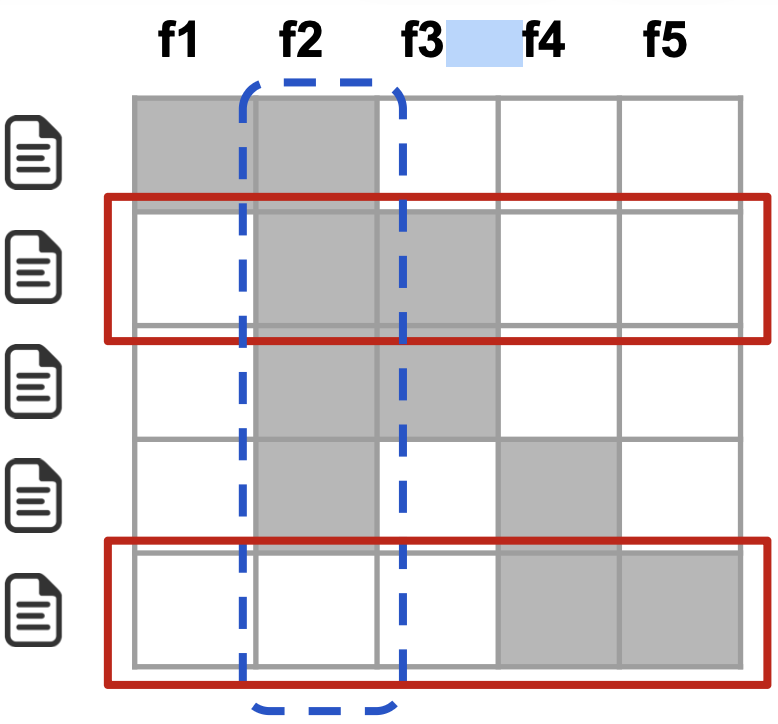
\includegraphics[width=0.2\linewidth]{images/SMP.png}
				}{}
				\caption{Explanation Matrix : SubModular Pick Algorithm}
				\label{fig:Explanation Matrix}
		\end{figure}
		
		
		\subsubsection{Advantages / Disadvantages}
		
		\begin{itemize}
		    \item Model-agnostic and flexible across data types.
		    \item Provides local, interpretable explanations.
		    \item Useful for debugging and decision transparency.
		    \item Helps explain individual outcomes (e.g., rejection cases).
		    \item Perturbations may generate unrealistic samples.
		    \item Sensitive to kernel width and surrogate model complexity.
		    \item Linear surrogate may fail for highly non-linear decision boundaries.
		    \item Interpretable representation may not capture all behaviors.
		\end{itemize}
		%------------------------------------------------------
		\subsection{Partial Dependency Plot}
		\begin{itemize}
			\item Visual tools to understand how features affect predictions, especially for complex, black-box models
			\item Shows the average effect of a feature on the model’s prediction, marginalizing over all other features.
	
			\item Pick a feature $X_j$
			\item Choose a grid of values for this feature
			\item For each such value:
				\subitem Replace the feature with that value in all instances.
				\subitem Predict using the model
				\subitem Average predictions across all instances
				\subitem Plot average predictions over the selected grid of values
			\item Model agnostic
			\item Example : As age increases, predicted risk increases
			\item Unrealistic data combinations
		\end{itemize}
		\begin{figure}[H]
			\centering
			\IfFileExists{images/PDP Plots.png}{
				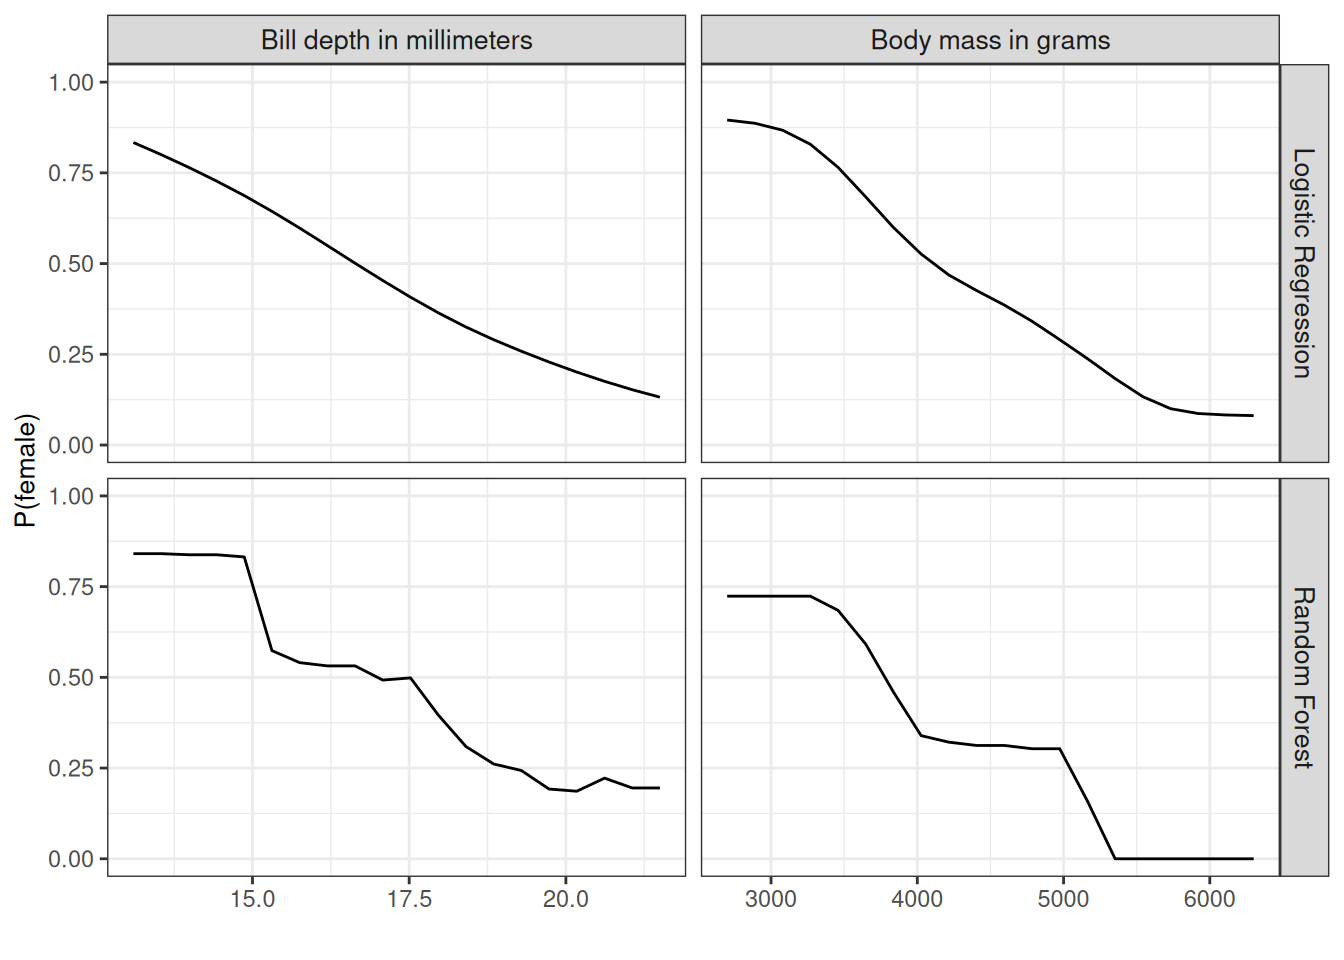
\includegraphics[width=0.6\linewidth]{images/PDP Plots.png}
			}{}
			\caption{Examples of PDP Plots with respect to two different models}
			\label{fig:Examples of PDP Plots}
		\end{figure}
		%------------------------------------------------------
		\subsection{ICE - Individual Conditional Expectation Plot}
		\begin{figure}[H]
				\centering
				\IfFileExists{images/svm_main.jpeg}{
					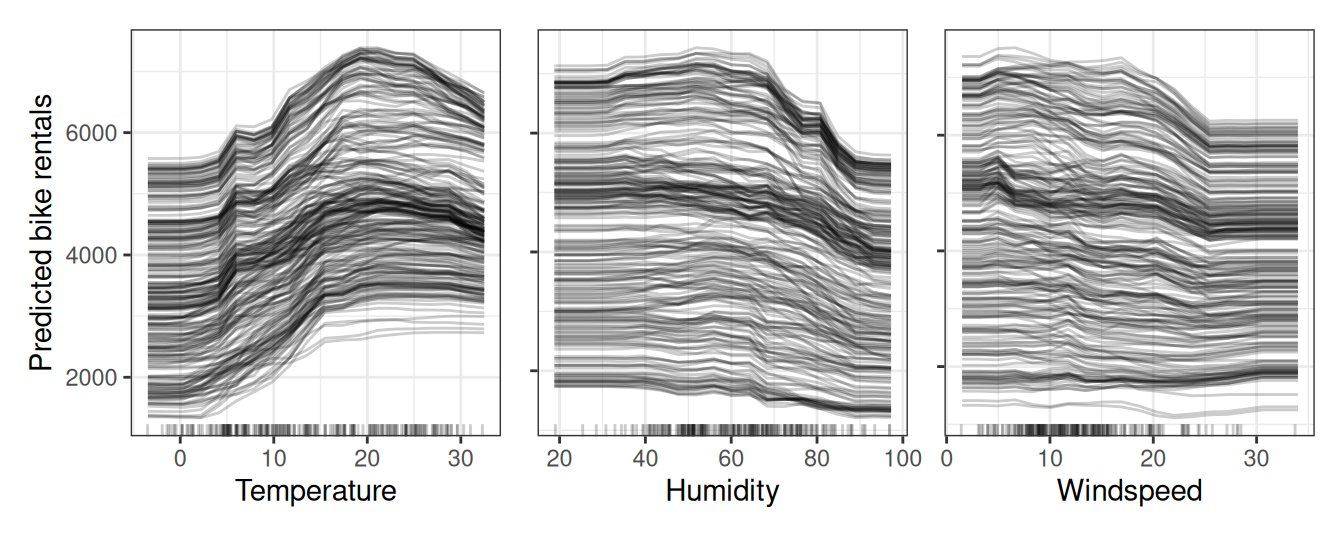
\includegraphics[width=0.6\linewidth]{images/ICE Plots.png}
				}{}
				\caption{Examples of ICE Plots}
				\label{fig:Examples of ICE Plots}
			\end{figure}
		\begin{itemize}
			\item Individual Conditional Expectation (ICE) plots display one line per instance that shows how the instance’s prediction changes when a feature changes
			\item Visualizes the dependence of the prediction on a feature for each instance separately, resulting in one line per instance of a dataset.
			\item The values for a line (and one instance) can be computed by keeping all other features the same, creating variants of this instance by replacing the feature’s value with values from a grid, and making predictions with the black box model for these newly created instances. The result is a set of points for an instance with the feature value from the grid and the respective predictions.
			
		\end{itemize}


	\section{Model Calibration}

	Calibration is the process of ensuring that the predicted probabilities from a model align well with the actual probabilities in the real world

	If a classification model outputs a probability of 0.80 for an event occurring, it should mean that on average the event occurs 80% of the time when the model predicts 0.8.  If this is not the case then the model is miscalibrated.

	\begin{itemize}
		\item For 100 customers, the prediction is 0.7 for churn
		\item So we expect out of this 100, about 70 customers should actually churn.
		\item If 80 got churn then it was underestimation
		\item If 50 got churn then it was over estimation
	\end{itemize}

	\subsection{Steps in Model Calibration}

	\begin{itemize}
		\item Train the model on the training set.
		\item Get predictions (probabilities) on the validation/calibration set.
		\item Fit the calibration method (Platt scaling, isotonic regression) using predicted probabilities as inputs and actual labels as targets.
		\item Apply the learned calibration function to the validation set (for checking) the test set (final evaluation) any future unseen data
	\end{itemize}

	\subsection{Brier Score Loss}

	Measures mean squared error between predicted probability and the actual label

	Overconfident wrong predictions → Higher Brier Score

	$$	\text{Brier Score = Reliability - (Resolution + Uncertainty)}
	$$
	$$	\text{Brier} = \frac{1}{N} \sum_{i=1}^{N} (p_i - y_i)^2
	$$
	$$	\text{Calibration Error / Reliability} =  \sum_{b=1}^{B} \frac{n_b}{N} (p_b - \bar{y}_b)^2
	$$
	$$	\text{Resolution/Discrimination} =  \sum_{b=1}^{B} \frac{n_b}{N} ( \bar{y}_b - \bar{y})^2
	$$
	$$	\text{Uncertainty} = \bar{y} ( 1- \bar{y})
	$$
	\begin{itemize}
		\item Resolution checks if the observed proportion differs from the average proportion.
		\item Reliability checks if average predicted probability matches the actual proportion in that bin.
	\end{itemize}

	\begin{itemize}
		\item Above diagonal → Under Confident
		\item Below diagonal → Over Confident
	\end{itemize}


	\subsection{Platt Scaling}
	\textbf{Making calibrated probabilities using Platt Scaling}

	Given the uncalibrated probabilities from my model and the true target labels, I can train a logistic regression on these probabilities to learn the coefficients A and B, and then use the learned sigmoid function

	$$	P_{\text{calibrated}} = \frac{1}{1+\exp{(Af+B)}}
	$$
	to transform the uncalibrated probabilities into calibrated probabilities.

	\subsection{Isotonic Regression}
	Isotonic regression is yet another method for getting calibrated probabilities.

	Isotonic regression is used when you believe:
	\begin{itemize}
		\item as x increases, y should not decrease.
		\item Higher dosage → higher (or no-worse) effect
		\item Higher hours studied → higher score
		\item Larger sample size → equal or better accuracy
		\item A risk score → non-decreasing probability
		\item In real data, noise may break monotonicity (y sometimes goes down when x goes up).
		\item Isotonic regression fixes that noise.
	\end{itemize}

	\subsubsection{Why We Need Isotonic Regression}

	\begin{itemize}
		\item Used when we know or assume the true relationship between variables should be \textbf{monotonic} (non-decreasing).
		\item Real data may violate monotonicity due to noise.
		\item Isotonic regression produces a \textbf{monotone, smoothed fit} that stays close to the original data.
	\end{itemize}

	\textbf{Typical use cases:}
	\begin{itemize}
		\item Machine learning probability calibration.
		\item Dose–response relationships in biology/medicine.
		\item Economics (price vs. demand).
		\item Any setting where monotonicity is known to hold.
	\end{itemize}

	\subsubsection{What Isotonic Regression Does}

	\begin{itemize}
		\item Given sorted data points
		$$ (x_1, y_1), (x_2, y_2), \ldots, (x_n, y_n), \quad x_1 \le x_2 \le \cdots \le x_n $$
		\item Find fitted values (Uncalibrated probabilities from the model )
		$$ \hat{y}_1, \hat{y}_2, \ldots, \hat{y}_n $$
		\item That satisfy the \textbf{monotonicity constraint}
		$$ \hat{y}_1 \le \hat{y}_2 \le \cdots \le \hat{y}_n $$
		\item And minimize squared error
		$$ \min_{\hat{y}} \sum_{i=1}^n (y_i - \hat{y}_i)^2 $$
	\end{itemize}

	\subsubsection{Block Averaging Idea}

	\begin{itemize}
		\item If a block \( B \) of consecutive points must share the same fitted value, the optimal value is
		$$ \hat{y}_B = \frac{1}{|B|} \sum_{i \in B} y_i $$
	\end{itemize}

	\begin{itemize}
		\item In weighted form (optional):
		$$ \hat{y}_B = \frac{\sum_{i \in B} w_i y_i}{\sum_{i \in B} w_i} $$
	\end{itemize}


	\subsubsection{Pool-Adjacent-Violators (PAV) Algorithm}

	\begin{itemize}
		\item \textbf{Step 1 — Initialization}
		\item Treat each point as its own block.
		\item Block $ B_i = \{i\} $, value $ v_i = y_i $, weight $ w_i = 1 $
		\item Here, we have uncalibrated probabilities and actual labels, values are the actual labels.
	\end{itemize}

	\begin{itemize}
		\item \textbf{Step 2 — Scan left to right}
		\item For adjacent blocks $ B_i, B_{i+1} $
		\item If $ v_i \le v_{i+1} $, continue.
		\item If $ v_i > v_{i+1} $, a \textbf{violation} occurs → merge blocks.
	\end{itemize}

	\begin{itemize}
		\item \textbf{Step 3 — Merge Violating Blocks}
		\item New block weight:
		$$ w = w_i + w_{i+1} $$
		\item New block value:
		$$ v = \frac{w_i v_i + w_{i+1} v_{i+1}}{w_i + w_{i+1}} $$
	\end{itemize}

	\begin{itemize}
		\item \textbf{Step 4 — Backward Check}
		\item After merging, check previous block.
		\item If previous block value > new block value → merge again.
		\item Repeat until monotonicity is restored.
	\end{itemize}

	\begin{itemize}
		\item \textbf{Step 5 — Form Final Fitted Values}
		\item Each block produces constant fitted values:
		$$ \hat{y}_i = \hat{y}_{i+1} = \cdots = \hat{y}_j = v_B \quad \text{for block } B = \{i,\ldots,j\} $$
	\end{itemize}


	\subsubsection{Interpretation}

	\begin{itemize}
		\item Output is a \textbf{piecewise-constant, non-decreasing function}.
		\item It removes random decreases in data while staying close to observations.
		\item The final fit is the \textbf{closest possible monotone sequence} to the original data in squared-error sense.
	\end{itemize}

	\subsubsection{Numeric Example : Isotonic Regression}

	\begin{center}
		\begin{tabular}{lccc}
			\toprule
			Point & Predicted & Label & Calibrated (PAV) \\
			\midrule
			A & 0.1 & 0 & 0 \\
			B & 0.2 & 1 & 0.6667 \\
			C & 0.3 & 1 & 0.6667 \\
			D & 0.4 & 0 & 0.6667 \\
			E & 0.5 & 1 & 1 \\
			\bottomrule
		\end{tabular}
	\end{center}

	\begin{itemize}
		\item Sort the data by predicted probability. We order the points based on their uncalibrated scores so that the probability axis is monotone, even if the labels are not.
		\item Start with each point as a block. Each block has a temporary “fitted value” equal to its label.
		\item Scan left → right and find monotonicity violations. A violation occurs when a block on the left has a higher value than the next block on the right.
		\item Merge violating blocks. When two blocks violate monotonicity, we replace them with a single block whose value is the weighted average of the labels in that block. This average becomes the new calibrated probability for all points in that merged block.
		\item Backward check. After merging, we check whether the new block violates monotonicity with the block before it. If so, we merge again. This continues until all block values are non-decreasing.
		\item Final output- Once all violations are resolved, every block has a constant fitted value. These fitted values are the calibrated probabilities,forming a piecewise-constant, non-decreasing function that is optimally close to the true labels under squared error.
	\end{itemize}


	\subsection{Platt or Isotonic Regression ?}

	\textbf{Platt scaling} and \textbf{isotonic regression} are techniques to calibrate machine learning model probabilities. Platt scaling fits a sigmoid function (effective for SVMs/small data), while isotonic regression fits a non-parametric, monotonic function (better for large data/complex distortions, but prone to overfitting).
	Key Differences and Selection Criteria
	\begin{itemize}
		\item Platt Scaling (Logistic Calibration):
		\item Best for: Small calibration datasets (< 1000 samples).
		\item Method: Fits a logistic regression model (sigmoid curve) to the predicted scores.
		\item Pros: Less prone to overfitting, works well when the distortion is sigmoid-shaped (e.g., SVMs, boosted trees).
		\item Cons: Limited to monotonic, sigmoid-shaped corrections.
		\item Isotonic Regression:
		\item Best for: Large calibration datasets (> 1000 samples).
		\item Method: Fits a non-decreasing, free-form, piecewise-constant function (non-parametric).
		\item Pros: More powerful, can correct any monotonic distortion.
		\item Cons: Prone to overfitting on small data.
	\end{itemize}

	When to Use Which?
	\begin{itemize}
		\item Use Platt Scaling if your dataset is small or you have limited, high-confidence prior knowledge that the error is sigmoidal.
		\item Use Isotonic Regression if you have a large dataset, which helps prevent it from fitting noise (overfitting).
	\end{itemize}



	\section{Feature Selection}
	\subsection{Filter Methods}
	\subsubsection{Mutual Information}

	\begin{itemize}
		\item Mutual information is a filter method
		\item It selected features only on their relationship with the target, not on any trained model.
		\item A feature is good if it tells you a lot about the target.
		\item How much knowing X reduces uncertainty about Y.
		\item Feature and target are independent → MI=0
		\item Strong dependence → MI is large.
		\[
		I(X,Y) = \sum_{x \in X}^{} \sum_{y \in Y}^{} p(x,y) \log \frac{p(x,y)}{p(x)p(y)}
		\]
	
		\item if features are independent then MI will be 0.
		
		\[
		H(Y) = - \sum_{y}^{} p(y) \log p(y)
		\]

		\[
		H(Y|X) = - \sum_{x,y}^{} p(x,y) \log p(y|x)
		\]
		
		\[
		I(X;Y) = H(Y) - H(Y|X)
		\]

		\item So, MI = Reduction in uncertainty about Y when X is known.
	\end{itemize}
	
	\subsubsection{ANOVA For Feature Selection}
	\begin{itemize}
		\item Used mainly for classification tasks with a categorical target.
		\item Does the mean of the feature vary between classes.
		\item Anova computes the ratio of variance between classes to variance within classes.
	\end{itemize}

	$$	F = \frac{\text{Variance between classes}}{\text{Variance within classes}}
	$$
	\begin{itemize}
		\item We have a feature $X_j$
		\item Classes $C_1, C_2, \ldots, C_k$
		\item Number of samples $n_i$ in class $i$
		\item $\bar{x}_i$ be the mean of feature in class i
		\item $\bar{x}$ be the overall mean of the feature
		\item Compute the between and within class variance and then the f statistic using the following equations.
	\end{itemize}

	\[
	SSB_j = \sum_{c=1}^{k} \sum_{i=1}^{n_c} (\bar{x}_{c j} - \bar{x}_j)^2 = \sum_{c=1}^{k} n_c \, (\bar{x}_{c j} - \bar{x}_j)^2
	\]
	
	
	$$SSW_j = \sum_{i=1}^{k} \sum_{x \in C_i}^{} (x-\bar{x}_i)^2
	$$
	Between class sum of squares measures how much the class means deviate from overall mean.
	
	Within class sum of squares measure the variability inside each class.

	\[
	F_j = \frac{SSB_j/(k-1)}{SSW_j/(N-k)} \sim F_{\,k-1,\;N-k}
	\]
	
	\begin{itemize}
		\item High $F_j$ → Feature strongly separates classes
		\item Low $F_j$ → Feature weakly separates classes
		\item It only captures differences in mean ( ignores variance structure, interactions)
	\end{itemize}
	
	\[
	\text{Decomposition} ;  \sum_{j=1}^{k} \sum_{i=1}^{n_j} (x_{ij} - \bar{x})^2
	=
	\sum_{j=1}^{k} n_j (\bar{x}_j - \bar{x})^2
	+
	\sum_{j=1}^{k} \sum_{i=1}^{n_j} (x_{ij} - \bar{x}_j)^2
	\]

	\subsubsection{Variation Inflation Factor - VIF}

	\begin{itemize}
		\item High VIF → Feature is highly correlated with others → May consider removing it.
	\end{itemize}

	$$	VIF_j = \frac{1}{1-R_j^2}
	$$
	\begin{itemize}
		\item If $X_j$ feature is highly predictable from other features implies High VIF.
		\item $1 < VIF < 5$ implies Moderate correlation
		\item $VIF>5$ implies Higher correlation, consider removing
	\end{itemize}

	\subsubsection{Weight of Evidence}

	How strongly a feature value ( or bin) separates good vs bad customers.

	$$	\text{Weight of Evidence} = \log \left(\frac{\text{\% of Good in the bin}} {\text{\% of Bad in the bin}} \right)
	$$
	\begin{itemize}
		\item Is this bin more associated with good or bad outcome?
		\item For continuous features we can use equal width bins or optimal binning.
		\item After this, we can compute the Information Value ;
	\end{itemize}

	$$	IV = \sum_{i} (\text{\% of Good} - \text{\% of Bad}) * WoE
	$$
	\begin{itemize}
		\item if $IV>0.3$ then the predictor is strong
		\item if $IV <0.1$ its a weak predictor
	\end{itemize}

	\subsubsection{Chi-Square Test of Independence}

	\begin{itemize}
		\item A feature is useful , when its distribution is different across classes.
		\item A feature is informative when it is dependent of target.
		\item Null Hypothesis : X \& Y are independent
		\item We create the contingency table.
		\item We compute the expected counts
		\item Compute the chi-square statistic
	\end{itemize}
	\[
	E_{ij} = \frac{(\text{Row i Total}) * (\text{Column j Total})}{N}
	\]
	
	\[
	\chi^2 = \sum_{i,j} \frac{(O_{ij} - E_{ij})^2}{E_{ij}}
	\]
	
	If we have r categories in the feature and c classes in the target column, then the degrees of freedom will be $(r-1) (c-1)$
	\begin{center}
		\begin{tabular}{|c|c|c|c|}
			\hline
			 & Purchase = Yes & Purchase = No & Row Total \\
			\hline
			Coupon = Yes & 40 & 10 & 50 \\
			\hline
			Coupon = No & 20 & 30 & 50 \\
			\hline
			Column Total & 60 & 40 & 100 \\
			\hline
			\end{tabular}
			
			\vspace{1em}
			
			\begin{tabular}{|c|c|c|}
			\hline
			 & Purchase = Yes & Purchase = No \\
			\hline
			Coupon = Yes & 30 ($=50\times60/100$) & 20 ($=50\times40/100$) \\
			\hline
			Coupon = No & 30 ($=50\times60/100$) & 20 ($=50\times40/100$) \\
			\hline
			\end{tabular}
	\end{center}
	

	\subsection{Wrapper Methods in Feature Selection}

	\begin{itemize}
		\item Iterative procedures
		\item One independent variable at a time is added or deleted based on the p-value.
	\end{itemize}

	\subsubsection{Forward Selection}
	
	Forward Selection is a greedy feature selection method where features are added sequentially based on performance improvement.
	
	\begin{itemize}
	    \item Start by selecting the single best feature (the one that gives the highest model performance).
	    \item At each subsequent step:
	    \begin{itemize}
	        \item Consider adding each remaining feature to the current selected set.
	        \item Train the model with each possible addition.
	        \item Evaluate performance using validation or cross-validation.
	        \item Select the feature that results in the highest performance improvement.
	    \end{itemize}
	    \item Add the chosen feature to the feature set.
	    \item Repeat this process iteratively.
	    \item Stop when no further significant improvement is observed or a predefined stopping criterion is met.
	\end{itemize}

	\subsubsection{Backward Elimination}
	
	Backward Elimination is a greedy feature selection method where features are removed sequentially based on their impact on model performance.
	
	\begin{itemize}
	    \item Start with the full set of features.
	    \item At each step:
	    \begin{itemize}
	        \item Consider removing each feature one at a time.
	        \item Train the model on the remaining feature set after each removal.
	        \item Evaluate performance using validation or cross-validation.
	        \item Identify the feature whose removal leads to the best performance (or least decrease in performance).
	    \end{itemize}
	    \item Remove the selected feature permanently.
	    \item Repeat this process iteratively.
	    \item Stop when removing any further feature significantly degrades performance or a stopping criterion is met.
	\end{itemize}

	\subsubsection{Stepwise Selection}
	
	Stepwise Selection is a hybrid feature selection method that combines forward selection and backward elimination. At each step, it allows both addition and removal of features based on model performance.
	
	\begin{itemize}
	    \item Start with an empty set of features (or optionally a predefined set).
	    \item Perform forward selection:
	    \begin{itemize}
	        \item Add the feature that gives the highest improvement in performance.
	    \end{itemize}
	    \item After adding a feature, perform backward elimination:
	    \begin{itemize}
	        \item Check if any feature in the current set can be removed without degrading performance.
	        \item Remove the feature whose removal improves or least affects performance.
	    \end{itemize}
	    \item Repeat the process:
	    \begin{itemize}
	        \item Alternate between adding and removing features.
	    \end{itemize}
	    \item Stop when:
	    \begin{itemize}
	        \item No feature can be added to improve performance, and
	        \item No feature can be removed without worsening performance.
	    \end{itemize}
	\end{itemize}

	\subsubsection{Recursive Feature Elimination}

	\begin{itemize}
		\item In backward elimination the removal is based on; Which feature can I remove with the least drop in model performance?
		\item In RFE the removal is based on which feature is least important according to the model itself ?
		\item so we train model once, get the feature importance scores, coefficients , then remove the weakest, retrain and repeat.
		\item Backward Elimination: If I remove you, what happens to performance?
		\item RFE : How important does the model think you are?
	\end{itemize}
	
	
	\subsubsection{Rfecv Algorithm}
	
	Recursive Feature Elimination with Cross Validation selects features iteratively.
	\begin{itemize}
		\item Input: Dataset $X, y$, estimator (model), number of folds $k$

		\item Initialize with all features

		\item Repeat until stopping criterion:
		\begin{itemize}
			\item Perform $k$-fold cross-validation:
			\begin{itemize}
				\item Train the model on training folds
				\item Evaluate performance on validation fold
			\end{itemize}

			\item Compute average validation score across folds

			\item Rank features based on model importance (e.g., coefficients or feature importance)

			\item Remove the least important feature(s)
		\end{itemize}

		\item Track cross-validation score for each number of features

		\item Select the number of features that gives the best cross-validation performance

		\item Output: Optimal subset of features
	\end{itemize}

	\subsection{Embedded Methods in Feature Selection}

	\subsubsection{Lasso - L1 Regularisation}

	\begin{itemize}
		\item Feature selection happens automatically during training.
		\item Add a penalty that pushes coefficients to exactly zero.
		\item L1 penalty has a diamond shaped constraint.
		\item Optimal solution often hits the corners.
	\end{itemize}
	
	\[
	\lambda \sum_j |\beta_j|
	\]

	\begin{itemize}
		\item As lambda increases small coefficients shrink to 0 first.
		\item Non-zero coefficients = selected features.
	\end{itemize}
	
	\subsubsection{Tree Methods}
	Tree-based methods perform feature selection during model training by choosing splits based on feature importance.
	
	\begin{itemize}
	    \item At each split, the feature that maximizes a criterion (e.g., Gini impurity, information gain) is selected.
	    \item Irrelevant features are not used in splits and are implicitly ignored.
	    \item Common models: Decision Trees, Random Forests, Gradient Boosted Trees (XGBoost, LightGBM, CatBoost).
	    \item Feature importance is computed via total impurity reduction or gain.
	    \item No separate feature selection step is required.
	\end{itemize}

	\subsection{Tree-based Feature Importance}
	\begin{itemize}
		\item impurity based feature importance
		\item A feature is important if it is used often to split nodes and the split reduce uncertainty a lot.
		\item Importance = How much total impurity this feature removes across the whole forest.
		\item We have impurity measures like Gini, Entropy, Variance(MSE). We can compute the impurity difference between parent and child node. The impurity decrease is the value which is credited to the feature used in that split.
		\item For a feature we can compute the the entire impurity reductions over the tree. And we can normalize it ( based on other feature’s importance)
		\item If we have T trees then we can again take the sum and normalize it.
	\end{itemize}

	$$	\text{Importance(f)} = \sum_{s \in S_f} \Delta I_s
	$$
	Here $\Delta_s$ is the impurity decrease at split s

	Following equation gives the feature importance in one tree;

	$$	\text{Normalized Importance(f)} = \frac{\text{Importance(f)}}{\sum_j \text{Importance(j)}}
	$$
	Now we have T trees ;

	$$	\text{Importance(f)} = \frac{1}{T} \sum_{t=1}^{T} \text{Importance(f)}
	$$
	And after this we can normalize again to get the value between 0 and 1.

	\begin{itemize}
		\item This approach is biased towards continuous variables.
		\item High-cardinality categorical features.
		\item If A and B are correlated ; Tree may pick only one. Other gets low importance even if its meaningful.
	\end{itemize}

	\subsection{Permutation Feature Importance}

	\begin{itemize}
		\item Model agnostic, performance based
		\item If feature is important, breaking its relationship with the target should hurt performance.
		\item We do this by ;
			\subitem Randomly shuffling one feature column in the validation set.
			\subitem Keeping everything else the same
			\subitem Measuring how much the model performance drops
			\subitem Importance = Performance drop
		\item Algorithm
			\subitem 1. Train model on training set
			\subitem 2. Evaluate on validation set - get $M_{\text{base}}$
			\subitem For each feature j:
				\subsubitem Copy dataset
				\subsubitem Randomly permute column j in the validation set
				\subsubitem Predict with trained model
			\subitem Compute new performance $M_j$
			\subitem Importance = Difference from baseline
		\item Rank features by importance → Normalize
		\item We can use repeated permutations also and take the average for computing $M_j$
		\item Issues : If two features are correlated , shuffling one might not hurt much, because model can still use the other feature.
	\end{itemize}

	\subsection{Drop-column}

	\begin{itemize}
	\item Remove feature $X_j$ completely from dataset
	\item Train a new model $f_{-j}$ on remaining features
	\item Compute importance via performance drop:
	\item Measures: \textbf{true predictive contribution} of $X_j$
	\item Model is different after dropping $\Rightarrow$ allows re-optimization
	\item \textbf{Key Properties}
	\begin{itemize}
	    \item Captures whether feature is \textbf{necessary} for prediction
	    \item Accounts for \textbf{feature redundancy} (via retraining)
	    \item If correlated features exist $\Rightarrow$ importance may be low
	\end{itemize}
	
	\item \textbf{Pros and Cons}
	\begin{itemize}
	    \item Suitable for feature selection
	    \item Model Agnostic
	    \item Computationally expensive (retrain for each feature)
	    \item Not explaining the original trained model
	\end{itemize}
	\end{itemize}


	\section{Information Theory Concepts}

	\subsection{Entropy}
	In information theory, entropy is a measure of uncertainty or randomness in a set of data. The more unpredictable or random the data, the higher its entropy.
	\begin{align*}
		\large H(X) = -\sum_{i=1}^{n} P(x_i) \log_2(P(x_i))
	\end{align*}
	\begin{itemize}
		\item Probability and surprice is inveserly related.
		\item when the probability is 1, the surprice needs to be zero, for this reason we can not say that surprice is 1/p. So surprice is defined as $log(1/p)$.
		\item Entropy can be defined as expected value of surprice.
		\item In summary, the entropy is a measure of the average amount of surprise or information content associated with a set of outcomes. If all outcomes are equally likely, the entropy is maximized, indicating maximum uncertainty. If some outcomes are more likely than others, the entropy is reduced, reflecting a lower level of uncertainty.
	\end{itemize}


	\subsection{Cross Entropy Loss}

	Cross -entropy loss or log loss measures the performance of a classification model whose output is a probability value between 0 and 1. Cross entropy loss increases as the predicted probability diverges from the actual label.
	In binary classification, where the number of classes is two, cross entropy can be calculated as follows ;

	\begin{align*}
		\large-(y*log(p) + (1-y) * log(1-p))\LARGE
	\end{align*}

	In multi-classification scenario, we calculate separate loss for each class label per observation and sum the result.

	\begin{align*}
		\large    -\sum_{c=1}^{M} y*log(p) \LARGE
	\end{align*}

	\subsection{Joint Entropy}

	Joint entropy is a measure of uncertainty associated with a joint probability distribution of two or more random variables. It is an extension of the concept of entropy, which is used to quantify the uncertainty or information content of a single random variable. Joint entropy takes into account the uncertainty of multiple variables occurring together.

	For two random variables, X and Y, with a joint probability distribution $P(X,Y)$,
	the joine entropy, $H(X,Y)$ is given by:

	\begin{align*}
		\large H(X, Y) = -\sum_{i=1}^{m} \sum_{j=1}^{n} P(x_i, y_j) \log_2(P(x_i, y_j))
	\end{align*}

	Joint entropy provides a measure of the average amount of uncertainty or information content associated with the joint occurrences of the two random variables. If X and Y are independent, meaning the occurrence of one does not provide information about the other, then the joint entropy is the sum of the individual entropies:
	$ H(X,Y) = H(X)+H(Y)$

	However, if X and Y are dependent, the joint entropy will be less than the sum of the individual entropies, reflecting the reduced uncertainty when the variables are considered together.

	\subsection{Mutual Information}
	Mutual information is a measure of the amount of information that knowing the value of one random variable provides about another random variable. It quantifies the reduction in uncertainty about one variable when the value of the other variable is known. Mutual information is widely used in information theory, statistics, and machine learning.

	for two discreet random variable X,Y, with probability distribution $P(X,Y)$,the mutual information $I(X;Y)$ is given by:

	\begin{align*}
		\large I(X; Y) = \sum_{i=1}^{m} \sum_{j=1}^{n} P(x_i, y_j) \log_2\left(\frac{P(x_i, y_j)}{P(x_i)P(y_j)}\right)
	\end{align*}

	Mutual information measures the reduction in uncertainty about one variable (x) given knowledge of the other variable(y). If x and y are independent then $I(x,y) = 0$, indicating that knowing the value of y provides no information about x, and vice versa. On the other hand if X and Y are dependent, $I(x,y)$ is positive, indicating that knowledge of one variable can reduce uncertainty about the other.

	It is important to note that mutual information is symmetric. It can be used to quantify the relationship between any two random variables.

	\subsection{KL Kullback-Leibler Divergence}
	\label{kldivergence}
	This is also known as relative entropy. Measure of how one probability distribution diverges from a second, expected probability distribution. i its commonly used in information theory to quantify the difference between two probability distributions.

	\begin{align*}
		\large D_{\text{KL}}(P \| Q) = \sum_{i} P(i) \log\left(\frac{P(i)}{Q(i)}\right)
	\end{align*}

	\begin{itemize}
		\item KL divergence is not symmetric
		\item if p and q are same, then kl divergence is zero
		\item always non-negative
		\item unbounded
	\end{itemize}

	The interpretation of KL divergence is that it measures the extra average number of bits needed to represent events from P using a code optimized for Q, compared to using a code optimized for P. In other words, it quantifies the inefficiency in using the wrong probability distribution Q to represent the true distribution P.



	\subsection{Population Stability Index}

	PSI measures how much a variable’s distribution has changed between

	\begin{itemize}
		\item a reference dataset ( training  or baseline )
		\item a current dataset ( new or live )
	\end{itemize}

	Has the population changed compared to what the model was trained on ?

	\begin{itemize}
		\item Suppose we have a feature, the first step is to divide it into bins ( equal width or equal frequency)
		\item For each bin compute the proportions from reference data and the current data.
	\end{itemize}

	$$	\Large PSI = \sum_{Bin} (p_i - q_i)  \log\left(\frac{p_i}{q_i}\right)
	$$
	\begin{itemize}
		\item Here, p is the reference ( training or baseline)
		\item Sum over all bins, then we get the PSI
		\item If value is $<$ 0.1 then No significant change
		\item If value is 0.1 to 0.25 then moderate shift
		\item If value is $>$ 0.25 then major population drift
	\end{itemize}

	\subsection{Identities and Inequalities}
	
	\textbf{Ranges and Bounds}
	
	\begin{itemize}
	\item $0 \le H(X) \le \log |\mathcal{X}|$ ( Uniform Distribution)
	\item $0 \le H(Y|X) \le H(Y)$
	\item $\max{H(X), H(Y)} \le H(X,Y) \le H(X) + H(Y)$
	\item $0 \le I(X;Y) \le \min{H(X), H(Y)}$
	\item $D_{KL}(p | q) \ge 0$
	\item $H(p,q) \ge H(p)$
	\end{itemize}
	
	\vspace{0.5em}
	
	\textbf{Core Identities}
	
	\begin{equation*}
	H(X,Y) = H(X) + H(Y|X)
	\end{equation*}
	
	\begin{equation*}
	H(X,Y) = H(Y) + H(X|Y)
	\end{equation*}
	
	\begin{equation*}
	H(X_1, \dots, X_n) = \sum_{i=1}^n H(X_i \mid X_1, \dots, X_{i-1})
	\end{equation*}
	
	\begin{equation*}
	I(X;Y) = H(X) - H(X|Y)
	\end{equation*}
	
	\begin{equation*}
	I(X;Y) = H(Y) - H(Y|X)
	\end{equation*}
	
	\begin{equation*}
	I(X;Y) = H(X) + H(Y) - H(X,Y)
	\end{equation*}
	
	\begin{equation*}
	H(p,q) = H(p) + D_{KL}(p | q)
	\end{equation*}
	
	\vspace{0.5em}
	
	\textbf{Important Inequalities}
	
	\begin{itemize}
	\item $H(Y|X) \ge 0$
	\item $H(Y|X) \le H(Y)$
	\item $H(X,Y) \le H(X) + H(Y)$
	\item $H(X,Y) = H(X) + H(Y) ;; \text{iff } X \perp Y$
	\item $D_{KL}(p | q) \ge 0$
	\item $I(X;Y) \ge 0$
	\item $I(X;Y) \le H(X)$, \quad $I(X;Y) \le H(Y)$
	\end{itemize}
	

	\section{Principal Component Analysis (PCA)}

	\subsection{Goal and Intuition}

	Principal Component Analysis (PCA) is a technique for \textbf{dimensionality reduction}. It transforms the original features into a new set of orthogonal variables called \textbf{principal components}.

	These components are constructed so that:

	\begin{itemize}
		\item They are \textbf{uncorrelated}.
		\item They capture the \textbf{maximum possible variance} in the data.
	\end{itemize}

	The components are ordered by importance:

	\begin{itemize}
		\item The \textbf{first principal component} captures the largest variance.
		\item The \textbf{second principal component} captures the next largest variance while being orthogonal to the first.
		\item This continues for all remaining components.
	\end{itemize}

	Thus PCA finds new axes that best describe the spread of the data.
	Before applying PCA, the dataset must be centered.

	\[
	x_i \leftarrow x_i - \mu
	\]

	where $\mu$ is the mean of each feature.

	Centering ensures that PCA finds directions of maximum variance relative to the origin.

	PCA can be understood as projecting data onto a new direction.

	Project a vector $x$ onto a \textbf{unit vector} $u$:

	\[
	\text{proj}_u(x) = (u^T x)u
	\]

	\begin{itemize}
		\item $u$ is a unit vector defining a direction.
		\item $u^T x$ represents the scalar component of $x$ along that direction.
	\end{itemize}

	PCA finds the directions onto which projections of the data have the largest variance.

	\subsection{Steps of PCA}

	\begin{itemize}

		\item Standardize or center the data.

		\item Compute the \textbf{covariance matrix}

		\begin{itemize}
			\item Diagonal elements represent feature variances.
			\item Off-diagonal elements represent covariances between features.
		\end{itemize}

		\item Compute the \textbf{eigenvalues} and \textbf{eigenvectors} of the covariance matrix.

		\item Sort eigenvectors according to decreasing eigenvalues.

		\item Select the top $k$ eigenvectors.

		\item Project the data onto these directions.

	\end{itemize}

	\subsection{Eigenvectors and Eigenvalues}

	\begin{itemize}

		\item Eigenvectors define the directions of the principal components.

		\item Eigenvalues represent the amount of variance captured in those directions.

		\item Larger eigenvalues correspond to directions with greater variability in the dataset.

		\item Eigenvectors corresponding to distinct eigenvalues are linearly independent.

	\end{itemize}

	\subsection{Explained Variance}

	Each eigenvalue indicates how much variance is explained by its corresponding principal component.

	If the eigenvalues are

	\[
	\lambda_1, \lambda_2, ..., \lambda_p
	\]

	then the proportion of variance explained by component $k$ is

	\[
	\frac{\lambda_k}{\sum_{i=1}^{p}\lambda_i}
	\]

	This helps determine how many components should be retained.


	\subsection{Covariance Matrix and Positive Semi-Definite Property}

	The covariance matrix has two important properties:

	\begin{itemize}
		\item It is \textbf{symmetric}
		\item It is \textbf{positive semi-definite (PSD)}
	\end{itemize}

	A matrix $A$ is positive semi-definite if

	\[
	x^T A x \ge 0
	\]

	for every vector $x$.

	\subsection{Why Covariance Matrices are PSD}

	For a covariance matrix $\Sigma$,

	\[
	x^T \Sigma x = Var(x^T X)
	\]

	Variance is always non-negative, therefore

	\[
	x^T \Sigma x \ge 0
	\]

	This proves that covariance matrices are positive semi-definite.

	The PSD property guarantees that:

	\begin{itemize}
		\item All eigenvalues of the covariance matrix are \textbf{non-negative}.
		\item Variance captured by principal components cannot be negative.
		\item Eigenvectors form valid orthogonal directions for projection.
	\end{itemize}

	Thus PCA provides a meaningful decomposition of variance in the data.

	\subsection{Connection to Singular Value Decomposition (SVD)}

	PCA can also be computed using Singular Value Decomposition.

	\[
	X = U \Sigma V^T
	\]

	In this formulation:

	\begin{itemize}
		\item Columns of $V$ correspond to the principal directions.
		\item Singular values relate to the amount of variance explained.
	\end{itemize}

	Many machine learning libraries compute PCA using SVD because it is numerically more stable.


	\section{Recommendation Systems}

	\subsection{Goal of Recommendation Systems}

	A recommendation system tries to solve the following problem:

	\textbf{Given users, items, and interaction data, predict how much a user will like an item they have not interacted with yet.}


	Examples of interaction data:

	\begin{itemize}
		\item Ratings (1–5 stars)
		\item Clicks / views
		\item Purchases
		\item Likes / skips
		\item Watch time
	\end{itemize}

	These interactions are used to estimate user preferences and recommend relevant items.

	\subsection{Main Types of Recommendation Systems}

	\begin{itemize}

		\item \textbf{Content-Based Filtering}

		Recommend items that are \textbf{similar to the items a user liked in the past}.

		\item \textbf{Collaborative Filtering}

		Recommend items based on the behavior of \textbf{similar users or similar items}.

		\item \textbf{Matrix Factorization}

		A model-based collaborative filtering method that learns \textbf{latent representations of users and items}.

	\end{itemize}

	\subsection{Content-Based Filtering}
	Content-based filtering recommends items to a user based on the similarity between item features and the user's past preferences. Let $R \in \mathbb{R}^{m \times n}$ denote the user--item interaction matrix, and let $x_i \in \mathbb{R}^{d}$ represent the feature vector of item $i$ (e.g., genre, keywords, embeddings).

	\vspace{0.3em}

	A user profile vector is constructed from the items the user has interacted with. For user $u$, a common formulation is:
	\[
	p_u = \frac{\sum_{i \in I_u} r_{u,i}\, x_i}{\sum_{i \in I_u} r_{u,i}}
	\]
	where $I_u$ is the set of items rated (or interacted with) by user $u$.

	\vspace{0.3em}

	To estimate the preference of user $u$ for a new item $j$, compute the similarity between the user profile and the item feature vector.

	Cosine similarity:
	\[
	\hat{r}_{u,j} = \text{sim}(p_u, x_j) =
	\frac{p_u^\top x_j}{\|p_u\| \, \|x_j\|}
	\]

	\vspace{0.3em}

	Alternatively, a linear scoring function can be used:
	\[
	\hat{r}_{u,j} = p_u^\top x_j
	\]

	\vspace{0.3em}

	Thus, items whose features are most similar to the user's learned preference vector are recommended.

	\vspace{0.3em}

	This approach relies entirely on item features and does not require other users' data. It is effective when item metadata is rich and informative.

	\vspace{0.3em}

	Limitations include inability to capture collaborative signals, dependence on feature quality, and tendency to over-specialize (recommending items too similar to those already seen).


	\subsection{Collaborative Filtering}
	Users who behaved similarly in the past will have similar preferences in the future
	We start with a \textbf{user–item interaction matrix}:

	\[
	R =
	\begin{bmatrix}
		r_{1,1} & r_{1,2} & \dots \\
		r_{2,1} & r_{2,2} & \dots \\
		\vdots
	\end{bmatrix}
	\]

	This matrix is typically \textbf{sparse} since most users interact with only a small fraction of items.

	Collaborative filtering methods include:

	\begin{itemize}
		\item User-Based Collaborative Filtering
		\item Item-Based Collaborative Filtering
	\end{itemize}

	\subsubsection{User-Based Collaborative Filtering}
	User-based collaborative filtering predicts a user's preference based on the preferences of similar users. Let $R \in \mathbb{R}^{m \times n}$ denote the user--item rating matrix, where $r_{u,i}$ represents the rating given by user $u$ to item $i$.

	\vspace{0.3em}

	For two users $u$ and $v$, similarity is computed over the set of commonly rated items $I_{uv}$.

	Cosine similarity:
	\[
	\text{sim}(u,v) =
	\frac{\sum_{i \in I_{uv}} r_{u,i}\, r_{v,i}}
	{\sqrt{\sum_{i \in I_{uv}} r_{u,i}^2}\;
		\sqrt{\sum_{i \in I_{uv}} r_{v,i}^2}}
	\]

	Pearson correlation:
	\[
	\text{sim}(u,v) =
	\frac{\sum_{i \in I_{uv}} (r_{u,i} - \bar{r}_u)(r_{v,i} - \bar{r}_v)}
	{\sqrt{\sum_{i \in I_{uv}} (r_{u,i} - \bar{r}_u)^2}\;
		\sqrt{\sum_{i \in I_{uv}} (r_{v,i} - \bar{r}_v)^2}}
	\]
	where $\bar{r}_u$ is the mean rating of user $u$.


	For a target user $u$, define the neighborhood:
	\[
	N_k(u) = \text{Top-}k \text{ users with highest similarity to } u
	\]

	Prediction of rating for item $i$:

	Basic weighted average:
	\[
	\hat{r}_{u,i} =
	\frac{\sum_{v \in N_k(u)} \text{sim}(u,v)\, r_{v,i}}
	{\sum_{v \in N_k(u)} |\text{sim}(u,v)|}
	\]

	Mean-centered prediction:
	\[
	\hat{r}_{u,i} =
	\bar{r}_u +
	\frac{\sum_{v \in N_k(u)} \text{sim}(u,v)\, (r_{v,i} - \bar{r}_v)}
	{\sum_{v \in N_k(u)} |\text{sim}(u,v)|}
	\]


	The similarity acts as a weight, so more similar users contribute more to the prediction. Mean-centering adjusts for user-specific rating biases.


	Limitations include sparsity of the rating matrix, cold-start issues for new users or items, and computational cost of similarity calculations.

	\subsubsection{Item-Based Collaborative Filtering}
	Item-based collaborative filtering predicts a user's preference for an item based on their ratings of similar items. Let $R \in \mathbb{R}^{m \times n}$ denote the user--item rating matrix, where $r_{u,i}$ represents the rating given by user $u$ to item $i$.

	\vspace{0.3em}

	For two items $i$ and $j$, similarity is computed over the set of users who have rated both items, denoted by $U_{ij}$.

	Cosine similarity:
	\[
	\text{sim}(i,j) =
	\frac{\sum_{u \in U_{ij}} r_{u,i}\, r_{u,j}}
	{\sqrt{\sum_{u \in U_{ij}} r_{u,i}^2}\;
		\sqrt{\sum_{u \in U_{ij}} r_{u,j}^2}}
	\]

	Pearson correlation:
	\[
	\text{sim}(i,j) =
	\frac{\sum_{u \in U_{ij}} (r_{u,i} - \bar{r}_i)(r_{u,j} - \bar{r}_j)}
	{\sqrt{\sum_{u \in U_{ij}} (r_{u,i} - \bar{r}_i)^2}\;
		\sqrt{\sum_{u \in U_{ij}} (r_{u,j} - \bar{r}_j)^2}}
	\]
	where $\bar{r}_i$ is the average rating of item $i$ across users.

	\vspace{0.3em}

	For a target item $i$, define the neighborhood:
	\[
	N_k(i) = \text{Top-}k \text{ items most similar to } i
	\]

	\vspace{0.3em}

	Prediction of rating for user $u$ on item $i$:

	Basic weighted average:
	\[
	\hat{r}_{u,i} =
	\frac{\sum_{j \in N_k(i)} \text{sim}(i,j)\, r_{u,j}}
	{\sum_{j \in N_k(i)} |\text{sim}(i,j)|}
	\]

	Mean-centered prediction:
	\[
	\hat{r}_{u,i} =
	\bar{r}_i +
	\frac{\sum_{j \in N_k(i)} \text{sim}(i,j)\, (r_{u,j} - \bar{r}_j)}
	{\sum_{j \in N_k(i)} |\text{sim}(i,j)|}
	\]

	\vspace{0.3em}

	Here, similarity between items acts as a weight. Items more similar to the target item contribute more to the predicted rating. Mean-centering accounts for item-specific rating bias.

	\vspace{0.3em}

	This approach is generally more stable than user-based filtering when the number of users is large, since item similarities are more consistent. However, it still suffers from sparsity and cold-start issues for new items.

	\subsubsection{Matrix Factorization}

	Matrix factorization is a \textbf{model-based collaborative filtering technique}.

	Instead of computing similarities directly, it learns hidden (latent) factors representing user preferences and item characteristics.

	We approximate the user–item matrix $R$ as:

	\[
	R \approx U V^T
	\]

	Where:

	\begin{itemize}
		\item $R$ = user–item interaction matrix $(users \times items)$
		\item $U$ = user latent factor matrix $(users \times k)$
		\item $V$ = item latent factor matrix $(items \times k)$
		\item $k$ = number of latent factors
	\end{itemize}

	Prediction:

	\[
	\hat{R}_{u,i} = U_u \cdot V_i^T
	\]

	Each user and item is represented by a vector in a \textbf{latent feature space}.
	The dot product between these vectors estimates how much the user will like the item.

	Example latent factors might represent:

	\begin{itemize}
		\item action vs romance
		\item serious vs comedy
		\item old vs modern movies
	\end{itemize}

	These factors are learned automatically from the data.

	
	\subsection{Hybrid Methods}
	
	Hybrid recommendation systems combine collaborative filtering (CF) and content-based filtering (CBF) to leverage both interaction data and item/user features. CF captures behavioral similarity across users and items, while CBF utilizes explicit item attributes. Hybridization addresses key limitations such as cold-start, sparsity, and overspecialization.
	
	\textbf{Weighted Hybrid.} 
	In this approach, predictions from CF and CBF are combined linearly:
	\[
	\hat{r}_{ui} = \alpha \cdot \hat{r}^{CF}_{ui} + (1 - \alpha)\cdot \hat{r}^{CBF}_{ui}
	\]
	where $\alpha \in [0,1]$ controls the contribution of each component. This method operates at the score level and is simple to implement.
	
	\textbf{Switching Hybrid.} 
	A single model is selected based on predefined conditions. For example, CBF is used for new users or items (cold-start), while CF is applied when sufficient interaction data is available. This approach avoids combining models but relies on decision logic.
	
	\textbf{Feature Augmentation.} 
	This method integrates signals at the feature level by using representations learned from one model as inputs to another. Let $u$ and $v_i$ denote user and item embeddings from CF, and $x_i$ denote item features.
	
	Two common formulations are:
	\[
	\hat{r}_{ui} = f([u, v_i, x_i])
	\]
	\[
	\hat{r}_{ui} = f([p_u, x_i, v_i])
	\]
	where $p_u$ is a user profile vector constructed from item features (e.g., average of features of liked items). The function $f$ represents a learned model (e.g., neural network, linear model) trained on interaction data. This approach enables the model to learn complex, non-linear relationships between collaborative and content signals.
	
	\textbf{Cascade Hybrid.} 
	This approach decomposes recommendation into two stages:
	
	\begin{itemize}
	    \item \textit{Candidate Generation (Recall):} A fast model retrieves a set of top-$K$ candidate items (typically $K \approx 10^2 - 10^3$) using embedding similarity (e.g., nearest neighbor search in latent space).
	    \item \textit{Ranking:} A more expressive model re-ranks the candidates using richer features:
	\end{itemize}
	
	\[
	\hat{r}_{ui} = f(u, v_i, x_i, c)
	\]
	
	where $c$ denotes contextual features (e.g., time, device, session information). The recall stage emphasizes computational efficiency, while the ranking stage focuses on accuracy.
	
	\textbf{Meta-level Hybrid.} 
	In this approach, the learned representation from one model is used as input to another model. For instance, a content-based model may generate a user profile vector:
	\[
	p_u = \frac{1}{|I_u|} \sum_{i \in I_u} x_i
	\]
	which is then used within a collaborative model:
	\[
	\hat{r}_{ui} = p_u \cdot v_i
	\]
	Unlike feature augmentation, this method transfers entire learned representations between models rather than combining raw features.
	
	\textbf{Embeddings and Training.} 
	Hybrid models typically rely on embeddings for users and items, which can be obtained via matrix factorization, neural collaborative filtering, or feature-based encoders. These embeddings are often learned jointly with the model $f$.
	
	Training is performed on interaction data $(u,i,y)$, where $y$ represents explicit ratings or implicit feedback (e.g., clicks). Common objectives include mean squared error for explicit feedback and classification or pairwise ranking losses (e.g., Bayesian Personalized Ranking) for implicit data. Negative sampling is typically employed in the latter case.
	
	\textbf{Summary.} 
	Hybrid methods can be categorized based on how CF and CBF are combined: at the score level (weighted), decision level (switching), feature level (feature augmentation), pipeline level (cascade), or representation level (meta-level). Modern large-scale systems predominantly employ cascade architectures with feature-augmented ranking models.



	\subsection{Metrics for Recommendation Systems}
	
	Evaluation of recommendation systems is performed using \textbf{offline metrics} (computed on historical data), \textbf{online metrics} (real user behavior), and \textbf{system-level metrics} (efficiency and scalability).  
	
	\textbf{Offline Metrics}  
	These metrics measure the quality of recommendations based on historical interactions.
	
	\textbf{Accuracy / Ranking Metrics}  
	\begin{itemize}
	    \item \textbf{Precision@K:} Fraction of top-$K$ recommended items that are relevant.
	    \[
	    \text{Precision@K} = \frac{|\text{relevant items in top K}|}{K}
	    \]
	    \item \textbf{Recall@K:} Fraction of relevant items retrieved in the top-$K$ list.
	    \[
	    \text{Recall@K} = \frac{|\text{relevant items in top K}|}{\text{total relevant items}}
	    \]
	    \item \textbf{Hit Rate@K:} Indicator whether at least one relevant item is in the top-$K$ recommendations.
	    \[
	    \text{Hit@K} =
	    \begin{cases}
	    1 & \text{if at least one relevant item in top K} \\
	    0 & \text{otherwise}
	    \end{cases}
	    \]
	    \item \textbf{NDCG@K (Normalized Discounted Cumulative Gain):}  
	    Measures ranking quality by accounting for both relevance and position of items. It is computed as:
	    
	    \[
	    \text{DCG@K} = \sum_{i=1}^{K} \frac{rel_i}{\log_2(i+1)}, \quad
	    \text{NDCG@K} = \frac{\text{DCG@K}}{\text{IDCG@K}}
	    \]
	    
	    where $rel_i$ is the relevance of the item at rank $i$, and IDCG@K is the DCG of the ideal ranking.  
	    
	    \textbf{Example:} Suppose we recommend 5 items to a user and the user clicks only on the 2nd and 3rd items in the list:
	    
	    \begin{itemize}
	        \item Recommended list (rank 1–5): [Item1, Item2, Item3, Item4, Item5]  
	        \item Clicked items: Item2 (rank 2), Item3 (rank 3)  
	        \item Relevance scores: $rel = [0,1,1,0,0]$
	    \end{itemize}
	    
	    \textbf{Step 1: Compute DCG@5}
	    
	    \[
	    \text{DCG@5} = \frac{0}{\log_2(1+1)} + \frac{1}{\log_2(2+1)} + \frac{1}{\log_2(3+1)} + \frac{0}{\log_2(4+1)} + \frac{0}{\log_2(5+1)} \approx 0 + 0.631 + 0.5 + 0 + 0 = 1.131
	    \]
	    
	    \textbf{Step 2: Compute IDCG@5 (ideal ranking)}
	    
	    - Ideal order of clicked items at top: [Item2, Item3, Item1, Item4, Item5]  
	    - Relevance scores: $rel = [1,1,0,0,0]$
	    
	    \[
	    \text{IDCG@5} = \frac{1}{\log_2(1+1)} + \frac{1}{\log_2(2+1)} + 0 + 0 + 0 \approx 1 + 0.631 = 1.631
	    \]
	    
	    \textbf{Step 3: Compute NDCG@5}
	    
	    \[
	    \text{NDCG@5} = \frac{\text{DCG@5}}{\text{IDCG@5}} = \frac{1.131}{1.631} \approx 0.693
	    \]
	    
	    Interpretation: $NDCG@5 < 1$ because the clicked items are not perfectly ranked at the top. The metric rewards higher placement of relevant items.
	    
	\end{itemize}
	
	\textbf{Beyond Accuracy}  
	\begin{itemize}
	    \item \textbf{Coverage:} Percentage of items that can appear in recommendations.  
	    \item \textbf{Diversity:} Measures how different the recommended items are from each other, e.g., using pairwise dissimilarity.  
	    \item \textbf{Novelty:} Rewards recommendations of less popular or new items.  
	    \item \textbf{Serendipity:} Measures recommendations that are both relevant and unexpected to the user.
	\end{itemize}
	
	\textbf{Online Metrics}  
	These metrics are measured through A/B testing or live deployment.
	
	\begin{itemize}
	    \item \textbf{Click-Through Rate (CTR):} Fraction of recommended items that users click on.
	    \[
	    \text{CTR} = \frac{\text{clicks}}{\text{impressions}}
	    \]
	    \item \textbf{Conversion Rate:} Fraction of users who perform a desired action (e.g., purchase, subscription) after recommendation.  
	    \item \textbf{Engagement Metrics:} Measures such as session length, watch time, number of items interacted with.  
	    \item \textbf{Revenue / GMV:} Direct business impact of recommendations on sales or profit.
	\end{itemize}
	
	\textbf{System-Level Metrics}  
	These metrics evaluate computational performance and recommendation freshness.
	
	\begin{itemize}
	    \item \textbf{Latency:} Time required to generate recommendations per request.  
	    \item \textbf{Throughput:} Number of recommendation requests the system can handle per unit time.  
	    \item \textbf{Freshness:} How quickly new items or updated user preferences are incorporated into recommendations.
	\end{itemize}
	
	\textbf{Summary:}  
	Offline metrics focus on prediction and ranking quality (precision, recall, NDCG, hit rate), supplemented by diversity, novelty, and serendipity. Online metrics (CTR, conversion, engagement, revenue) capture actual user behavior and business impact. System-level metrics ensure the recommendation engine operates efficiently at scale. Together, these metrics guide the design, evaluation, and deployment of robust recommendation systems.
	
	

	\section{Methods/Techniques in Machine Learning}
	\subsection{Handling Missing Values}

	Missing data occurs when some feature values are not observed. Let $M_{ij}$ indicate missingness for feature $j$ in sample $i$.

	Missingness mechanisms:
	\begin{itemize}
		\item MCAR:
		\begin{itemize}
			\item missingness independent of data
			\item Missingness has nothing to do with any data (observed or unobserved)
			\item You could delete those rows and still get unbiased results.
		\end{itemize}
		\item MAR:
		\begin{itemize}
			\item Missingness depends only on data you can see (observed variables)
			\item Younger people are less likely to report their income.
			\item You know age, so missing income depends on age (observed).
		\end{itemize}
		\item MNAR:
		\begin{itemize}
			\item Tricky one : Missingness depends on unobserved values, so observed data alone is not enough to handle it (If missingness can be explained using observed variables like age, it is MAR, not MNAR.)
			\item Students who scored very low marks skip entering their marks.
			\item You cannot rely only on observed data
			\item This can lead to biased results if not handled carefully.
		\end{itemize}
	\end{itemize}

	\paragraph{Simple methods}:
	\begin{itemize}
		\item Mean/median/mode imputation (fast but reduces variance artificially)
		\item Row deletion (valid only under MCAR)
	\end{itemize}

	\paragraph{Model-based methods}:
	\begin{itemize}
		\item Regression imputation: predict missing feature using others
		\item KNN imputation: use nearest neighbors
	\end{itemize}

	Multiple imputation generates several plausible datasets and \textbf{averages results}:
	\[
	\hat{\theta} = \frac{1}{m} \sum_{k=1}^{m} \hat{\theta}^{(k)}
	\]

	\paragraph{Important practice}:
	\begin{itemize}
		\item Add missing indicator features
		\item Fit imputation only on training data
	\end{itemize}

	\subsection{Data Leakage}

	Data leakage occurs when training uses information unavailable at prediction time, leading to overly optimistic performance.

	\begin{itemize}
		\item Target leakage: feature contains information derived from $Y$
		\item Train-test contamination: preprocessing done before splitting
		\item Temporal leakage: future data used for past prediction
		\item In cross-validation, preprocessing must be applied separately in each fold.
	\end{itemize}


	\subsection{Cross Validation Algorithm}

	Cross-validation estimates generalization error by repeated data splitting.
	\begin{itemize}
		\item \textbf{KFold Cross Validation:}
		\item \textbf{Input:} Dataset $D$ with $n$ samples, number of folds $k$

		\item Shuffle the dataset randomly

		\item Split the dataset into $k$ approximately equal-sized folds:
		\[
		D = \{D_1, D_2, \dots, D_k\}
		\]

		\item \textbf{For} $i = 1$ to $k$:
		\begin{itemize}
			\item Use $D_i$ as the validation (test) set
			\item Use the remaining data as the training set:
			\[
			D_{\text{train}} = D \setminus D_i
			\]

			\item Train the model on $D_{\text{train}}$

			\item Evaluate the model on $D_i$ and compute performance metric:
			\[
			M_i
			\]
		\end{itemize}

		\item Compute the average performance across all folds:
		\[
		M = \frac{1}{k} \sum_{i=1}^{k} M_i
		\]

		\item \textbf{Output:} Average performance $M$
	\end{itemize}


	\subsection{Class Imbalance}
	\begin{itemize}
		\item \textbf{Data-Level Methods (Resampling):}
		\begin{itemize}
			\item Oversampling minority class (e.g., SMOTE, ADASYN)
			\item Undersampling majority class
			\item Hybrid methods (e.g., SMOTE + cleaning techniques)
		\end{itemize}

		\item \textbf{Algorithm-Level Methods:}
		\begin{itemize}
			\item Class weighting (assign higher penalty to minority class)
			\item Cost-sensitive learning (use misclassification cost matrix)
			\item Modified loss functions (e.g., weighted cross-entropy, focal loss to focus on hard samples)
		\end{itemize}

		\item \textbf{Threshold Adjustment:}
		\begin{itemize}
			\item Tune decision threshold based on Precision-Recall or ROC trade-off
		\end{itemize}

		\item \textbf{Evaluation Metrics:}
		\begin{itemize}
			\item Use appropriate metrics: Precision, Recall, F1-score, ROC-AUC, PR-AUC
		\end{itemize}

		\item \textbf{Ensemble and Advanced Methods:}
		\begin{itemize}
			\item Balanced ensemble methods (e.g., Balanced Random Forest, boosting)
			\item Treat as anomaly detection for extreme imbalance (e.g., Isolation Forest)
			\item Data augmentation or synthetic data generation (e.g., GANs)
		\end{itemize}
	\end{itemize}

	\subsection{Encoding Strategies}
	\begin{itemize}
		\item \textbf{Basic Encoding Methods:}
		\begin{itemize}
			\item One-hot encoding for low-cardinality features
			\item Ordinal encoding for naturally ordered categories
		\end{itemize}

		\item \textbf{High-Cardinality Handling:}
		\begin{itemize}
			\item Frequency / count encoding
			\item Hash encoding (fixed-dimensional representation)
		\end{itemize}

		\item \textbf{Statistical Encoding:}
		\begin{itemize}
			\item Replace categories with aggregated statistics (e.g., mean)
			\item Use cross-validation and smoothing to avoid overfitting and leakage
		\end{itemize}

		\item \textbf{Model-Specific Techniques:}
		\begin{itemize}
			\item Tree-based models can work with label encoding or statistical encoding
			\item Neural networks use embedding representations
		\end{itemize}

		\item \textbf{Practical Considerations:}
		\begin{itemize}
			\item Handle rare categories (group into ``Other'' or regularize)
			\item Handle unseen categories using a default/global value
		\end{itemize}
	\end{itemize}

	\subsection{Feature Transformations}
	\begin{itemize}
		\item \textbf{Purpose:}
		\begin{itemize}
			\item Bring features to a comparable scale to improve model performance and convergence
		\end{itemize}

		\item \textbf{Standardization (Z-score scaling):}
		\begin{itemize}
			\item Transforms data to zero mean and unit variance
			\[
			x' = \frac{x - \mu}{\sigma}
			\]
			\item Suitable for most models (e.g., linear models, SVM, neural networks)
		\end{itemize}

		\item \textbf{Min-Max Scaling (Normalization):}
		\begin{itemize}
			\item Scales data to a fixed range (usually $[0,1]$)
			\[
			x' = \frac{x - x_{\min}}{x_{\max} - x_{\min}}
			\]
			\item Sensitive to outliers
		\end{itemize}

		\item \textbf{Robust Scaling:}
		\begin{itemize}
			\item Uses median and interquartile range (IQR)
			\[
			x' = \frac{x - \text{median}}{\text{IQR}}
			\]
			\item More robust to outliers
		\end{itemize}

		\item \textbf{Log Transformation:}
		\begin{itemize}
			\item Reduces skewness in positively skewed data
			\[
			x' = \log(x + 1)
			\]
			\item Useful for heavy-tailed distributions
		\end{itemize}

		\item \textbf{Other Transformations:}
		\begin{itemize}
			\item Power transforms (e.g., Box-Cox, Yeo-Johnson) for normality
			\item Unit vector normalization (scale samples to unit norm)
		\end{itemize}

		\item \textbf{Practical Notes:}
		\begin{itemize}
			\item Fit scaling parameters on training data only and apply to test/production data
			\item Tree-based models typically do not require feature scaling
		\end{itemize}
	\end{itemize}

	\subsection{Model Monitoring}
	Model monitoring tracks changes in data, predictions, and performance to detect model degradation. It is essential because real-world data is non-stationary, and models must adapt to maintain reliability. distributions may change.
	\begin{itemize}
		\item Monitoring Elements
		\begin{itemize}
			\item Input data distribution:
			\item Predictions:
			\item Performance:
		\end{itemize}
		\item Data drift can be measured by PSI and KS Test.
		\item prediction drift
		\item concept drift
		\item Practical Monitoring Signals:
		\begin{itemize}
			\item Mean and variance of features
			\item missing value rates
			\item category distribution
			\item prediction distribution
		\end{itemize}
		\item When drift is detected, better we update training data with recent samples or we can retrain or fine-tune the model.
	\end{itemize}

	
	\newpage

\end{document}
